\documentclass{beamer}
\usepackage[francais]{babel}
\usepackage[utf8]{inputenc} % Required for including letters with accents
\usepackage[T1]{fontenc} % Use 8-bit encoding that has 256 glyphs
\usepackage{pythontex}
\usepackage{amsthm}
\usepackage{amsmath}
\usepackage{amssymb}
\usepackage{mathrsfs}
\usepackage{graphicx}
\usepackage{geometry}
\usepackage{stmaryrd}
\usepackage{tikz}
\usetikzlibrary{patterns}
%\usetikzlibrary{intersections}

\usepackage{stmaryrd}
%\usepackage{tikz}
%\usetikzlibrary{tikzmark}
\usepackage{empheq}
\usepackage{longtable}
\usepackage{booktabs} 
\usepackage{array}
\usepackage{pstricks}
\usepackage{pst-3dplot}
\usepackage{pst-tree}
\usepackage{pstricks-add}
\usepackage{upgreek}
%\usepackage{epstopdf}
\usepackage{eolgrab}
\usepackage{chngpage}
 \usepackage{calrsfs}
 % Appel du package pythontex 
\usepackage{pythontex}

\usetikzlibrary{decorations.pathmorphing}
\def \de {{\rm d}}
\usepackage{color}
\usepackage{xcolor}
\newcommand{\mybox}[1]{\fbox{$\displaystyle#1$}}
\newcommand{\myredbox}[1]{\fcolorbox{red}{white}{$\displaystyle#1$}}
\newcommand{\mydoublebox}[1]{\fbox{\fbox{$\displaystyle#1$}}}
\newcommand{\myreddoublebox}[1]{\fcolorbox{red}{white}{\fcolorbox{red}{white}{$\displaystyle#1$}}}
\usetheme[options]{Boadilla}

  \title{Approximation et intégration numérique}
  \author{ \textsc{Ibrahim ALAME}}\institute{ESTP}
\date{07/02/2023}
  \begin{document}
 \begin{frame}
 \begin{center}
 Chapitre 1
 \end{center}
  \titlepage
  \end{frame}


  \begin{frame}
  \frametitle{Introduction}
 On se donne $(x_i, f_i)$ obtenus suite à une mesure expérimentale. pour estimer la valeur de la fonction mesurée en tout point, on cherche à représenter la fonction $f$ par un polynôme.
 
 \begin{columns}
		\begin{column}{.4\textwidth}
%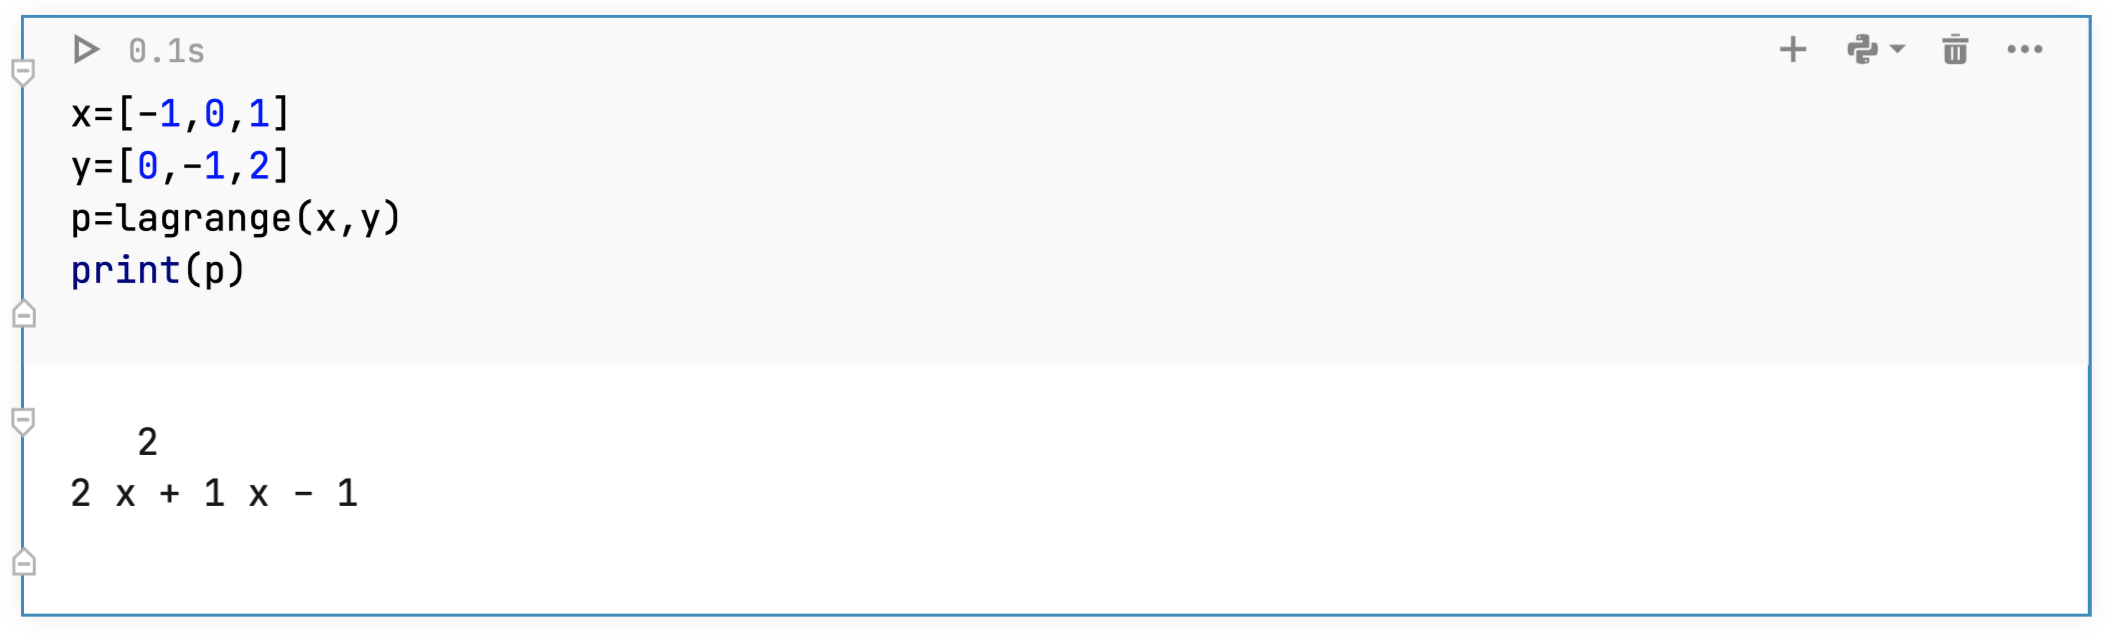
\includegraphics[width=5cm]{images/interpolationDeLagrange01.png}
\begin{tabular}{c}
\begin{tikzpicture}[domain=1.1:4.9,scale=0.6]
   \draw[->] (0.5,-0.4) -- (5.1,-0.4) node[above] {$\scriptstyle x$};
    \draw[->] (0.7,-0.5) -- (0.7,2.2) node[above] {$\scriptstyle y$};
   \path[fill=black]  (1.2,0.432) circle (.5mm) [fill=gray];
    \path[fill=black]  (2,1) circle (.5mm) [fill=gray];
    \path[fill=black]  (3,0) circle (.5mm) [fill=gray];
     \path[fill=black]  (4,2) circle (.5mm) [fill=gray];
      \path[fill=black]  (4.7,0.968) circle (.5mm) [fill=gray];
  %\draw[color=red,samples=200]    plot ( \x, {-0.625*\x^4+2.25*\x^3-0.875*\x^2-1.75*\x+2} )  ;
  \draw[color=red,samples=200]    plot ( \x, {-(\x-3)*(5*\x^3-43*\x^2+106*\x-72)/8} )  ;
  %\draw[color=red,samples=100,domain=0.05:3]    plot ( \x, {ln(1/sqrt(1+5/(exp(\x)-exp(-\x)))} )  ;
\end{tikzpicture}
\\
\begin{tikzpicture}[domain=0:5,scale=0.6]
   \draw[->] (-1,0) -- (5.1,0) node[above] {$\scriptstyle x$};
    \draw[->] (0,-0.5) -- (0,2) node[above] {$\scriptstyle y$};
   \path[fill=black]  (0.5,1.59) circle (.5mm) [fill=gray];
    \path[fill=black]  (1,1.95) circle (.5mm) [fill=gray];
    \path[fill=black]  (1.5,1.95) circle (.5mm) [fill=gray];
     \path[fill=black]  (2,1.59) circle (.5mm) [fill=gray];
      \path[fill=black]  (2.5,1) circle (.5mm) [fill=gray];
      \path[fill=black]  (3,0.415) circle (.5mm) [fill=gray];
    \path[fill=black]  (3.5,0.052) circle (.5mm) [fill=gray];
    \path[fill=black]  (4,0.052) circle (.5mm) [fill=gray];
    \path[fill=black]  (4.5,0.415) circle (.5mm) [fill=gray];
     \path[fill=black]  (5,1) circle (.5mm) [fill=gray];

  \draw[color=red,samples=200]    plot ( \x, {0.183*\x^3-1.394*\x^2+2.471*\x+0.702} )  ;
  %\draw[color=red,samples=200]    plot ( \x, {-(\x-3)*(5*\x^3-43*\x^2+106*\x-72)/8} )  ;
  %\draw[color=red,samples=100,domain=0.05:3]    plot ( \x, {ln(1/sqrt(1+5/(exp(\x)-exp(-\x)))} )  ;
\end{tikzpicture}
\end{tabular}



		\end{column}
		\begin{column}{.6\textwidth}
\begin{footnotesize}
	
\begin{itemize}
\item On cherche un polynôme $P$ qui interpole la fonction mesurée aux points $x_i$\\
$P(x_i) = f(x_i)$. 

\item On cherche P un polynôme le plus
proche des valeurs mesurées. L'approximation
au sens des moindre carré
consiste  à minimiser
\[\sum_i\left(P(x_i)-f(x_i)\right)^2\]
\end{itemize}

\end{footnotesize}
		\end{column}
	\end{columns}
 

  \end{frame}

  \begin{frame}
 
  \begin{block}{Applications}
   \begin{itemize}
  \item On cherche à calculer une intégrale dont on ne connaît pas explicitement sa valeur. Par exemple, on approche cette comme suit
\[f(x)\simeq p(x) \mbox{ et } \int f(x) dx \simeq\int P(x) dx \]
ce qui conduit à l'intégration numérique.
 \item $f$ solution d'une e.d.o
 \item $f$ solution d'une équation non linéaire de la forme $f = G(f)$
 \item Soit $f$ une fonction inconnue solution d'un problème aux limites (équation de la chaleur par exemple), on cherche à approcher au mieux les valeurs de $f$ en certains points du
domaine.
  \end{itemize}
  \end{block}
  
  
  \end{frame}

  \begin{frame}
	\frametitle{Interpolation de Lagrange}
	\begin{block}{Théorème}
	
		Soit $f : [a, b] \to \mathbb{R}$ une fonction continue et $x_0<x_1<\cdots <x_n$, 
$n + 1$ points distincts de $[a, b]$. Il existe un unique $P \in \mathbb{R}_n[X]$ tel que $P(x_i) = f(x_i)$ pour $i = 0, 1, ..., n$.
De plus, $P$ est donné par :
\[\myredbox{P(x)=\sum_{i=0}^nf(x_i) L_i(x)}\]
où les polynômes $L_i$ sont définis par : $L_i(x)=\prod_{j=0,j\neq i}^n\frac{x-x_j}{x_i-x_j}$

	
	
	\end{block}
	Démonstration
	\begin{itemize}
  	\item Unicité. Soient $P, Q \in \mathbb{R}_n[X]$ tels que $P(x_i) = Q(x_i) = f_i$ pour
  	 $i = 0, ...n$, alors $P - Q \in \mathbb{R}_n[X]$ et il s'annule en $n + 1$ points distincts alors $P - Q \equiv 0$.
	\item Existence. On pose $P(x)=\sum_{i=0}^nf(x_i) L_i(x)$
  \end{itemize}	 
	
\end{frame}


\begin{frame}
%\lipsum[2]

	\begin{itemize}
  	\item \fbox{$n=1$} deux points de discrétisation $x_0=0$ et $x_1=1$.
  	
  	\begin{center}
  	\begin{tabular}{cc}
 \begin{tikzpicture}[scale=2]
\draw  [very thin, gray] [->]  (-0.2,0) -- (1.2,0); 
\draw  [very thin, gray] [->] (0,-0.2) -- (0,1.2);
\draw  [dashed] (0,0) -- (0,1);
\node [blue] at (0,0) {$\bullet$};
\node [blue] at (1,0) {$\bullet$};
\node at (0.5,-0.5) {$\scriptstyle  L_0(x)=1-x$};
\draw [orange,domain=0:1] plot(\x,1-\x);

\end{tikzpicture} 
  &
   \begin{tikzpicture}[scale=2]
\draw  [very thin, gray] [->]  (-0.2,0) -- (1.2,0); 
\draw  [very thin, gray] [->] (0,-0.2) -- (0,1.2);
\draw  [dashed] (1,0) -- (1,1);
\node [blue] at (0,0) {$\bullet$};
\node [blue] at (1,0) {$\bullet$};
\node at (0.5,-0.5) {$\scriptstyle L_1(x)=x$};
\draw [orange,domain=0:1] plot(\x,\x);

\end{tikzpicture} 
\end{tabular}
  	\end{center}
  	
	\item \fbox{$n=2$} trois points de discrétisation $x_0=0$ , $x_1=\frac 12$ et $x_2=1$.
  	\begin{center}
  	\begin{tabular}{ccc}
 \begin{tikzpicture}[scale=2]
\draw  [very thin, gray] [->]  (-0.2,0) -- (1.2,0); 
\draw  [very thin, gray] [->] (0,-0.2) -- (0,1.2);
\draw  [dashed] (0,0) -- (0,1);
\node [blue] at (0,0) {$\bullet$};
\node [blue] at (0.5,0) {$\bullet$};
\node [blue] at (1,0) {$\bullet$};
\node at (0.5,-0.5) {$\scriptstyle L_0(x)=(2x-1)(x-1)$};
\draw [orange,domain=0:1] plot(\x,{(2*\x-1)*(\x-1)});

\end{tikzpicture} 
  &
  \begin{tikzpicture}[scale=2]
\draw  [very thin, gray] [->]  (-0.2,0) -- (1.2,0); 
\draw  [very thin, gray] [->] (0,-0.2) -- (0,1.2);
\node [blue] at (0,0) {$\bullet$};
\node [blue] at (0.5,0) {$\bullet$};
\node [blue] at (1,0) {$\bullet$};
\node at (0.5,-0.5) {$\scriptstyle L_1(x)=4x(1-x)$};
\draw [orange,domain=0:1] plot(\x,{4*\x*(1-\x)});

\end{tikzpicture} 
  &
  \begin{tikzpicture}[scale=2]
\draw  [very thin, gray] [->]  (-0.2,0) -- (1.2,0); 
\draw  [very thin, gray] [->] (0,-0.2) -- (0,1.2);
\draw  [dashed] (1,0) -- (1,1);
\node [blue] at (0,0) {$\bullet$};
\node [blue] at (0.5,0) {$\bullet$};
\node [blue] at (1,0) {$\bullet$};
\node at (0.5,-0.5) {$\scriptstyle L_2(x)=x(2x-1)$};
\draw [orange,domain=0:1] plot(\x,{\x*(2*\x-1)});

\end{tikzpicture} 
\end{tabular}
  	\end{center}
	
  \end{itemize}	
 \end{frame}  

\begin{frame}
 \frametitle{Exemple}

On cherche le polynôme d'interpolation de LAGRANGE qui en $x_1$ vaut $y_1$, en $x_2$ vaut $y_2$. On a
\begin{footnotesize}


\[P(x)=y_1\frac{x-x_2}{x_1-x_2}+y_2\frac{x-x_1}{x_2-x_1}\]

\[P(x)=-y_1\frac{x-x_2}{h}+y_2\frac{x-x_1}{h}\]
\[P(x)=\frac{y_2-y_1}{x_2-x_1}(x-x_1)+y_1\]

\end{footnotesize}

\begin{center}
 \begin{tikzpicture}[scale=0.7]
\draw  [very thin, gray] [->]  (-0.2,0) -- (4,0) node[right] {$\scriptstyle x$};
\draw  [very thin, gray] [->] (0,-0.3) -- (0,2.2) node[above] {$\scriptstyle y$};
\node [blue] at (1,1) {$\bullet$};
\draw  [dotted] (1,0) -- ++(0,1.2) node[above] {$\scriptstyle y_1$};
\node [blue] at (3,2) {$\bullet$};
\draw  [dotted] (3,0) -- ++(0,2.2) node[above] {$\scriptstyle y_2$};
%\node at (0.5,-0.5) {$\scriptstyle L_0(x)=(2x-1)(x-1)$};
\draw [orange,domain=-0.5:4] plot(\x,{(\x+1)/2});

\end{tikzpicture} 
\end{center}
\end{frame}


 \begin{frame}
 \frametitle{Exemple}

On cherche le polynôme d'interpolation de LAGRANGE qui en $-1$ vaut $0$, en $0$ vaut $-1$ et en $1$ vaut $2$. On a
\begin{footnotesize}


\[P(x)=y_0\frac{(x-x_1)(x-x_2)}{(x_0-x_1)(x_0-x_2)}+y_1\frac{(x-x_0)(x-x_2)}{(x_1-x_0)(x_1-x_2)}+y_2\frac{(x-x_0)(x-x_1)}{(x_2-x_0)(x_2-x_1)}\]

\[P(x)=0\times\frac{x(x-1)}{2}+(-1)\times\frac{(x+1)(x-1)}{-1}+2\times\frac{(x+1)x}{2}=2x^2+x-1\]

\end{footnotesize}

\begin{center}
 \begin{tikzpicture}[scale=0.7]
\draw  [very thin, gray] [->]  (-1.2,0) -- (1.2,0); 
\draw  [very thin, gray] [->] (0,-1.3) -- (0,3.2);
\node [blue] at (-1,0) {$\bullet$};
\node [blue] at (0,-1) {$\bullet$};
\node [blue] at (1,2) {$\bullet$};
%\node at (0.5,-0.5) {$\scriptstyle L_0(x)=(2x-1)(x-1)$};
\draw [orange,domain=-1.5:1.2] plot(\x,{(2*\x-1)*(\x+1)});

\end{tikzpicture} 
\end{center}
\end{frame}

\begin{frame}
 \frametitle{Code python}
 \begin{center}

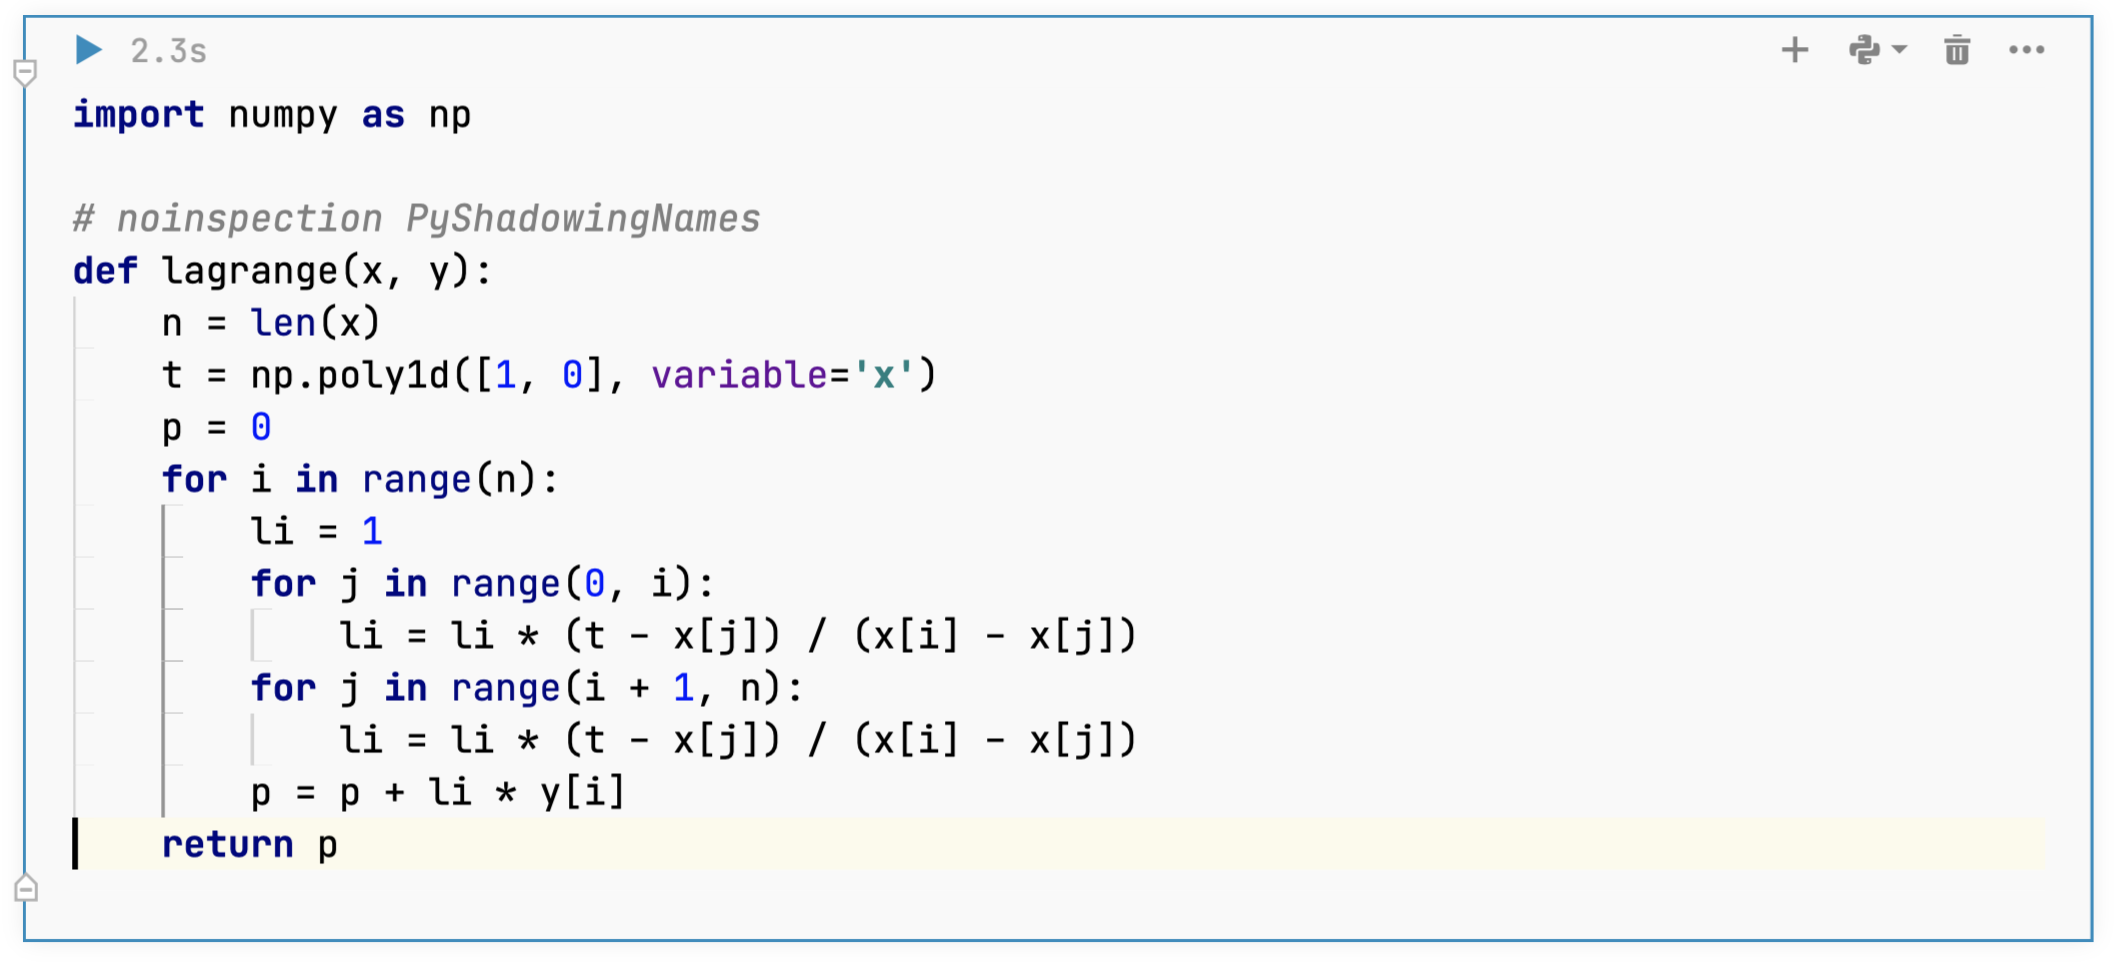
\includegraphics[width=10cm]{images/interpolationDeLagrange00.png}
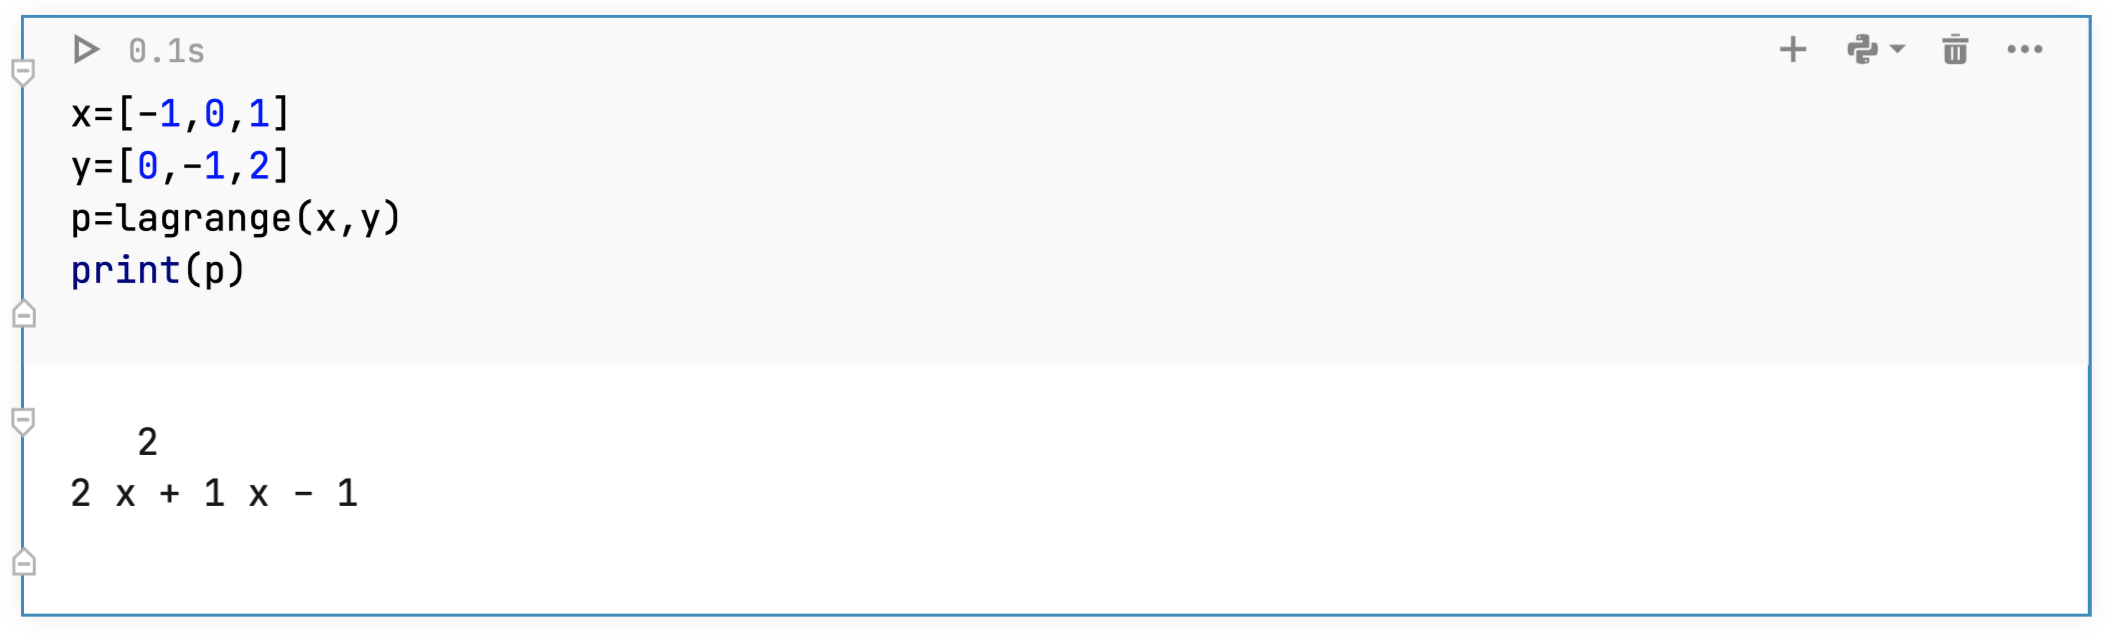
\includegraphics[width=10cm]{images/interpolationDeLagrange01.png}
\end{center}
\end{frame}

 \begin{frame}
 \frametitle{Exemple}
 Interpolation polynomiale de $\sin$ en six  points:

\begin{center}
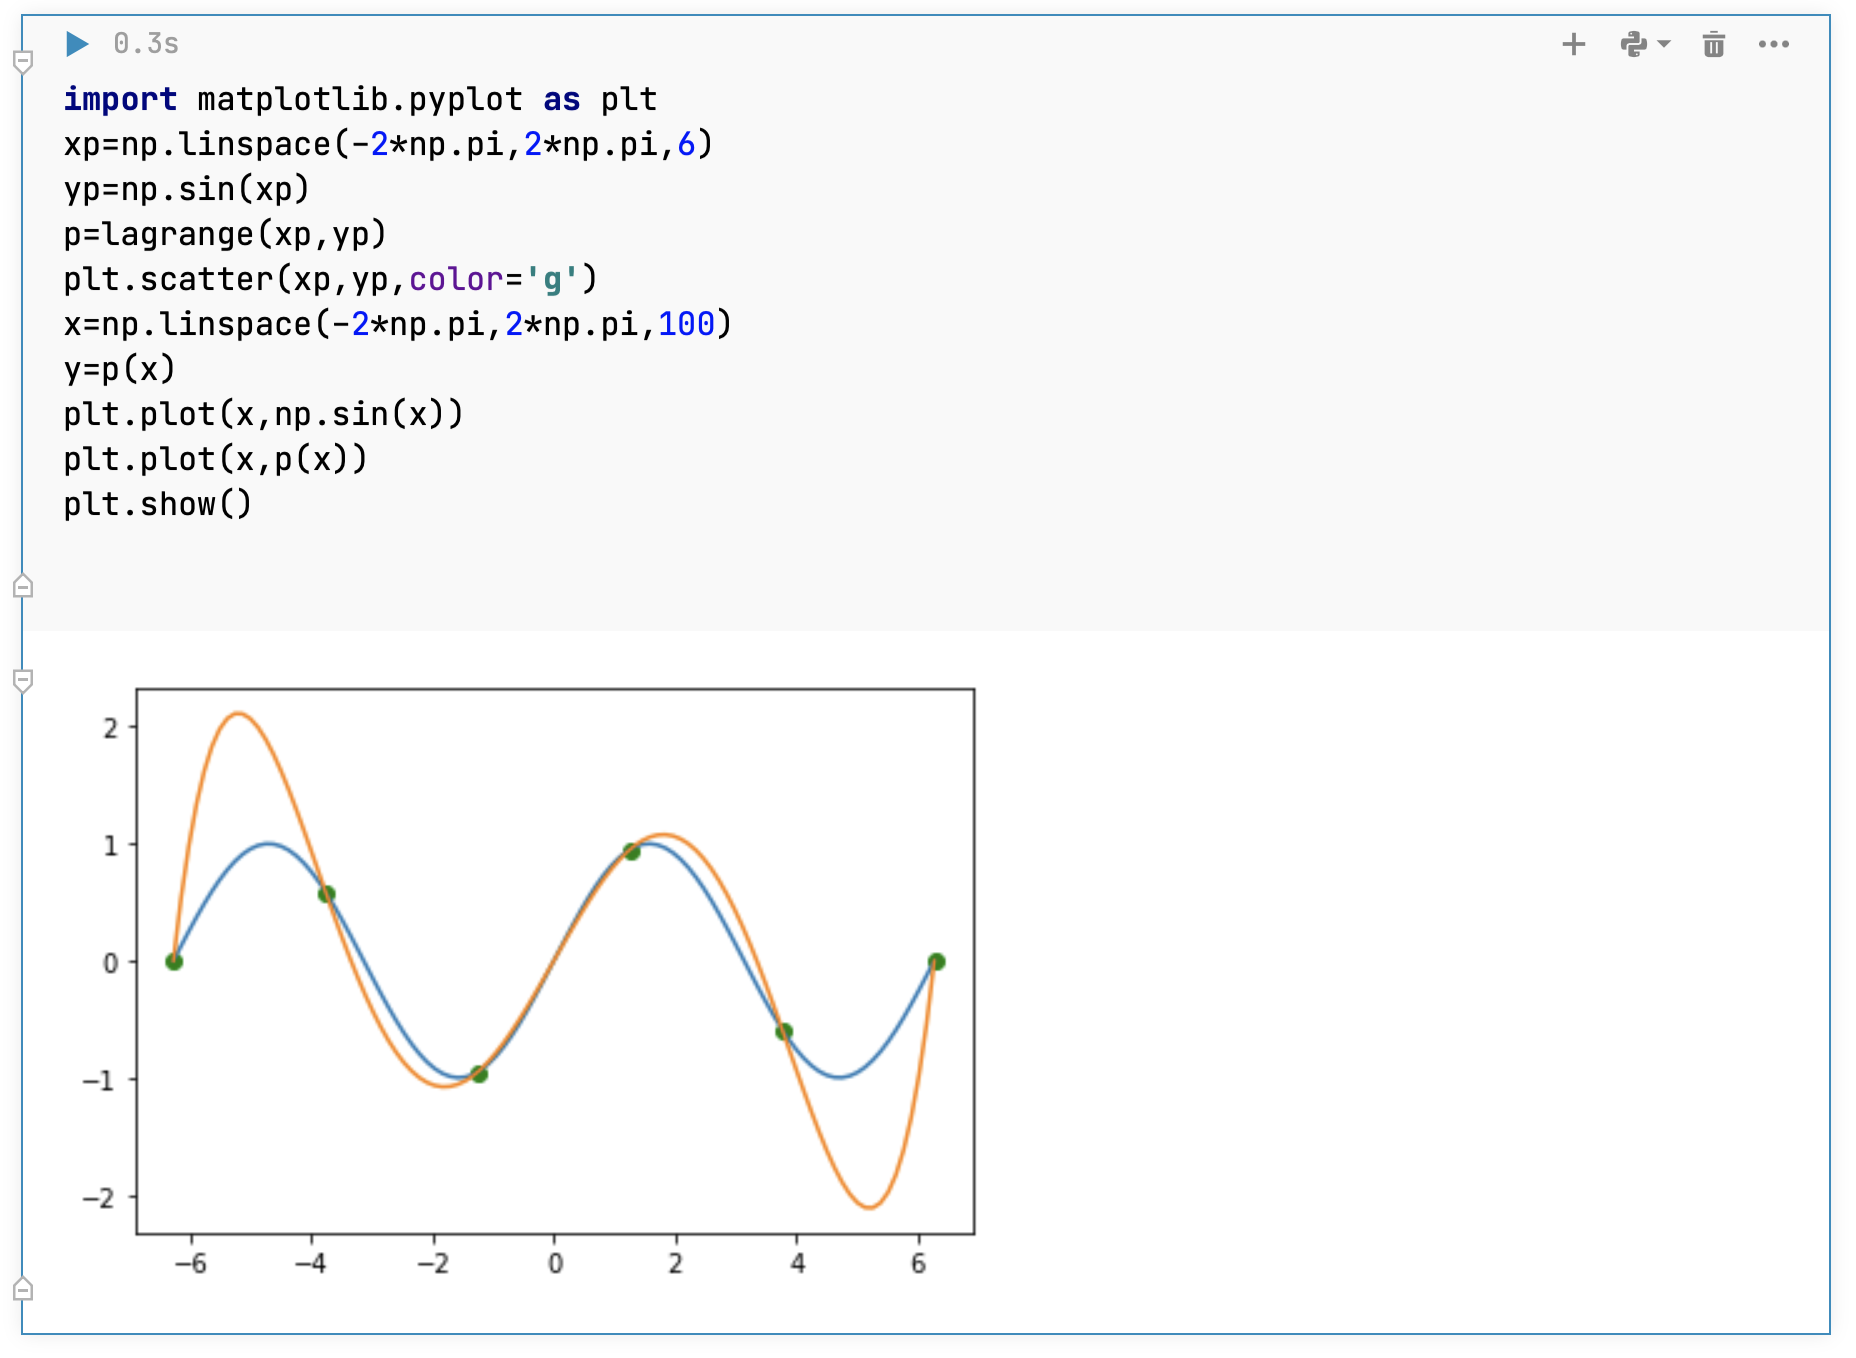
\includegraphics[width=10cm]{images/interpolationDeLagrange02.png}
\end{center}

\end{frame}

 \begin{frame}
 \frametitle{Exemple}
 Interpolation polynomiale de $\sin$ en dix  points:

\begin{center}
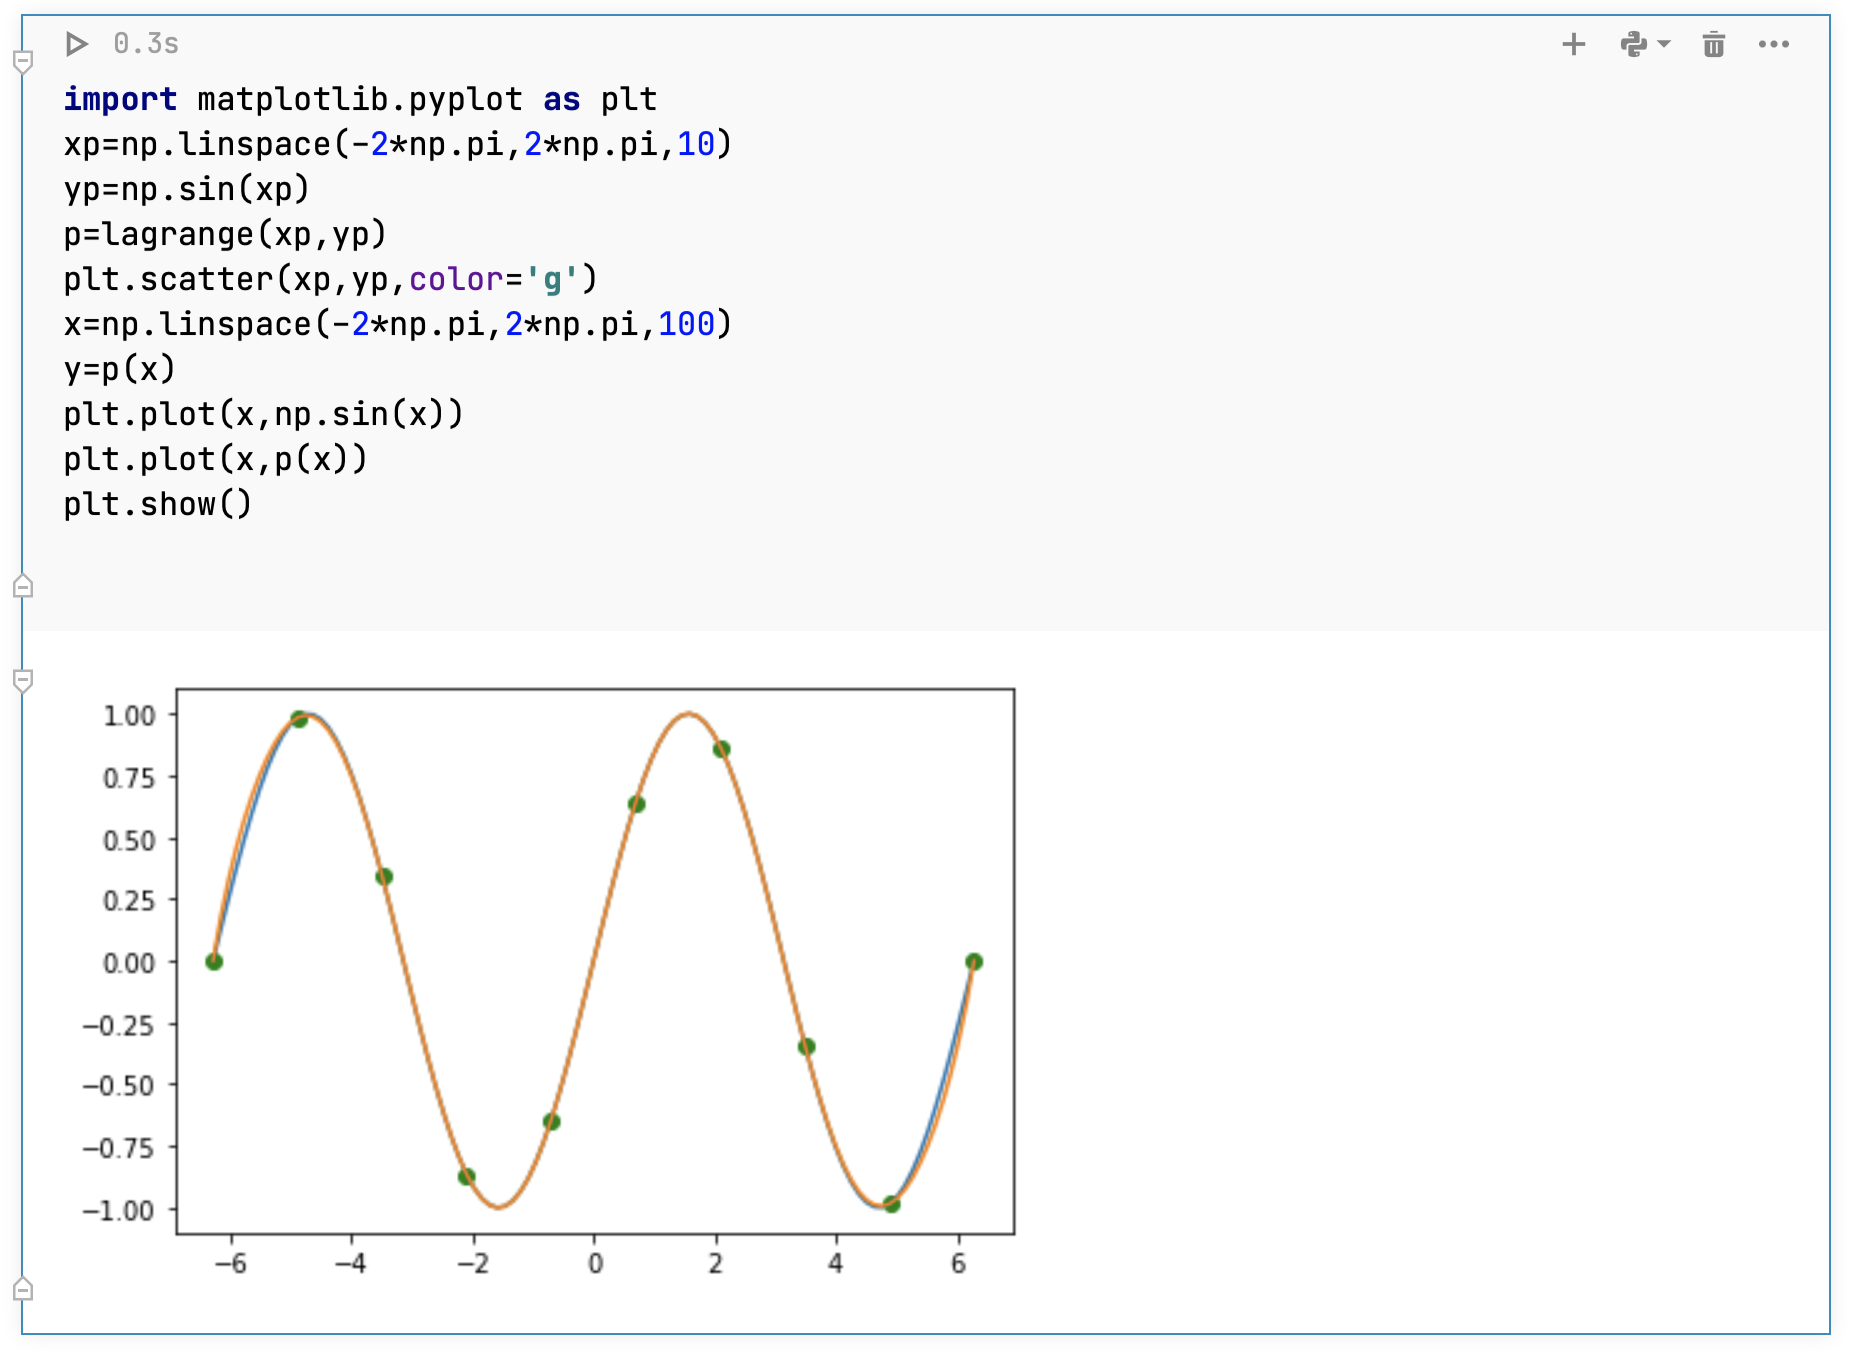
\includegraphics[width=10cm]{images/interpolationDeLagrange03.png}
\end{center}

\end{frame}

 \begin{frame}
 \frametitle{Exemple}
 Interpolation polynomiale de $x\mapsto \frac 1{x^2+1}$ en 8  points:
\begin{center}
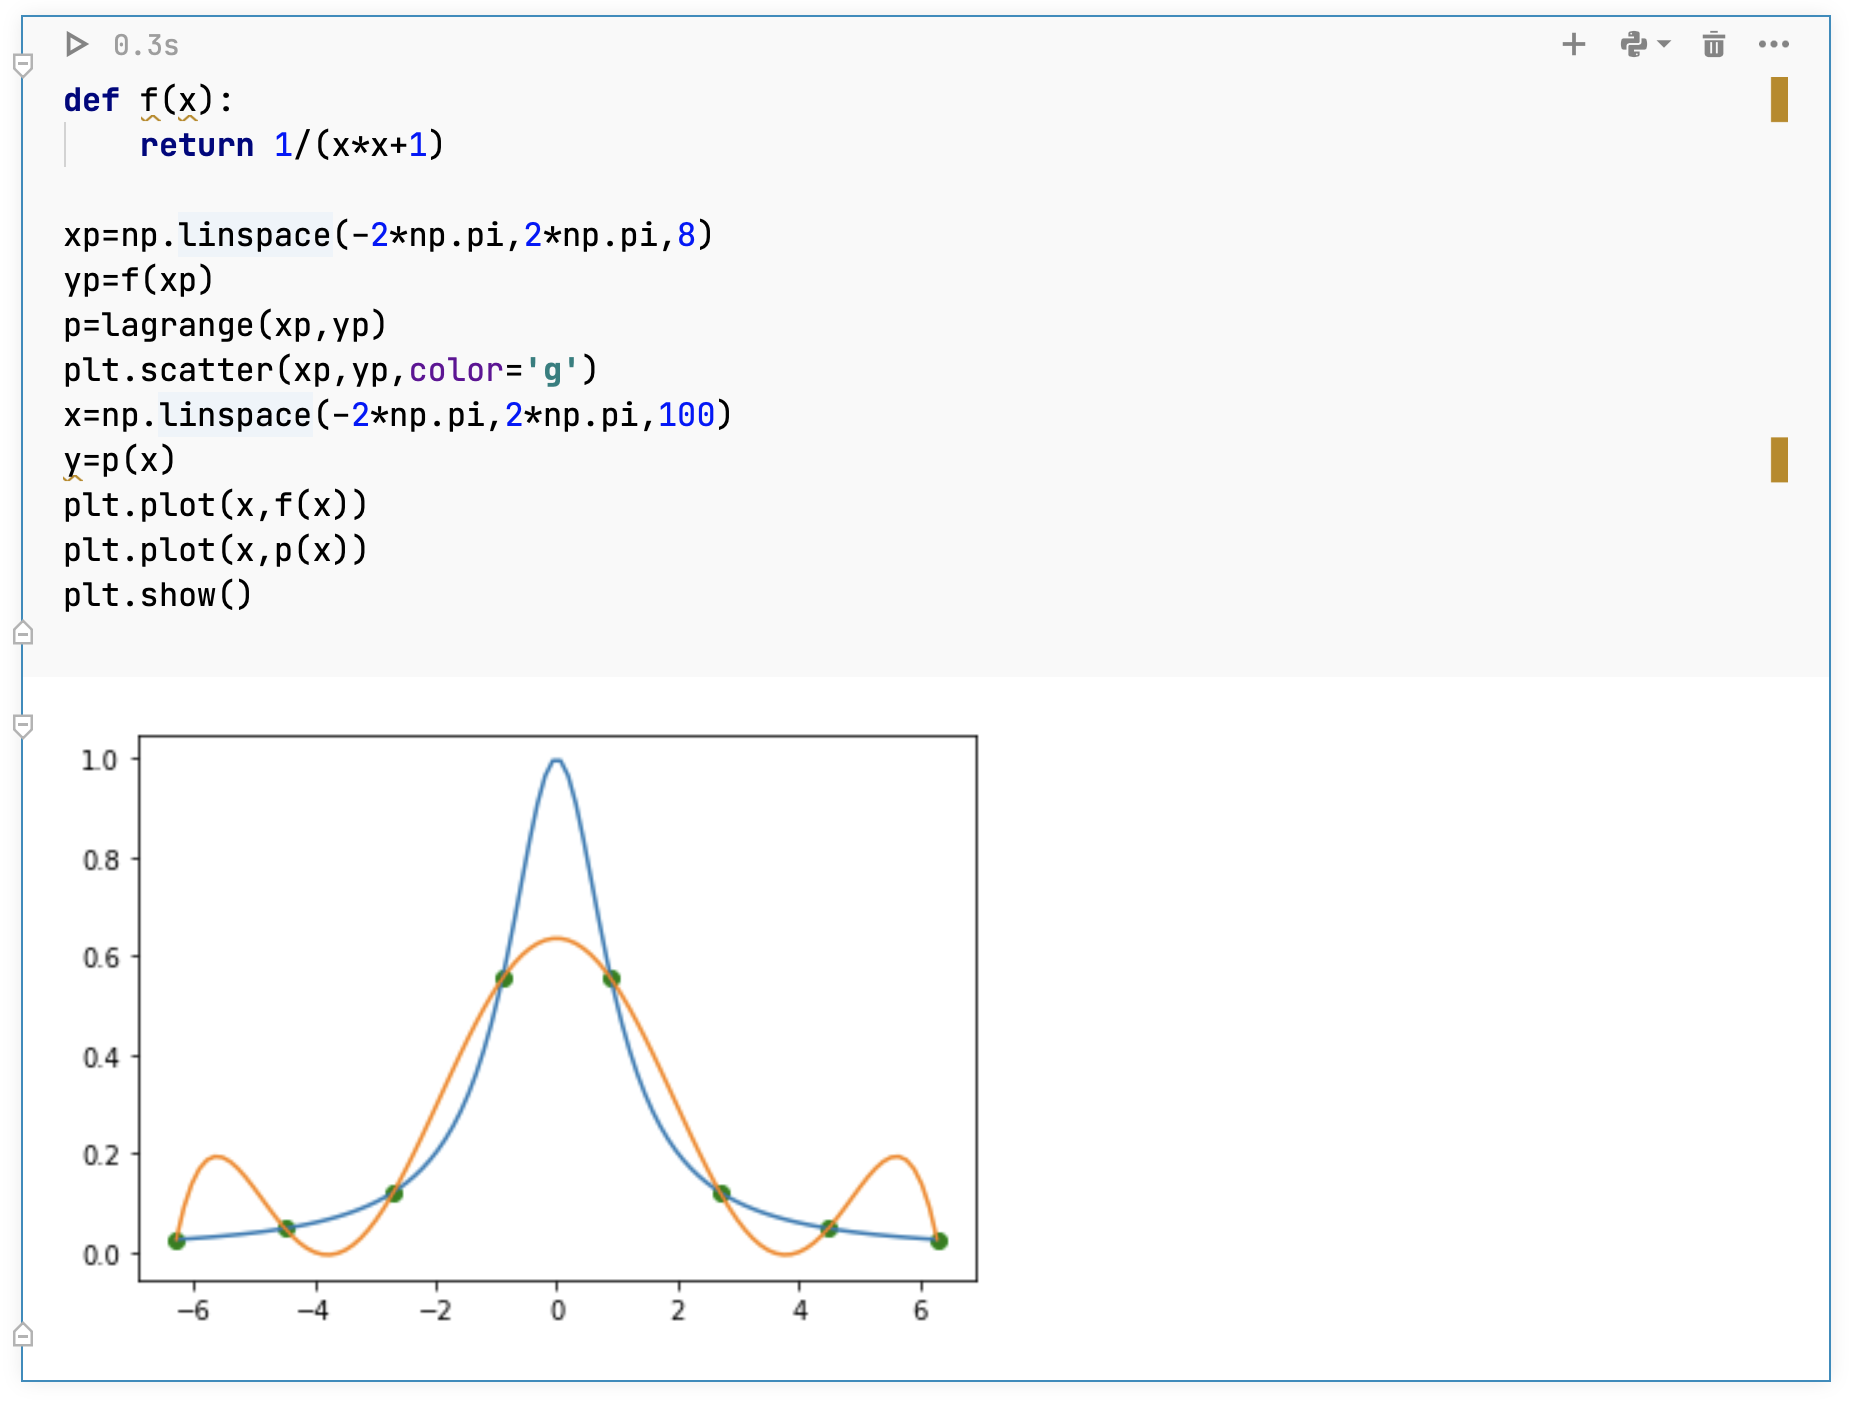
\includegraphics[width=10cm]{images/interpolationDeLagrange04.png}
\end{center}

\end{frame}

 \begin{frame}
 \frametitle{Exemple}
 Interpolation polynomiale de $x\mapsto \frac 1{x^2+1}$ en  11 points:
\begin{center}
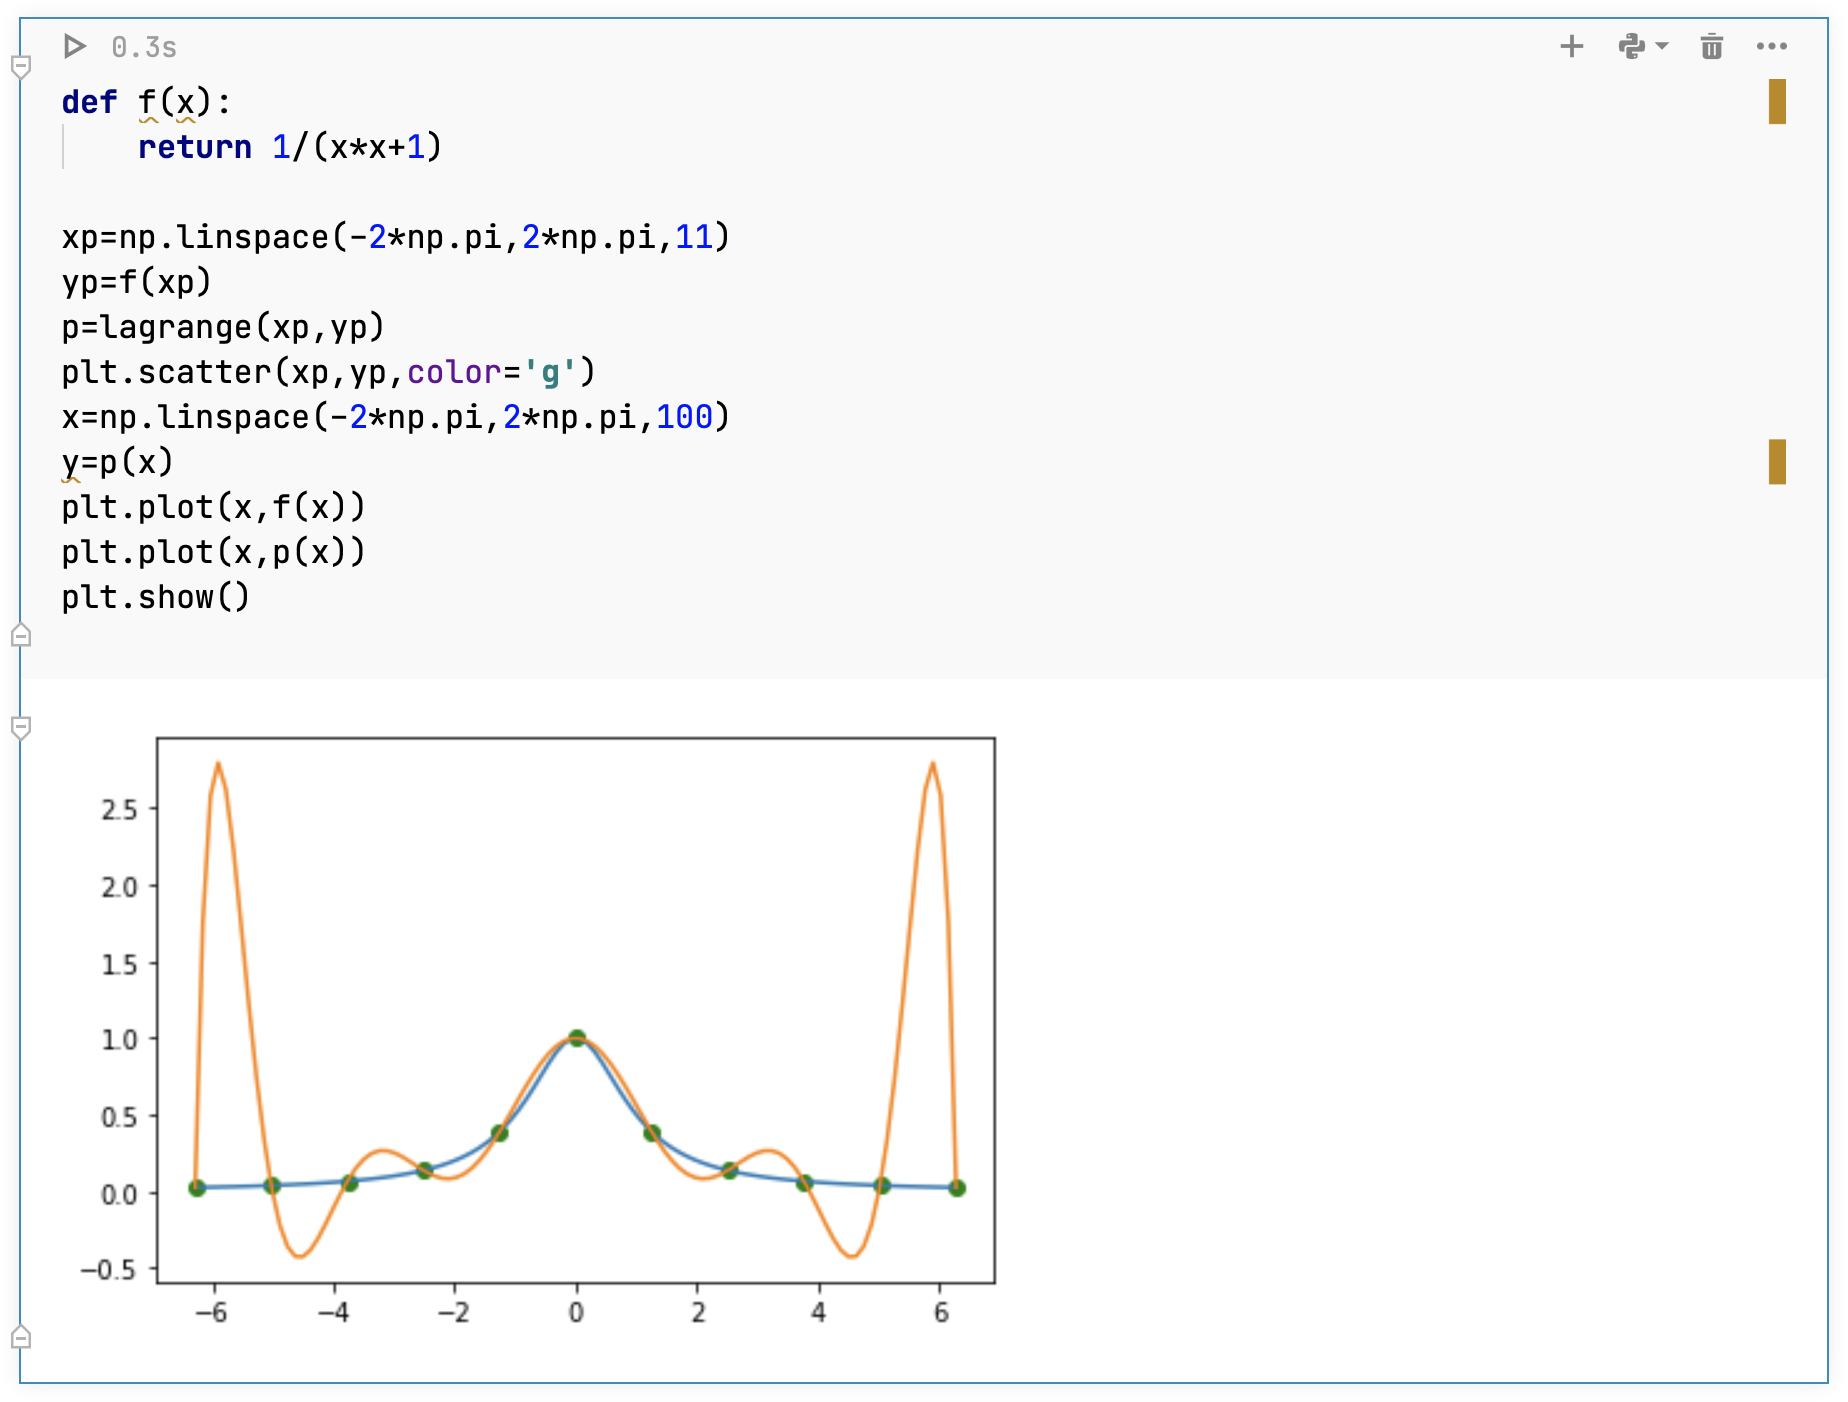
\includegraphics[width=10cm]{images/interpolationDeLagrange05.png}
\end{center}

\end{frame}


\begin{frame}
 \frametitle{Exemple}

Problème d'échantillonnage: $T_e<T/2$?.

\begin{center}
 \begin{tikzpicture}[xscale=0.7]
\draw  [gray] [->]  (-6.5,0) -- (6.5,0); 
\draw  [gray] [->] (0,-1.3) -- (0,1.2);
 \path[fill=black]  (-6.28,0) circle (.8mm) [fill=gray];
 \path[fill=black]  (6.28,0) circle (.8mm) [fill=gray];
  \path[fill=black]  (-5.14,-0.54) circle (.8mm) [fill=gray];
  \path[fill=black]  (5.14,0.54) circle (.8mm) [fill=gray];
   \path[fill=black]  (-3.99,-0.909) circle (.8mm) [fill=gray];
    \path[fill=black]  (3.99,0.909) circle (.8mm) [fill=gray];
    \path[fill=black]  (-2.85,-0.989) circle (.8mm) [fill=gray];
     \path[fill=black]  (2.85,0.989) circle (.8mm) [fill=gray];
     \path[fill=black]  (-1.713,-0.755) circle (.8mm) [fill=gray];
     \path[fill=black]  (1.713,0.755) circle (.8mm) [fill=gray];
      \path[fill=black]  (-0.571,-0.281) circle (.8mm) [fill=gray];
       \path[fill=black]  (0.571,0.281) circle (.8mm) [fill=gray];
     
%\node at (0.5,-0.5) {$\scriptstyle L_0(x)=(2x-1)(x-1)$};
\draw [orange,samples=200,domain=-6.5:6.5] plot(\x,{sin(5*\x r)});
\draw [blue,samples=200,domain=-6.5:6.5] plot(\x,{sin(0.5*\x r)});

\end{tikzpicture} 
\end{center}
\end{frame}



\begin{frame}
\begin{block}{Théorème(Erreur d'interpolation de Lagrange)}
Soit $f \in C^{n+1}([a, b])$ et $a \leq x_0 < x_1 < x_2 < ... < x_n \leq b$. Soit $P$ le polynôme de Lagrange défini par $P(x_i) = f(x_i)$ pour $i = 0, 1, ..., n$.
Alors
\[\myredbox{f(x) - P(x) =\frac{L(x)}{(n + 1)!}f^{(n+1)}(\xi)}\]
où $L(x)=\prod_{i=0}^n\left(x-x_i\right)$ et $a < \xi < b$.
\end{block}
L'erreur d'interpolation dépend alors de $\Lambda_n=\max_{x\in[a,b]}\left|L(x)\right|$ appelée constante de Lebesgue. Dans l'exemple précédent:
  \[x_i = a + i\frac{b-a}{n}, i=0,1,\cdots , n\]

La constante de Lebesgue sur l'intervalle $[-1, 1]$ est alors:

\[\Lambda_n \sim \frac{2^{n+1}}{\mbox{e}\, n\ln(n)}\]


\end{frame}

 \begin{frame}
  \frametitle{Polynôme de Tchebychev}
\[T_n(x) = \cos(n \arccos(x)),\quad x \in [-1, 1],\quad n\geq0\]
ou bien  \[T_0 =  1 , T_1(x) = x \mbox{ et } T_{n+1}(x) = 2 x T_n(x)-T_{n-1}(x)\] 
la constante de Lebesgue est beaucoup plus petite dans le cas des racines de polynôme de
Chebyshev:

\[\myredbox{x_i = \frac{a+b}2 + \cos\left(\frac{(2i + 1)\pi}
{2n}\right)\times \frac{b-a}{2},\quad i=0,1,\cdots , n-1}\]
La constante de Lebesgue sur l'intervalle $[-1, 1]$ est évaluée par l'équivalence:
\[\Lambda_n \sim \frac{2}{\pi}\, \ln(n)\]


\end{frame}

 \begin{frame}
 \frametitle{Exemple}
 Interpolation polynomiale de $x\mapsto \frac 1{x^2+1}$ en 11 points de Tchebychev:
\begin{center}
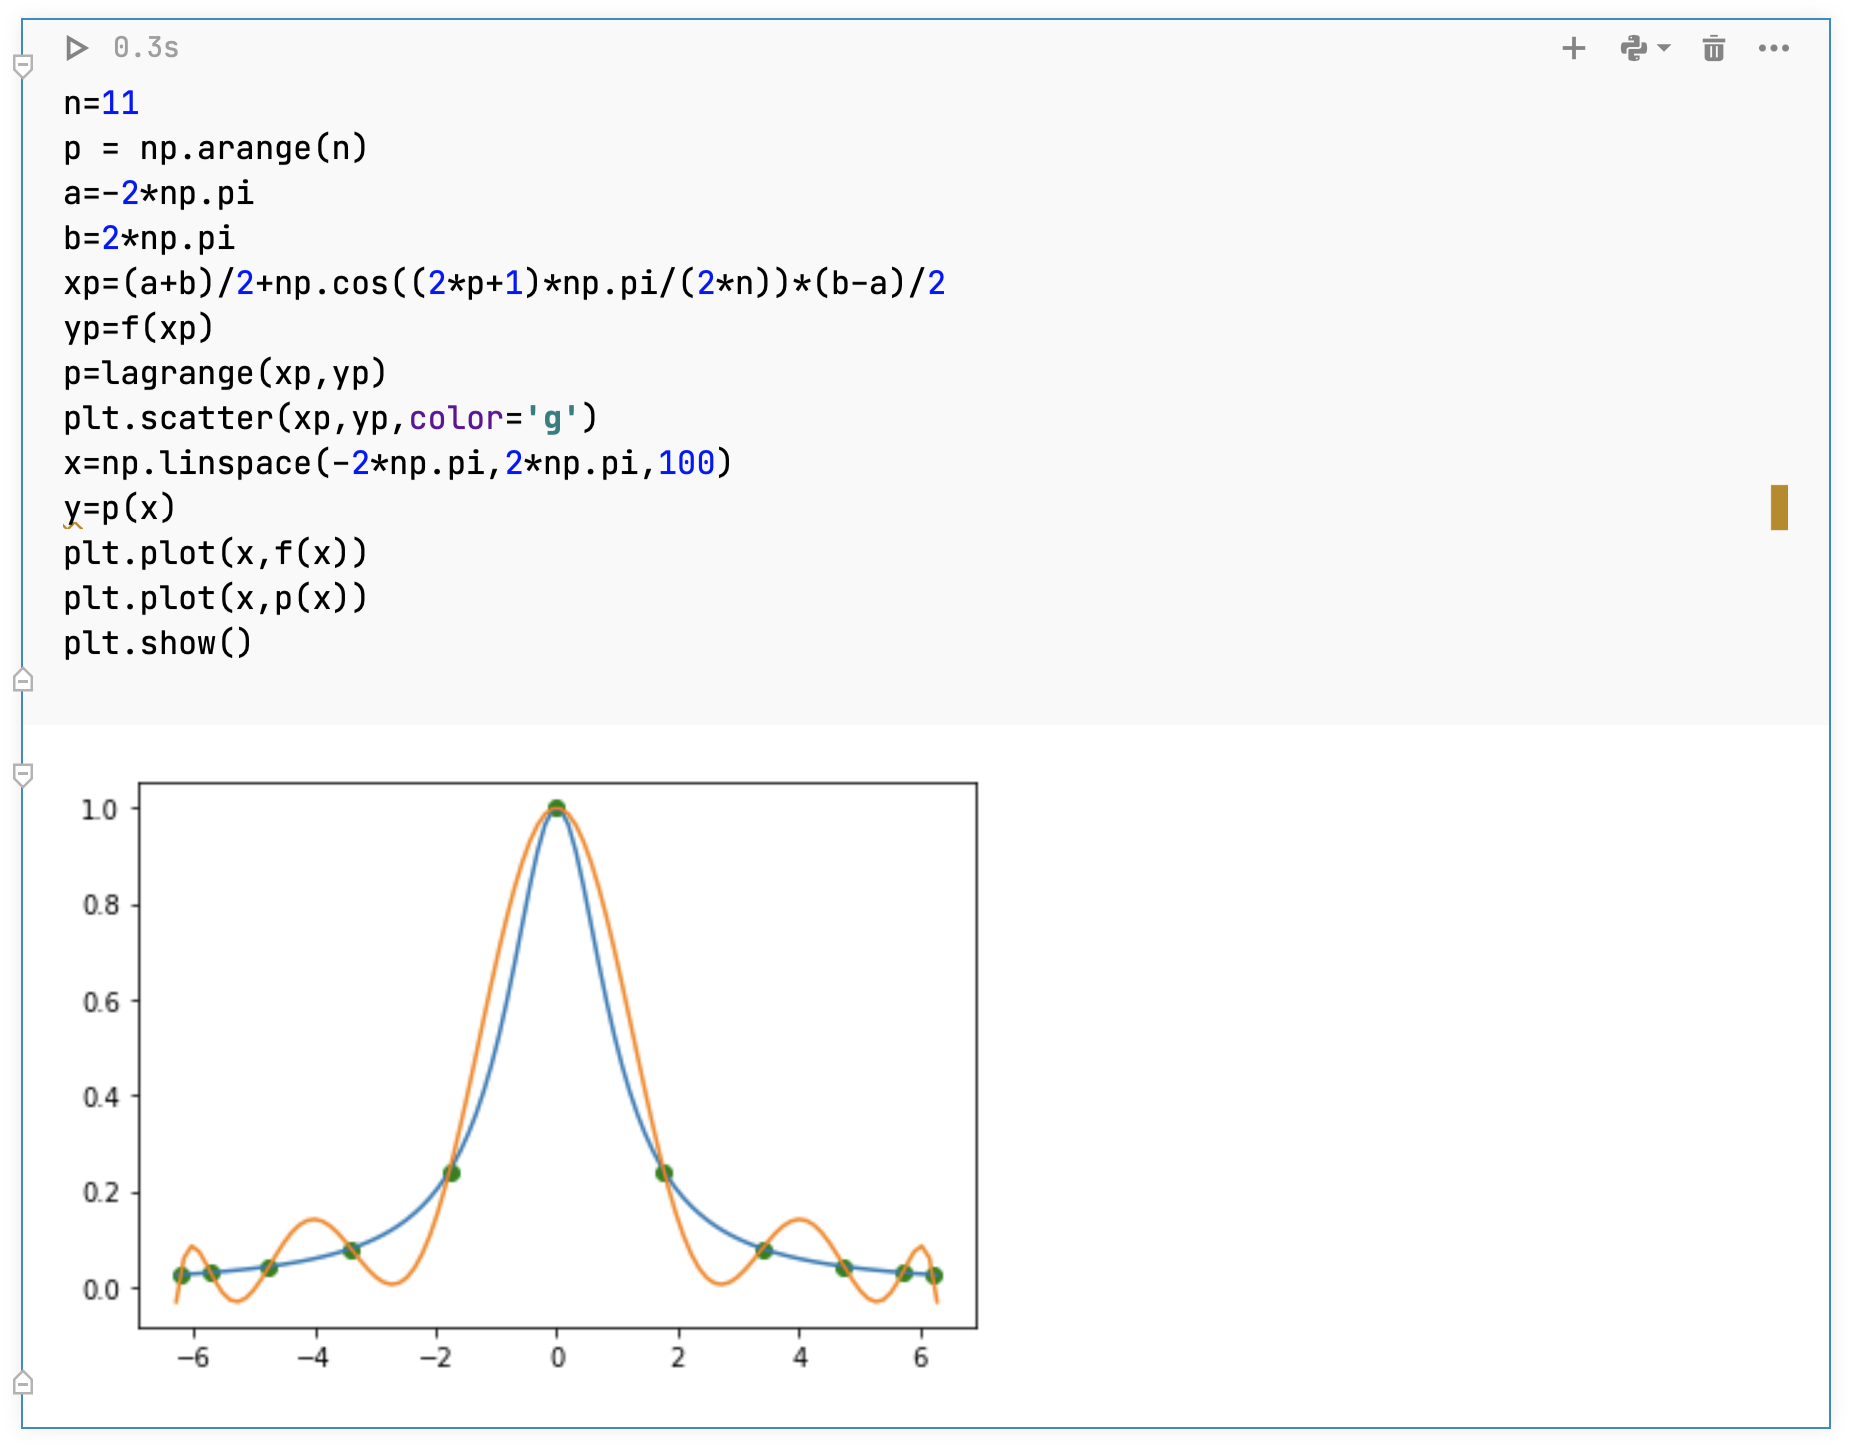
\includegraphics[width=10cm]{images/interpolationDeLagrange06.png}
\end{center}
\end{frame}

 \begin{frame}
 \frametitle{Exemple}
 Interpolation polynomiale de $x\mapsto \frac 1{x^2+1}$ en 19 points de Tchebychev:
\begin{center}
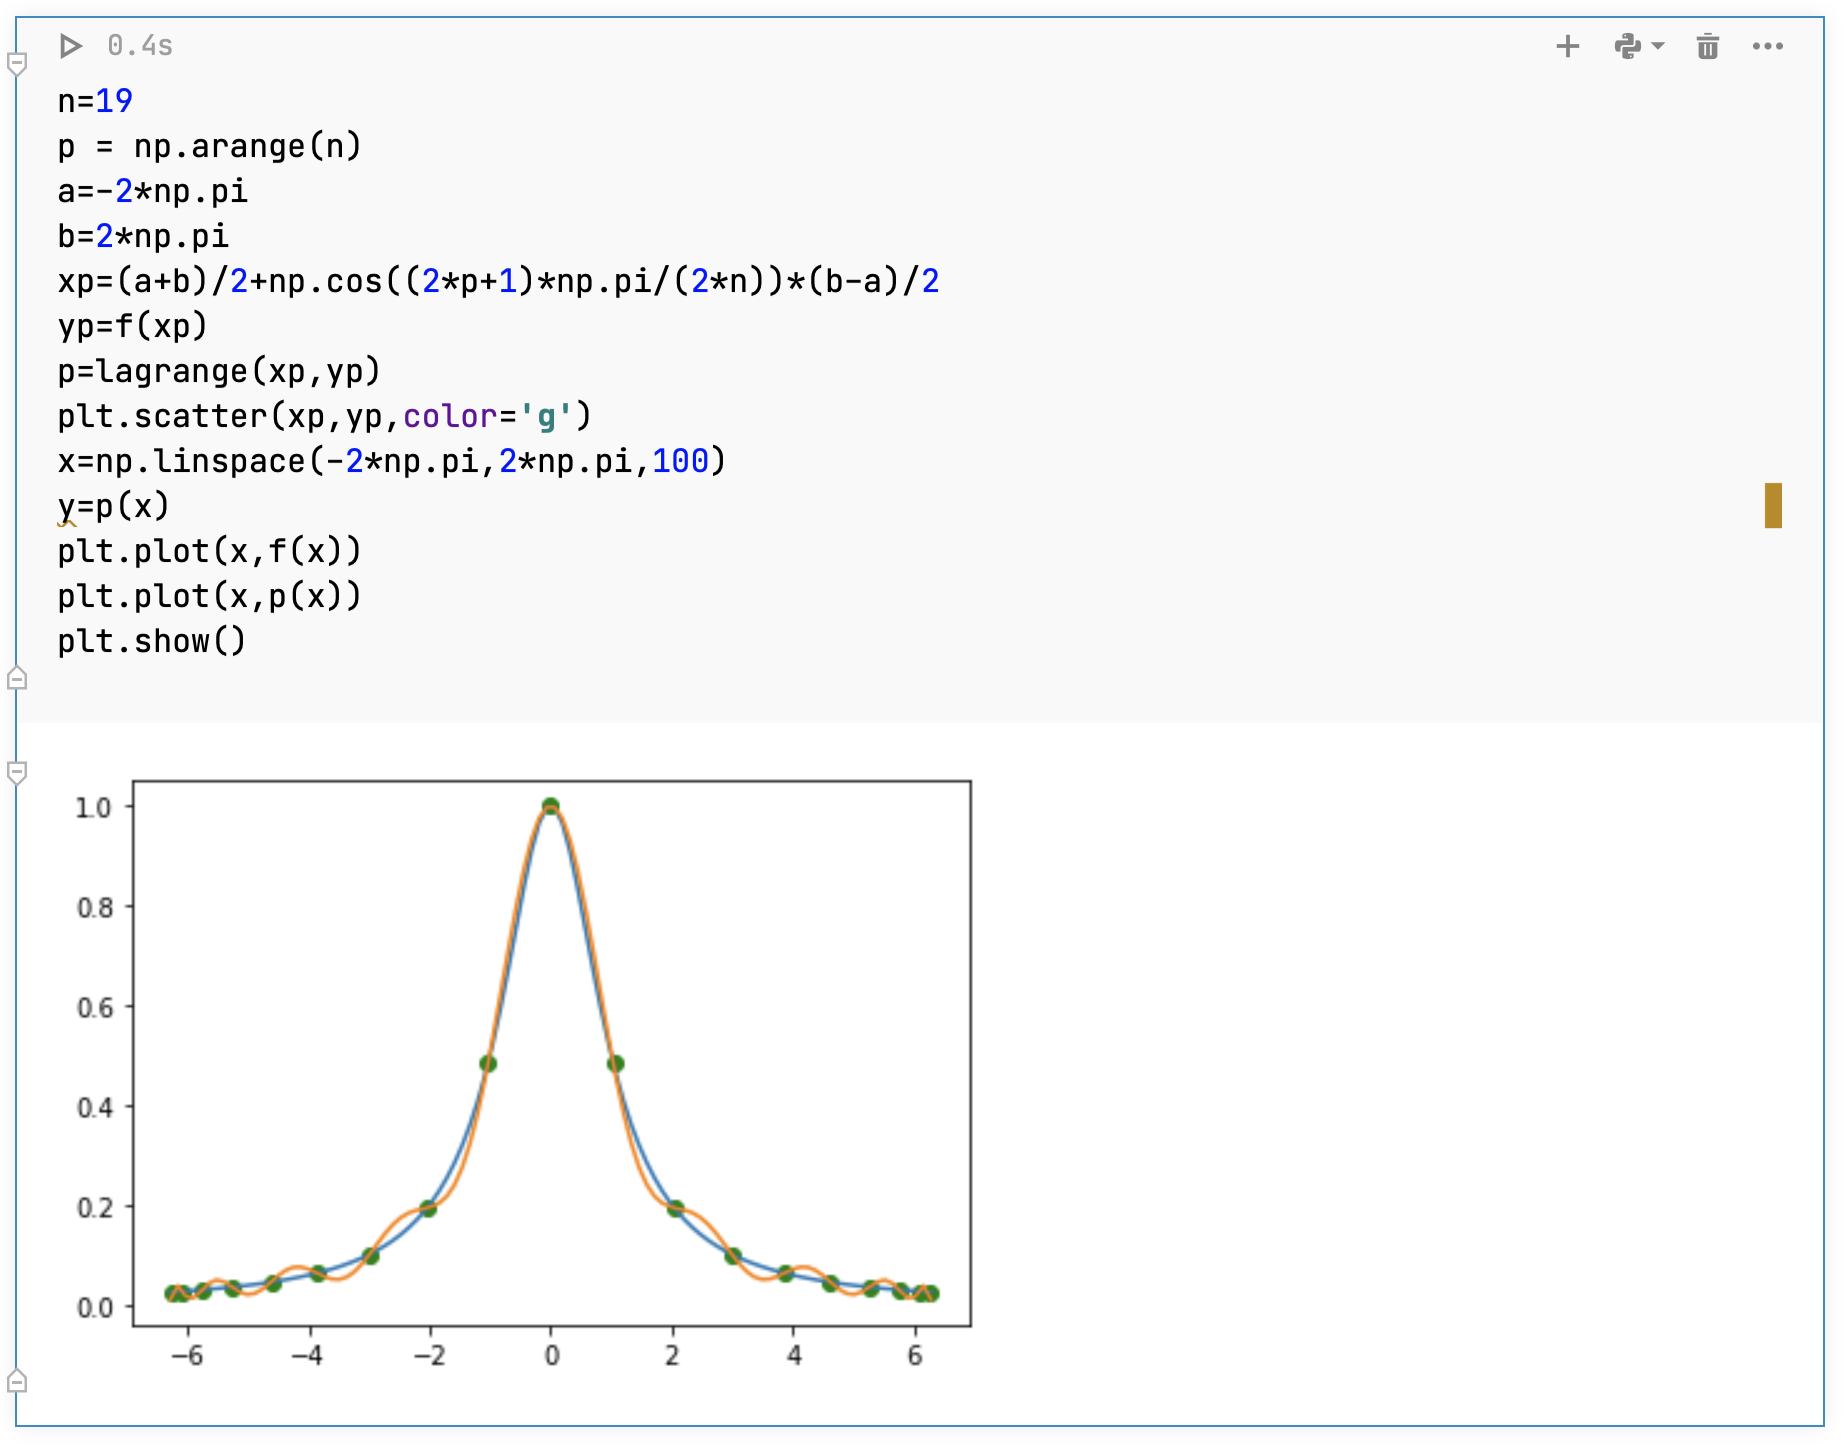
\includegraphics[width=10cm]{images/interpolationDeLagrange07.png}
\end{center}
\end{frame}

\begin{frame}
 \frametitle{Méthode de différences divisées}
 La formule de Lagrange n'a qu'un intérêt théorique. En pratique  on utilise plutôt une méthode de Newton dite de différences divisées:
 
 
\begin{itemize}
  \item $\Delta_1([x_1],[y_1])=y_1$
  \item si $n>1$ on pose $\Delta([x_1,\cdots,x_n],[y_1,\cdots,y_n])=$
 {\small  \[\frac{\Delta([x_2,\cdots,x_n],[y_2,\cdots,y_n])-\Delta([x_1,\cdots,x_{n-1}],[y_1,\cdots,y_{n-1}])}{x_n-x_1}\]}
 \end{itemize}
 

Si on pose $\Delta_k=\Delta([x_1,\cdots,x_k],[y_1,\cdots,y_k])$, le polynôme d'interpolation s'écrit:
\[ P=\sum_{k=1}^n\Delta_k\prod_{j=1}^{k-1}(x-x_j)\]
\end{frame}

\begin{frame}
Pour expliciter le processus récursif, les différences divisées peuvent être calculées en les disposant de la manière suivante dans un tableau :
\begin{footnotesize}
\[\begin{array}{cc|cccc}\hline
x_i&y_i&\Delta[x_{i-1},x_i]&\Delta[x_{i-2},x_{i-1},x_i]&\Delta[x_{i-3},x_{i-2},x_{i-1},x_i]&\Delta[x_{i-4},x_{i-3},x_{i-2},x_{i-1},x_i]\\ \hline\hline
x_0&\boxed{y_0}&&&& \\
x_1&y_1&\boxed{\Delta[x_0,x_1]}&&& \\
x_2&y_2&\Delta[x_1,x_2]&\boxed{\Delta[x_0,x_1,x_2]}&& \\
x_3&y_3&\Delta[x_2,x_3]&\Delta[x_1,x_2,x_3]&\boxed{\Delta[x_0,x_1,x_2,x_3]}& \\
x_4&y_4&\Delta[x_3,x_4]&\Delta[x_2,x_3,x_4]&\Delta[x_1,x_2,x_3,x_4]&\boxed{\Delta[x_0,x_1,x_2,x_3,x_4]} \\
\vdots &\vdots &\vdots &\vdots &\vdots &\vdots 
\end{array}
\]
\end{footnotesize}
\end{frame}



\begin{frame}
On reprend le polynôme d'interpolation de LAGRANGE qui en $-1$ vaut $1$, en $0$ vaut $-1$ et en $1$ vaut $2$. On a

\[\begin{array}{cc|cc}\hline
x_i&y_i&\Delta[x_{i-1},x_i]&\Delta[x_{i-2},x_{i-1},x_i] \\ \hline\hline
-1&\boxed{1}&& \\
0&-1&\boxed{-2}& \\
1&2&3&\boxed{5/2}
\end{array}
\]
D'où
\[\begin{array}{ccl}
P(x)&=&y_0+\Delta[x_0,x_1](x-x_0)+\Delta[x_0,x_1,x_2](x-x_0)(x-x_1)\\
&=&1-2(x+1)+\frac{5}{2}(x+1)x\\
&=&\frac 52x^2+\frac 12x-1
\end{array}
\]
\end{frame}

\begin{frame}
 \frametitle{Interpolation de Hermite}
 On cherche un polynôme qui interpole la fonction $f$ ainsi que sa dérivée aux points
donnés.
\begin{block}{Théorème}
		Il existe un unique $P \in \mathbb{R}_{2n+1}[X]$ tel que  pour $i = 0, 1, ..., n$.
		 \[\left\{\begin{array}{l}
			 	p(x_i) = f_i \\
				p'(x_i) = f'_i
 				\end{array}\right.
 		\]
	\end{block}
\textbf{Base de polynômes de Hermite:}
On cherche une base de polynômes de $\mathbb{R}_{2n+1}[X]$ telle que
\[P=\sum_{i=0}^nf_i A_i(X)+\sum_{i=0}^nf'_i B_i(X)\]
\end{frame}

\begin{frame}
\[P=\sum_{i=0}^nf_i A_i(X)+\sum_{i=0}^nf'_i B_i(X)\]
Les conditions sur les fonctions de bases sont alors les suivantes, pour $i,j = 0, n$ : 
\[\left\{\begin{array}{l}
A_i(x_j) = \delta_{ij} , B_i(x_j) = 0 \\
A'i(x_j) = 0, B'_i(x_j) =\delta_{ij}  
\end{array}\right.
 		\]
 On trouve
 \[\left\{\begin{array}{l}
A_i(x) = \left[1-2(x-x_i)L'_i(x_i)\right]L^2_i(x) \\
B_i(x) = (x-x_i)L^2_i(x) 
\end{array}\right.
 \]

\end{frame}




\begin{frame}
 \frametitle{Code python}
\begin{center}
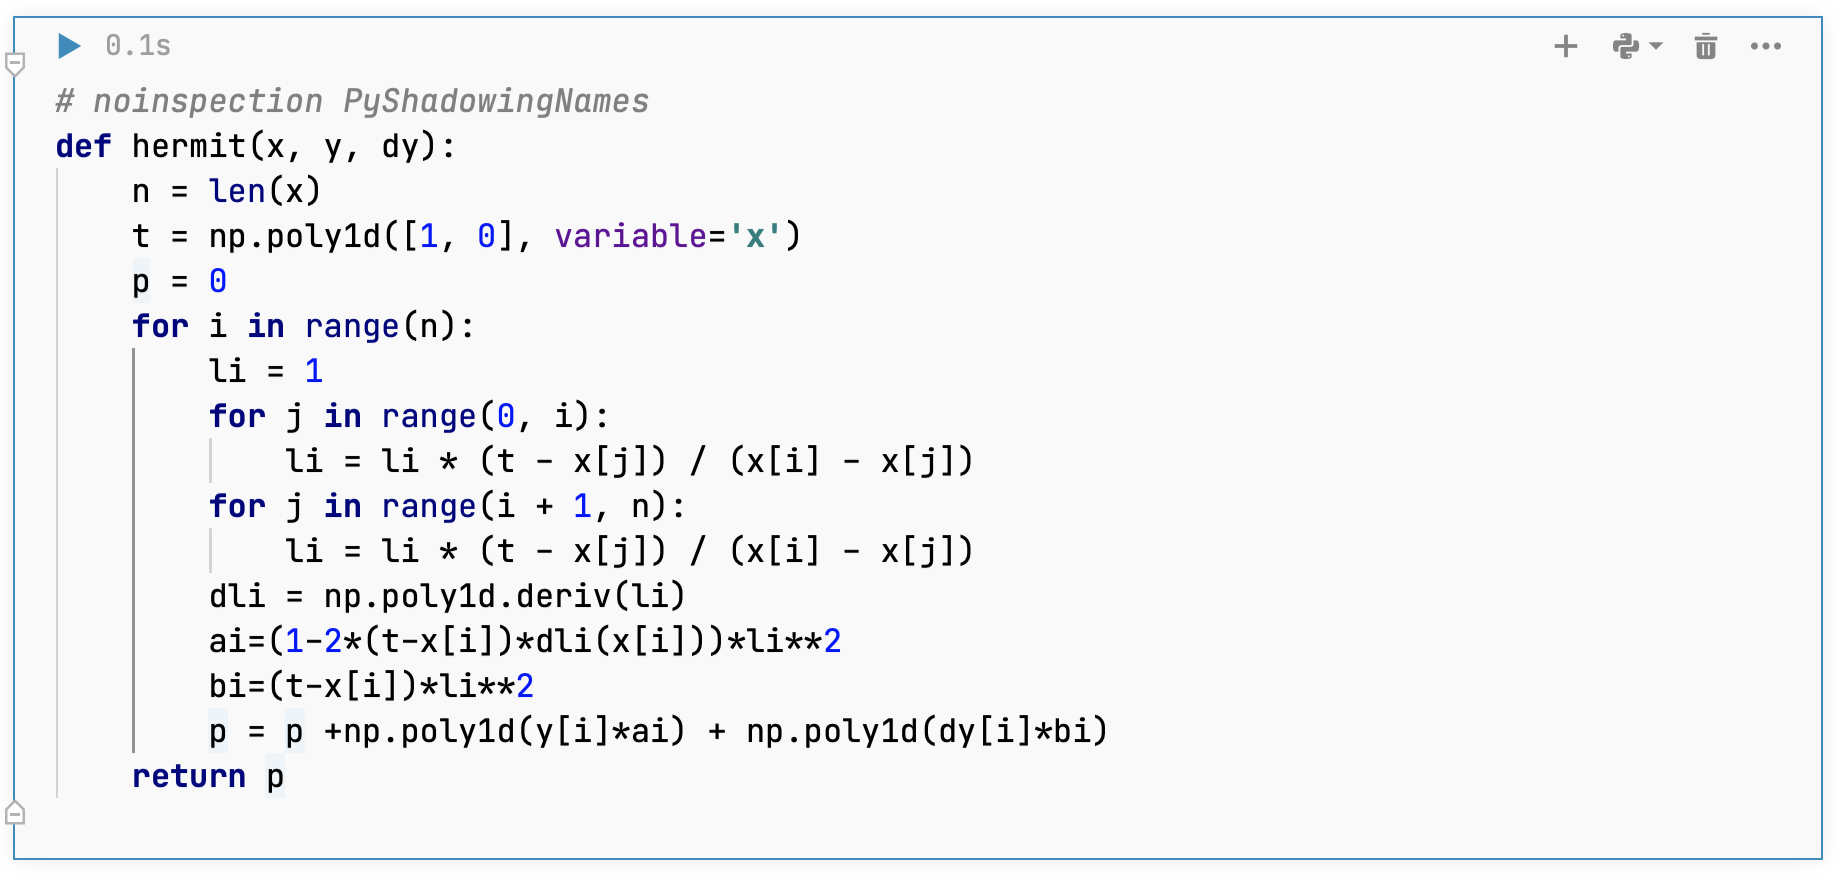
\includegraphics[width=10cm]{images/interpolationDHermit00.png}
\end{center}
\end{frame}

\begin{frame}
 \frametitle{Exemple: $f(x)=1+x\sin x$}
\begin{center}
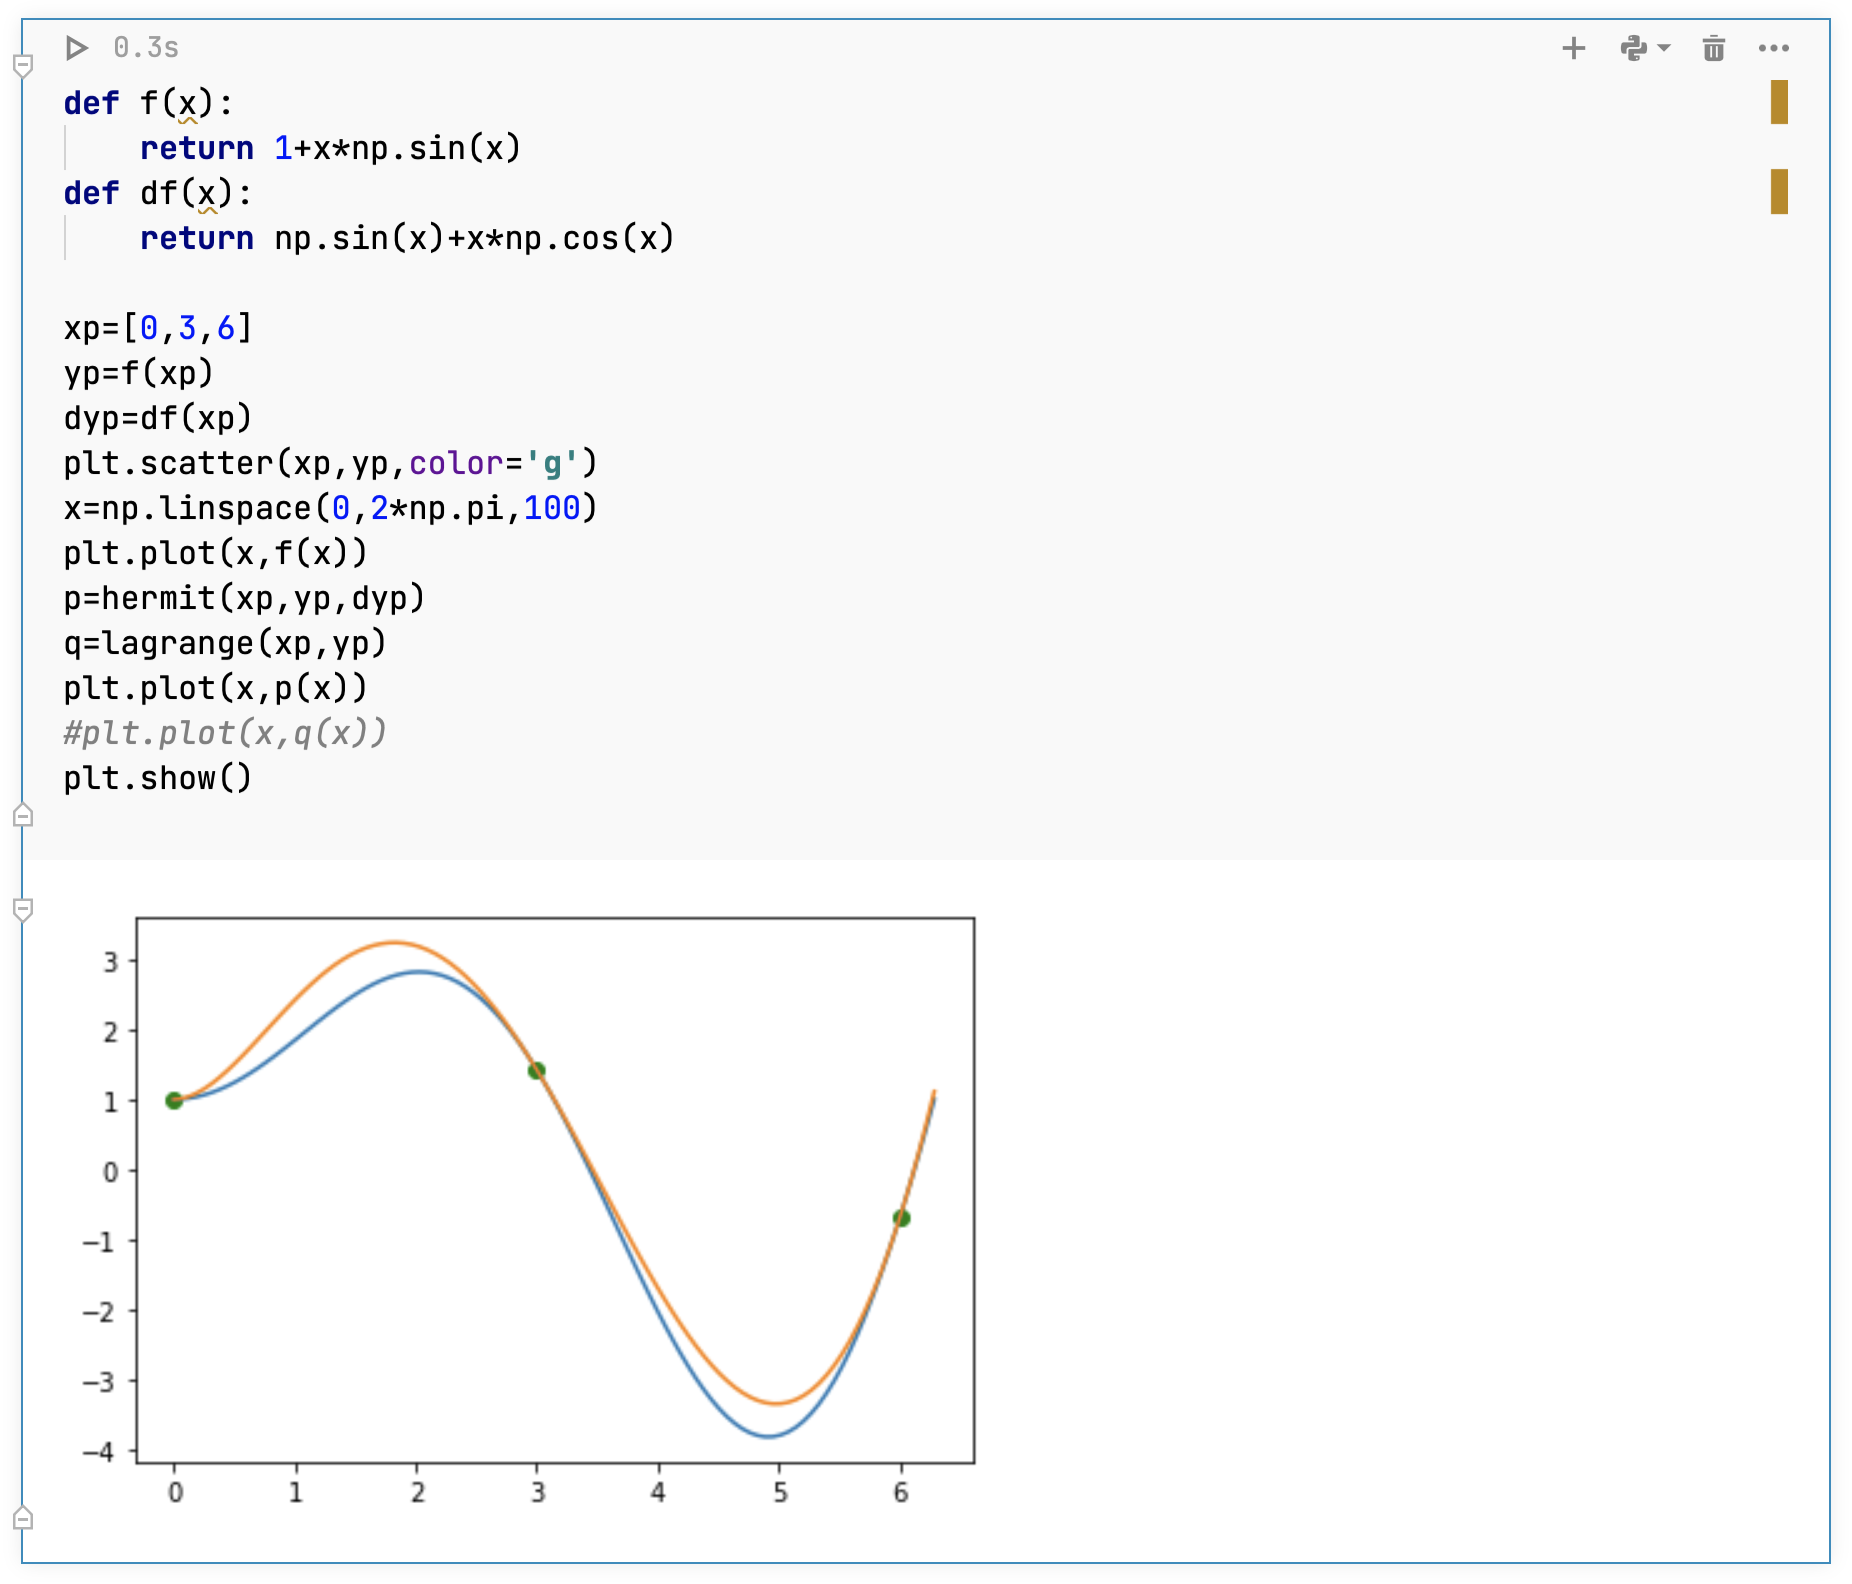
\includegraphics[width=10cm]{images/interpolationDHermite01.png}
\end{center}
\end{frame}

%\begin{frame}
% \frametitle{Exemple}
%\begin{center}
%
%\begin{tikzpicture}[scale=1]
%\draw  [very thin, gray] [->]  (-.2,0) -- (6.5,0); 
%\draw  [very thin, gray] [->] (0,-.2) -- (0,4);
%
%\path[fill=black] (0,1) circle (1.2mm) [fill=gray];
%\path[fill=black]  (3,1.42) circle (1.2mm) [fill=gray];
%\path[fill=black]  (6,-.68) circle (1.2mm) [fill=gray];
%\draw [orange,domain=0:6.2][smooth] plot(\x,{1+\x*sin(\x*180/pi)});
%\draw [domain=0:6][smooth][line width=1][dashed] plot(\x,{-.12831e-1*\x*\x*\x*\x*\x+.25880*\x*\x*\x*\x-1.5521*\x*\x*\x+2.7204*\x*\x+1.});
%
%\end{tikzpicture}  
% 
%\end{center}
%\end{frame}


\begin{frame}
 \frametitle{Exemple: la fonction  $x\mapsto \frac 1{x^2+1}$}
\begin{center}
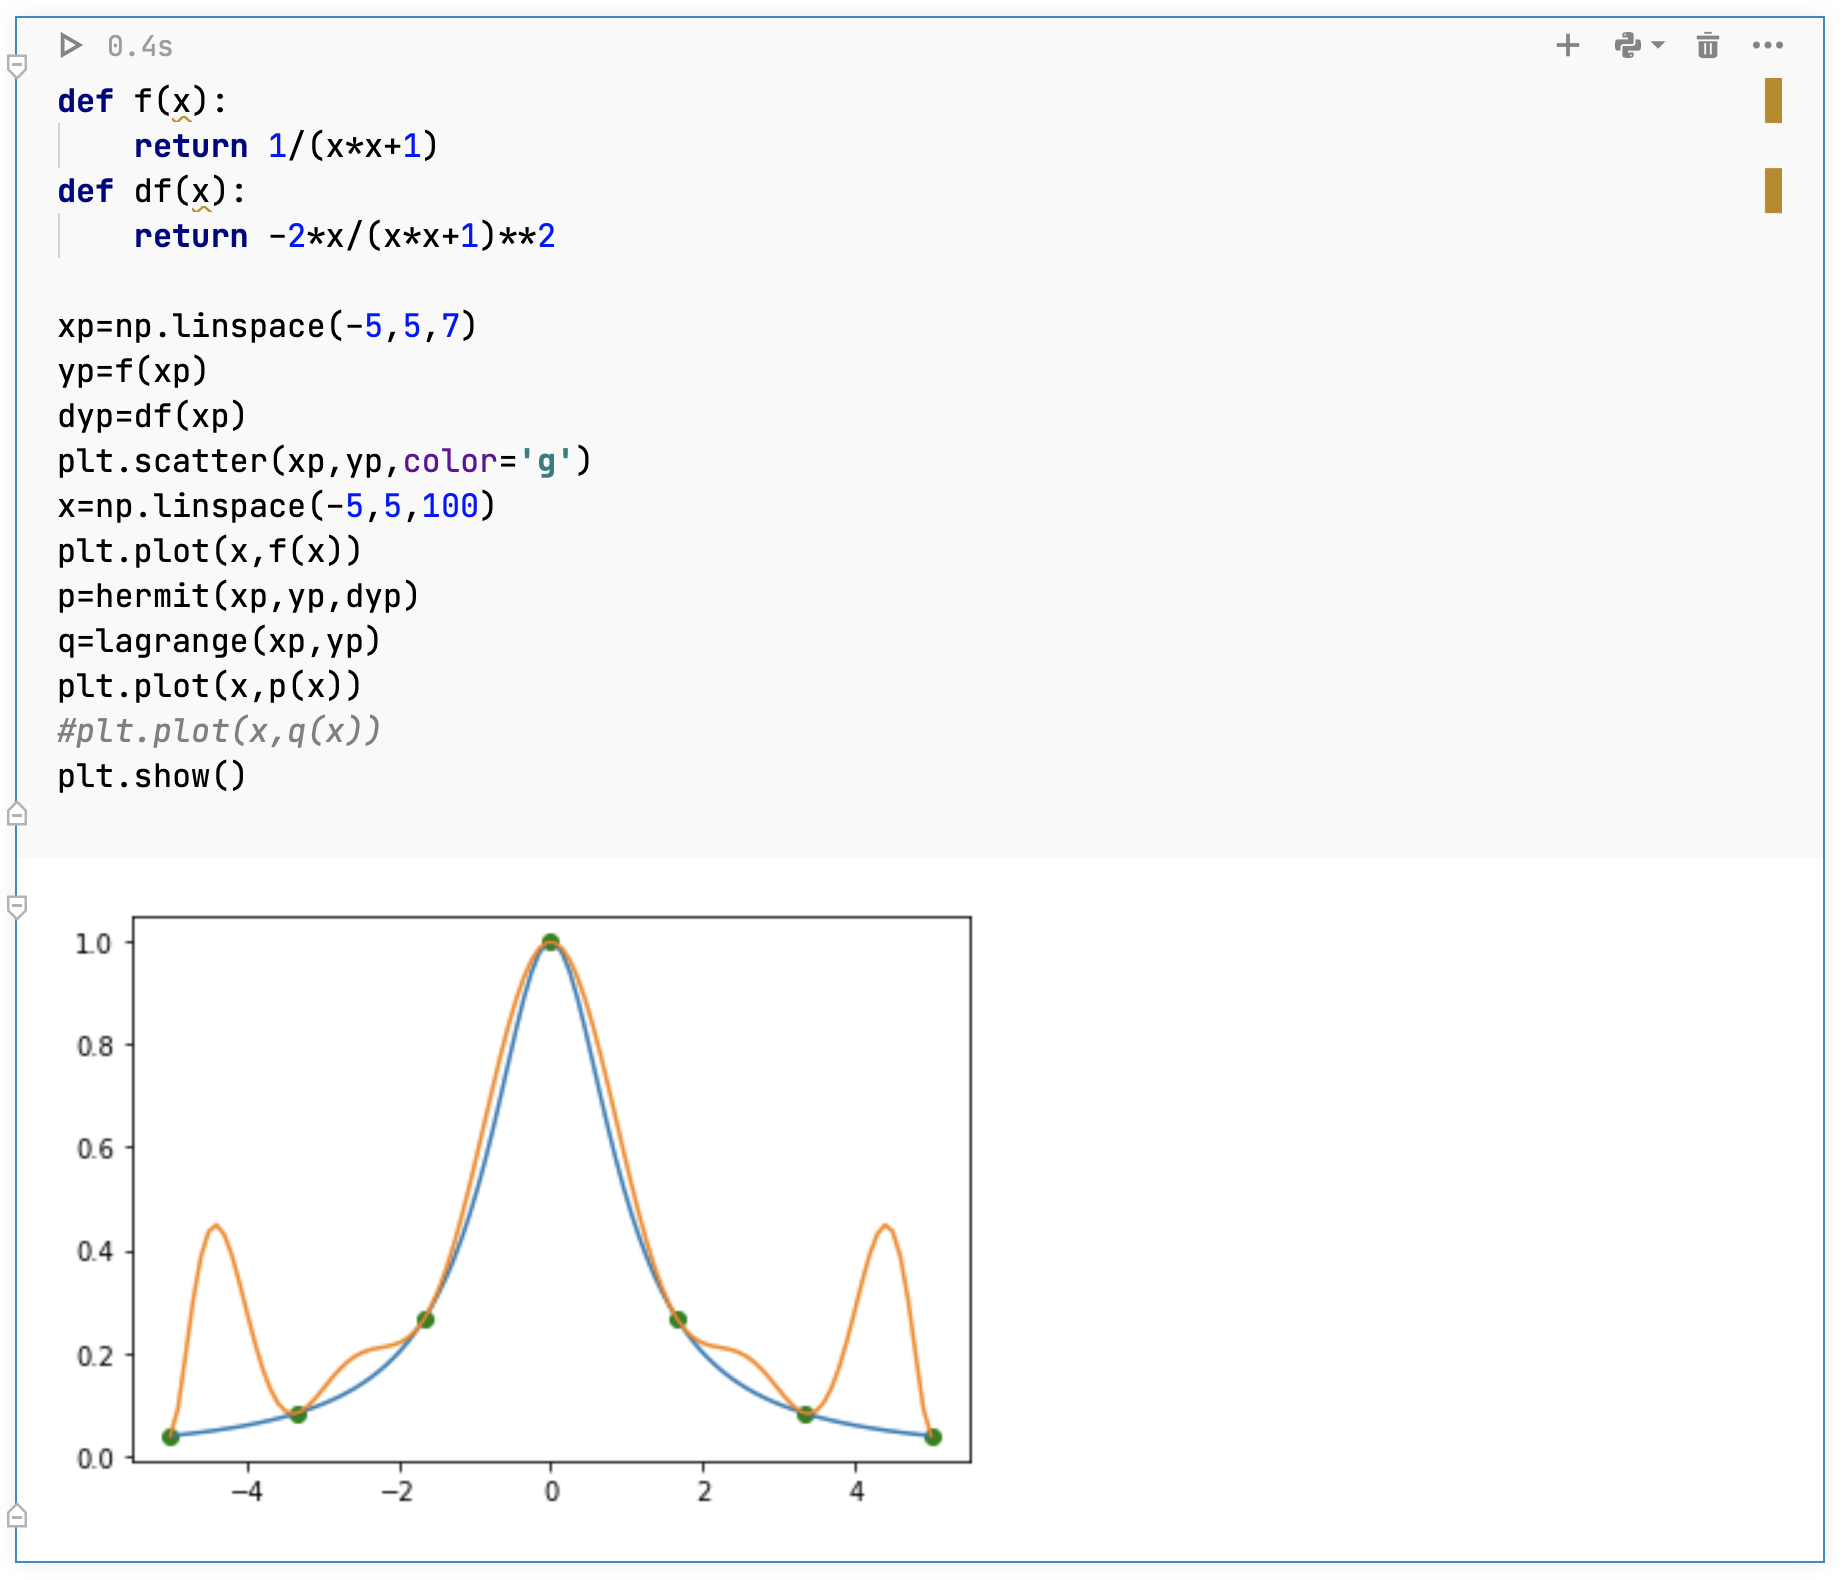
\includegraphics[width=10cm]{images/interpolationDHermite02.png}
\end{center}
\end{frame}

\begin{frame}
\begin{block}{Théorème(Erreur d'interpolation d'Hermite)}
Soit $f \in C^{2n+2}([a, b])$ et $a \leq x_0 < x_1 < x_2 < ... < x_n \leq b$. Soit $P$ le polynôme d'Hermite défini par $P(x_i) = f(x_i)$ et $P'(x_i) = f'(x_i)$ pour $i = 0, 1, ..., n$.
Alors
\[f(x) - P(x) =\frac{L(x)}{(2n + 2)!}f^{(2n+2)}(\xi)\]
où $L(x)=\prod_{i=0}^n\left(x-x_j\right)^2$ et $a < \xi < b$.
\end{block}
Le meilleur choix de $\left(x_i\right)_{i=0,n}$ est alors les racines du polynôme de Tchebychev. 
\end{frame}



\begin{frame}
 \frametitle{Spline linéaire}
 Étant donné  $x_0< x_1 <\cdots < x_n$, on approche $f$ par une
fonction continue qui, sur chaque intervalle $[x_i ,x_{i+1}]$, est définie par le segment joignant les deux points $(x_i , f(x_i ))$ et $(x_{i+1}, f(x_{i+1} ))$. Cette fonction est appelée interpolation linéaire par morceaux (ou spline linéaire)
\begin{block}{Spline linéaire}
 \[\left\{\begin{array}{l}
 \mbox{Pour }x_i<x<x_{i+1}\\
s(x)=f(x_i)+\frac{x-x_i}{x_{i+1}-x_{i}}\left(f(x_{i+1})-f(x_{i})\right)
\end{array}\right.
\]
\end{block}
Erreur
\[\myredbox{\left| f(x) - s(x)\right| \leq \frac 18 M_2 h^2}\]
\end{frame}



\begin{frame}
On considère les points $[0,0],[1,1],[2,4],[3,3]$;
\[\left\{\begin{array}{ll}
 y_0+\frac{y_1-y_0}{x_{1}-x_{0}}\left(x-x_0\right) &\mbox{si } x\in [x_0,x_1]\\
  y_1+\frac{y_2-y_1}{x_{2}-x_{1}}\left(x-x_1\right) &\mbox{si } x\in [x_1,x_2]\\
  y_2+\frac{y_3-y_2}{x_{3}-x_{2}}\left(x-x_2\right) &\mbox{si } x\in [x_2,x_3]\\
  \end{array}\right.
 \]
 d'où
 \[s(x)=\left\{\begin{array}{ll}
 x&\mbox{si } x\in [0,1]\\
 3 x-2 & \mbox{si } x\in [1,2]\\
 -x+6 & \mbox{si } x\in [2,3]
  \end{array}\right.
 \]
  \begin{center}
 \begin{tikzpicture}[scale=0.7]
\draw  [very thin, gray] [->]  (-.1,0) -- (6.2,0); 
\draw  [very thin, gray] [->] (0,-0.1) -- (0,4.5);
\node[gray]  at (0,0) {$\bullet$};\node  at (0,-0.3) {$0$};
\node[gray]  at (2,0) {$\bullet$};\node  at (2,-0.3) {$1$};
\node[gray] at (4,0) {$\bullet$};\node  at (4,-0.3) {$2$};
\node[gray]  at (6,0) {$\bullet$};\node  at (6,-0.3) {$3$};
\path[fill=black] (0,0) circle (1.2mm) [fill=orange];
\path[fill=black]  (2,1) circle (1.2mm) [fill=orange];
\path[fill=black]  (4,4) circle (1.2mm) [fill=orange];
\path[fill=black]  (6,3) circle (1.2mm) [fill=orange];

\draw  [very thin, dashed] (2,0) -- (2,1) -- (0,1);\node  at (-0.3,1) {$1$};
\draw  [very thin, dashed] (4,0) -- (4,4) -- (0,4);\node  at (-0.3,4) {$4$};
\draw  [very thin, dashed] (6,0) -- (6,3) -- (0,3);\node  at (-0.3,3) {$3$};

\draw [gray,domain=0:2][line width=1] plot(\x,\x/2);
\draw [gray,domain=2:4][line width=1] plot(\x,3*\x/2-2);
\draw [gray,domain=4:6][line width=1] plot(\x,-\x/2+6);



\end{tikzpicture} 
 \end{center}
\end{frame}




\begin{frame}
 \frametitle{Spline cubique}
 Étant donné  $x_0< x_1 <\cdots < x_n$, on approche $f$ par une
fonction de classe $C^2$ qui, sur chaque intervalle $[x_i ,x_{i+1}]$, est définie par un polynôme de degré $3$. 
\begin{itemize}
\item Le nombre total d'inconnues est $4 n$
\item Les conditions $s(x_i)=f_i$ imposent $2$ contraintes pour les $n$ polynômes $\Longrightarrow 2 n$ contraintes
\item Les dérivées première et seconde, à gauche et à droite doivent coïncider en chacun de ses $n-1$ points $\Longrightarrow 2(n-1)$ contraintes
\item Deux conditions supplémentaires sont donc nécessaires
\[s'(x_0)\simeq \frac{f(x_1)-f(x_0)}{x_1-x_0}\mbox{ et } s'(x_n)\simeq \frac{f(x_n)-f(x_{n-1})}{x_n-x_{n-1}}\]
\end{itemize}

\end{frame}

\begin{frame}
\begin{center}

 \begin{tikzpicture}[scale=4]
\draw  [very thin, gray] [->]  (-.7,0) -- (2.2,0); 
\draw  [very thin, gray] [->] (-.5,-0.2) -- (-.5,1.5);
\node [blue] at (-0.1,0) {$\bullet$};
\node [blue] at (1,0) {$\bullet$};
\node [blue] at (2,0) {$\bullet$};
\node [blue] at (1,1) {$\circ$};
\path[fill=black] (1,1) circle (0.3mm) [fill=gray];
\path[fill=black]  (-.1,0.616) circle (0.3mm) [fill=gray];
\path[fill=black]  (2,1) circle (0.3mm) [fill=gray];

\draw [orange,domain=-0.1:1][line width=1] plot(\x,6*\x*\x*\x-9*\x*\x+3*\x+1);
\draw [orange,domain=1:2][line width=1] plot(\x,29*\x-13-19*\x*\x+4*\x*\x*\x);
\draw [domain=-0.2:2.2][line width=1] plot(\x,-\x*\x/6+\x/2+2/3);
\draw  [gray] [<->] (0.875,0.625) -- (1.125,1.375);
\draw  [dashed] [<->] (-.1,0.5) -- (0.95,0.5);
\node at (0.5,0.4) {$a_1x^3+b_1x^2+c_1x+d_1$};
\draw  [dashed] [<->] (1.05,0.5) -- (2,0.5);
\node at (1.5,0.4) {$a_2x^3+b_2x^2+c_2x+d_2$};
\end{tikzpicture} 

\end{center}

\end{frame}

\begin{frame}
On considère à nouveau les points $[0,0],[1,1],[2,4],[3,3]$;

 On pose la fonction spline cubique d'interpolation :
  \[s(x)=\left\{\begin{array}{ll}
 f(x)=a_0+a_1x+a_2x^2+a_3x^3 &\mbox{si } x\in [0,1]\\
 g(x)=b_0+b_1x+b_2x^2+b_3x^3 & \mbox{si } x\in [1,2]\\
 h(x)=c_0+c_1x+c_2x^2+c_3x^3& \mbox{si } x\in [2,3]
  \end{array}\right.
 \] 
 Nous avons $3\times 4=12$ inconnues à déterminer.
 \begin{itemize}
 \item La condition $s(x_i)=y_i$ nous donne six équations
 \[f(0)=0, \quad f(1)=1, \quad g(1)=1, \quad g(2)=4, \quad h(2)=4, \quad h(3)=3\]
 
 \[\left\{\begin{array}{l}
                                a_0 = 0\\
                    a_0 + a_1 + a_2 + a_3 = 1\\
                    b_0 + b_1 + b_2 + b_3 = 1\\
                    b_0 + 2 b_1 + 4 b_2 + 8 b_3 = 4\\
                    c_0 + 2 c_1 + 4 c_2 + 8 c_3 = 4\\
                    c_0 + 3 c_1 + 9 c_2 + 27 c_3 = 3\\
 \end{array}\right.
 \]
 
 \end{itemize}
 \end{frame}


\begin{frame}
 
 \begin{itemize}
\item La dérivabilité première nous donne deux équations
 \[f'(1)=g'(1);g'(2)=h'(2);\]
 \[\left\{\begin{array}{l}
    a_1 + 2 a_2 + 3 a_3 = b_1 + 2 b_2 + 3 b_3\\
    b_1 + 4 b_2 + 12 b_3 = c_1 + 4 c_2 + 12 c_3
 \end{array}\right.
 \]    
\item La dérivabilité seconde nous donne aussi deux équations
 \[f''(1)=g''(1);g''(2)=h''(2);\]
  \[\left\{\begin{array}{l}
  2 a_2 + 6 a_3 = 2 b_2 + 6 b_3\\
  2 b_2 + 12 b_3 = 2 c_2 + 12 c_3
 \end{array}\right.
 \]                 
\item Pour que la résolution soit possible, nous imposons deux conditions aux extrémités
 \[f''(0)=0, \qquad h''(3)=0\]
\[\left\{\begin{array}{l}
 2 a_2 = 0\\
 2 c_2 + 18 c_3 = 0
 \end{array}\right.
 \]  

 
 \end{itemize}
 
 
\end{frame}


\begin{frame} 
 
 Nous avons bien 12 équations à 12 inconnues d'où la solution
 \[s(x)=\left\{\begin{array}{ll}
 \frac 45 x^3+\frac 15 x&\mbox{si } x\in [0,1]\\
 -2x^3+\frac{42}5 x^2-\frac{41}5 x +\frac{14}5 & \mbox{si } x\in [1,2]\\
 \frac 65 x^3-\frac{54}5 x^2+\frac{151}5 x -\frac{114}5& \mbox{si } x\in [2,3]
  \end{array}\right.
 \]
 
 \begin{center}
 \begin{tikzpicture}[scale=1]
\draw  [very thin, gray] [->]  (-.1,0) -- (6.2,0); 
\draw  [very thin, gray] [->] (0,-0.1) -- (0,4.5);
\node  at (0,0) {$\bullet$};\node  at (0,-0.3) {$0$};
\node  at (2,0) {$\bullet$};\node  at (2,-0.3) {$1$};
\node at (4,0) {$\bullet$};\node  at (4,-0.3) {$2$};
\node  at (6,0) {$\bullet$};\node  at (6,-0.3) {$3$};
\path[fill=black] (0,0) circle (1.2mm) [fill=gray];
\path[fill=black]  (2,1) circle (1.2mm) [fill=gray];
\path[fill=black]  (4,4) circle (1.2mm) [fill=gray];
\path[fill=black]  (6,3) circle (1.2mm) [fill=gray];

\draw  [very thin, dashed] (2,0) -- (2,1) -- (0,1);\node  at (-0.3,1) {$1$};
\draw  [very thin, dashed] (4,0) -- (4,4) -- (0,4);\node  at (-0.3,4) {$4$};
\draw  [very thin, dashed] (6,0) -- (6,3) -- (0,3);\node  at (-0.3,3) {$3$};

\draw [orange,domain=0:2][line width=1] plot(\x,1/10*\x+1/10*\x*\x*\x);
\draw [orange,domain=2:4][line width=1] plot(\x,14/5-41/10*\x+21/10*\x*\x-1/4*\x*\x*\x);
\draw [orange,domain=4:6][line width=1] plot(\x,-114/5+151/10*\x-27/10*\x*\x+3/20*\x*\x*\x);

\end{tikzpicture} 
 \end{center}
\end{frame}
\begin{frame}
 \frametitle{Splines cubiques : détermination}
 \begin{itemize}
 \item $s$ coïncide sur chaque intervalle $[x_i; x_{i+1}]$ avec un polynôme de
degré inférieur ou égal à 3
\item $s''$ est de degré 1 et est déterminé par 2 valeurs (moment au nœud $i$):
\[m_i = s''(x_i) \mbox{ et } m_{i+1} = s''(x_{i+1}) \]
\item Notations :
\begin{itemize}
\item  $h_i = x_{i+1} - x_i$ pour $i = 0 … n-1$
\item  $ \delta_i=[x_i; x_{i+1}]$ 
\item   $s_i(x)$ le polynôme de degré 3 qui coïncide avec $g$ sur l'intervalle $ \delta_i$ 
\end{itemize}
 \end{itemize}
 \end{frame}
 
 \begin{frame}
 \begin{itemize}
\item $s''_i(x)$ est linéaire :
 \begin{itemize}
\item \[\forall x\in \delta_i,\quad s''(x)=-m_{i} \frac{x-x_{i+1}}{h_i}+m_{i+1} \frac{x-x_{i}}{h_i}\]
\item on intègre 
\[\forall x\in \delta_i,\quad  s'(x)=-m_{i} \frac{(x-x_{i+1})^2}{2h_i}+m_{i+1} \frac{(x-x_{i})^2}{2h_i}+a_i\]
\item on continue
\[\forall x\in \delta_i,\quad  s(x)=-m_{i} \frac{(x-x_{i+1})^3}{6h_i}+m_{i+1} \frac{(x-x_{i})^3}{6h_i}+a_i(x-x_i)+b_i\]
\end{itemize}
\item continuité de $s_i$ en $x_i$
\[s_i(x_i)=y_i \Longrightarrow \myredbox{y_i=\frac{m_i h_i^2}{6}+b_i}\]
\item continuité de $s_i$ en $x_{i+1}$
\[s_i(x_{i+1})=y_{i+1} \Longrightarrow \myredbox{ y_{i+1}=\frac{m_{i+1} h_i^2}{6}+a_ih_i+b_i}\]
\end{itemize}
\end{frame}

\begin{frame}
 \frametitle{Splines cubiques : détermination}
 
 \begin{itemize}
 \item Éliminons $b_i$:
 \[a_i=\frac 1{h_i}\left(y_{i+1}-y_i\right)-\frac {h_i}6\left(m_{i+1}-m_i\right)\]
 \item continuité de $s'(x_i)$:
 \[s'_i(x_i)=-m_i\frac{h_i}{2}+a_i=-m_i\frac{h_{i-1}}{2}+a_{i-1}=s'_{i-1}(x_i)\]
 \item Éliminons $a_i$:
 \[\myredbox{ h_{i-1}m_{i-1}+2(h_i+h_{i-1})m_i+h_i m_{i+1}=6\left(\frac {y_{i+1}-y_i}{h_i}-\frac {y_{i}-y_{i-1}}{h_{i-1}}\right)}\]
\end{itemize}
\end{frame}

\begin{frame}

on cherche les $m_i$ ($n+1$ inconnues)
\begin{itemize}
 \item on a seulement $n-1$ équations
 \item il faut rajouter 2 conditions, par exemple (spline naturelle)
 \[m_0=m_n=0\]
 \item cas où le pas $h_i$ est constant:
 \[\myredbox{ m_{i-1}+4m_i+m_{i+1}=\frac 6{h^2}\left(y_{i-1}-2y_i+y_{i+1}\right)} \mbox{ pour }i=1,n-1\]
\end{itemize}
La matrice du système est symétrique définie positive:
\[\left(\begin{array}{ccccc}
4 & 1 & &&\\
1 & 4 & 1 &&\\
 & \ddots & \ddots &\ddots&\\
&& 1 & 4 & 1 \\
&& & 1 & 4
\end{array}\right)
\]

\end{frame}


\begin{frame}
 \frametitle{Code python}
\begin{center}
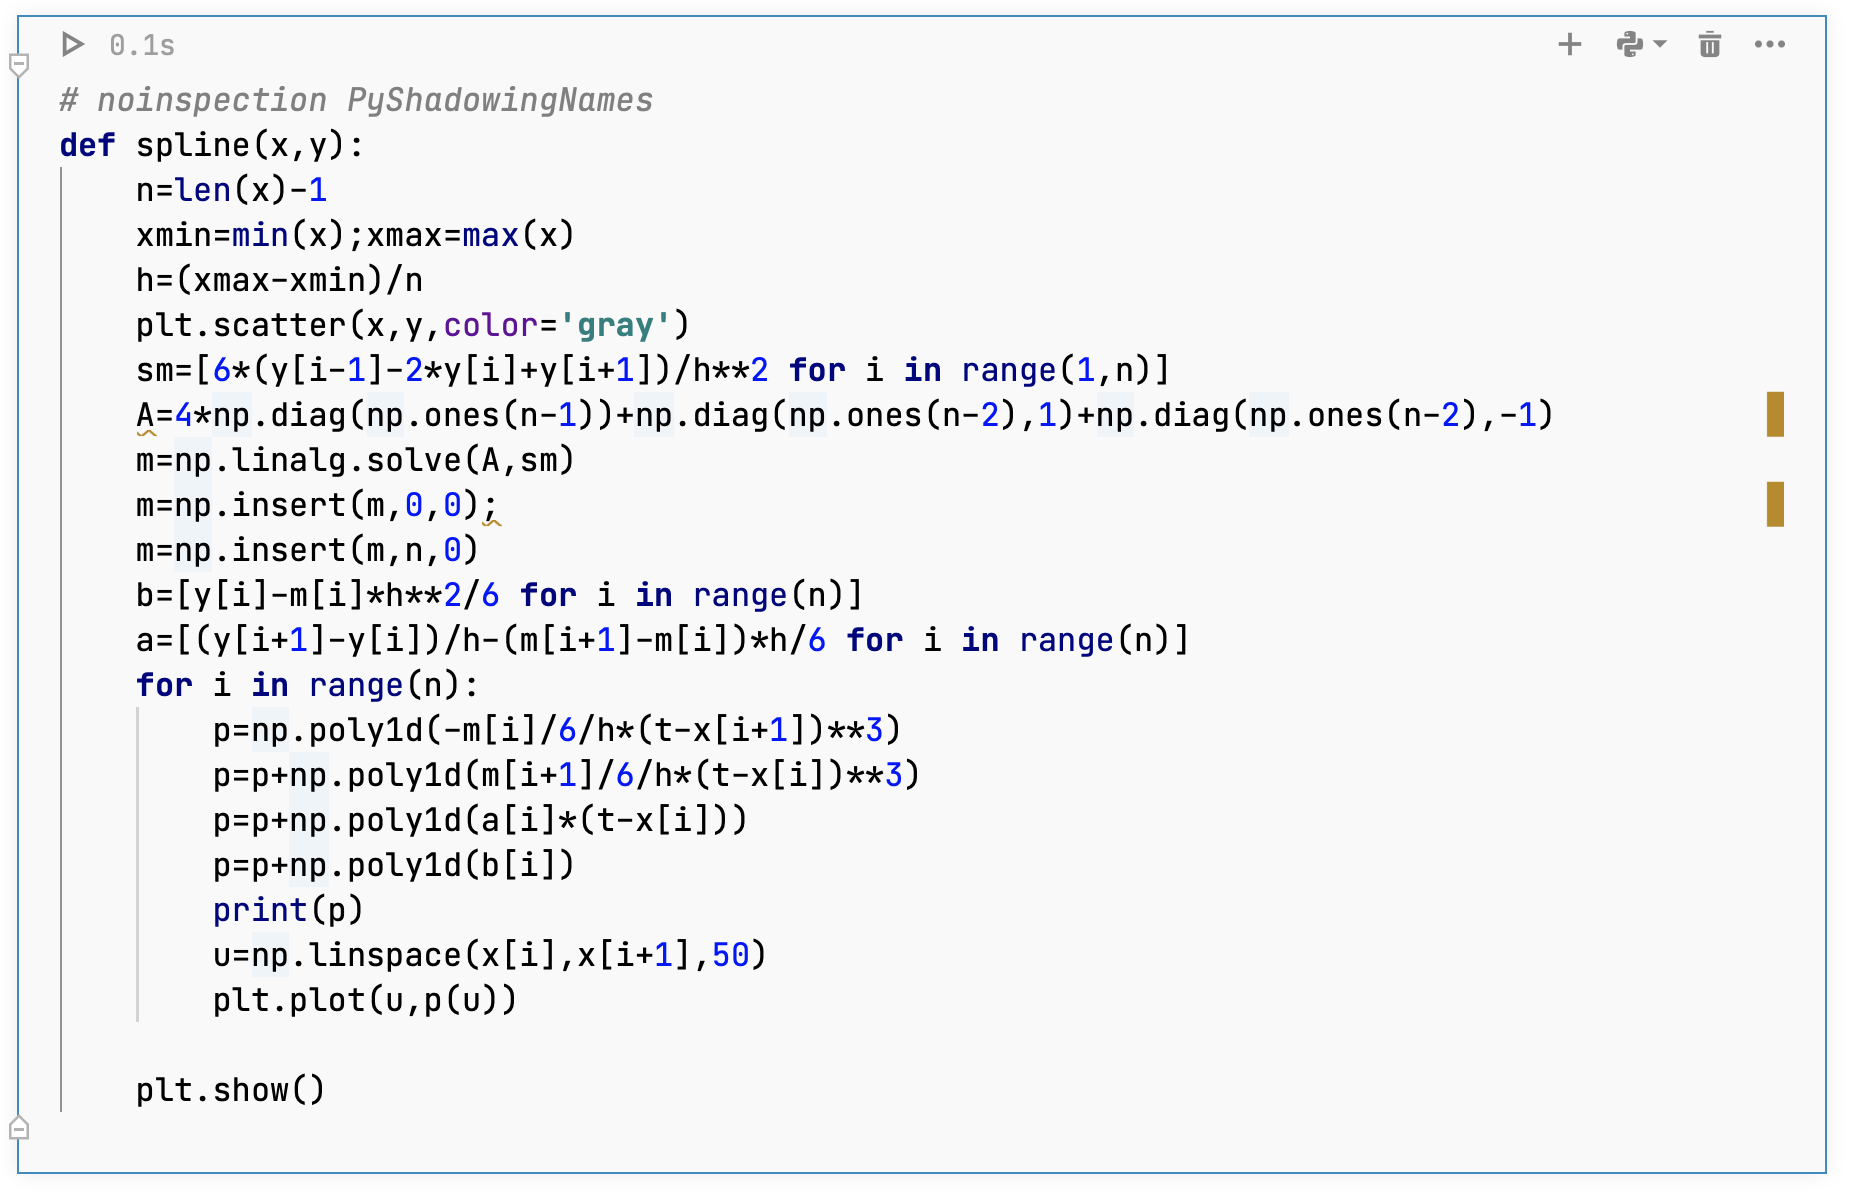
\includegraphics[width=10cm]{images/interpolationDHermite03.png}
\end{center}
\end{frame}

\begin{frame}
 \frametitle{Exemple}
\begin{center}
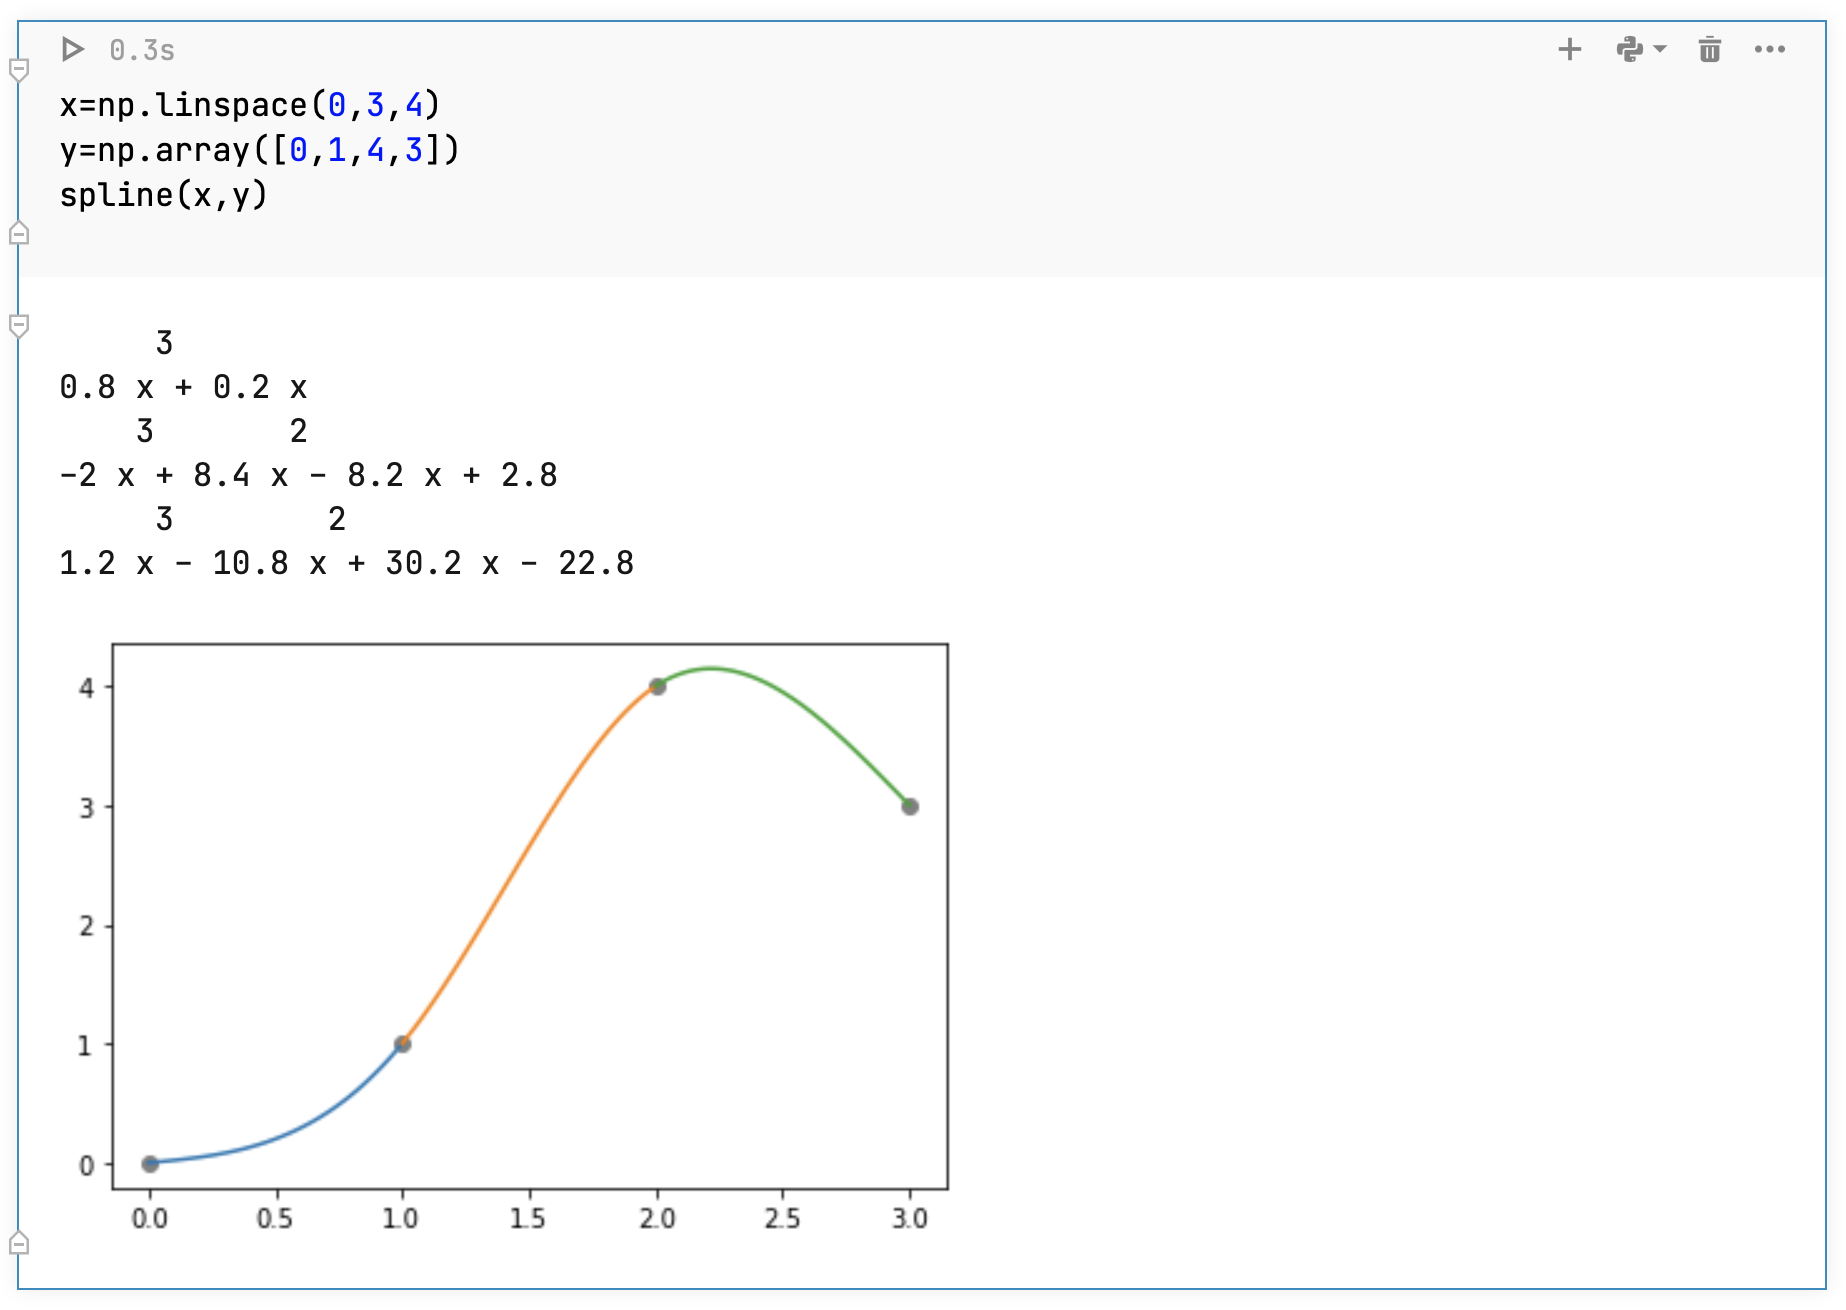
\includegraphics[width=10cm]{images/interpolationDHermite04.png}
\end{center}
\end{frame}

\begin{frame}
 \frametitle{Exemple}
Interpolation par spline cubique de $f:x\mapsto \frac 1{x^2+1}$ sur l'intervalle $[-5,5]$ en 9 points: on applique la méthode à la suite de points
 \[\left(\left[-5+10\times \frac k8,f\left(-5+10\times \frac k8\right)\right]\right)_{k=0,1,..,8}\]
 
 \begin{center}
 \begin{tikzpicture}[yscale=1]
\draw  [very thin, gray] [->]  (-5,0) -- (5,0); 
\draw  [very thin, gray] [->] (0,-0.1) -- (0,4.5);
\node[gray]  at (-5,0) {$\bullet$};
\node[gray]  at (-3.75,0) {$\bullet$};
\node[gray] at  (-2.50,0) {$\bullet$};
\node[gray]  at (-1.25,0) {$\bullet$};
\node[gray]  at (5,0) {$\bullet$};
\node[gray] at (3.75,0) {$\bullet$};
\node [gray] at  (2.50,0) {$\bullet$};
\node[gray]  at (1.25,0) {$\bullet$};
\node[gray]  at (0,0) {$\bullet$};

\path[fill=black] (-5,4*.385e-1) circle (0.7mm) [fill=green];
\path[fill=black]  (-3.75,4*.664e-1) circle (0.7mm) [fill=green];
\path[fill=black]  (-2.50,4*.138) circle (0.7mm) [fill=green];
\path[fill=black]  (-1.25,4*.390) circle (0.7mm) [fill=green];
\path[fill=black]  (0,4*1) circle (0.7mm) [fill=green];
\path[fill=black] (5,4*.385e-1) circle (0.7mm)[fill=green];
\path[fill=black]  (3.75,4*.664e-1) circle (0.7mm) [fill=green];
\path[fill=black]  (2.50,4*.138) circle (0.7mm) [fill=green];
\path[fill=black]  (1.25,4*.390) circle (0.7mm) [fill=green];

\draw [orange,domain=-5:-3.75][line width=1] plot(\x,{4*(.888+.485*\x+.945e-1*\x*\x+.630e-2*\x*\x*\x)});
\draw [orange,domain=-3.75:-2.50][line width=1] plot(\x,{4*(.730e-1-.167*\x-.794e-1*\x*\x-.916e-2*\x*\x*\x});
\draw [orange,domain=-2.50:-1.25][line width=1] plot(\x,{4*(1.79+1.89*\x+.744*\x*\x+.101*\x*\x*\x});
\draw [orange,domain=-1.25:0][line width=1] plot(\x,{4*(1-.769*\x*\x-.303*\x*\x*\x});
\draw [orange,domain=0:1.25][line width=1] plot(\x,{4*(1-.769*\x*\x+.303*\x*\x*\x});
\draw [orange,domain=1.25:2.50][line width=1] plot(\x,{4*(1.79-1.89*\x+.744*\x*\x-.101*\x*\x*\x});
\draw [orange,domain=2.50:3.75][line width=1] plot(\x,{4*(.730e-1+.167*\x-.794e-1*\x*\x+.916e-2*\x*\x*\x});
\draw [orange,domain=3.75:5][line width=1] plot(\x,{4*(.888-.485*\x+.945e-1*\x*\x-.630e-2*\x*\x*\x});
\draw [blue,domain=-5:5][smooth] plot(\x,{4/(\x*\x+1)});
\end{tikzpicture}  
 
\end{center} 
 \end{frame}

\begin{frame}
 \frametitle{Exemple}
\begin{center}
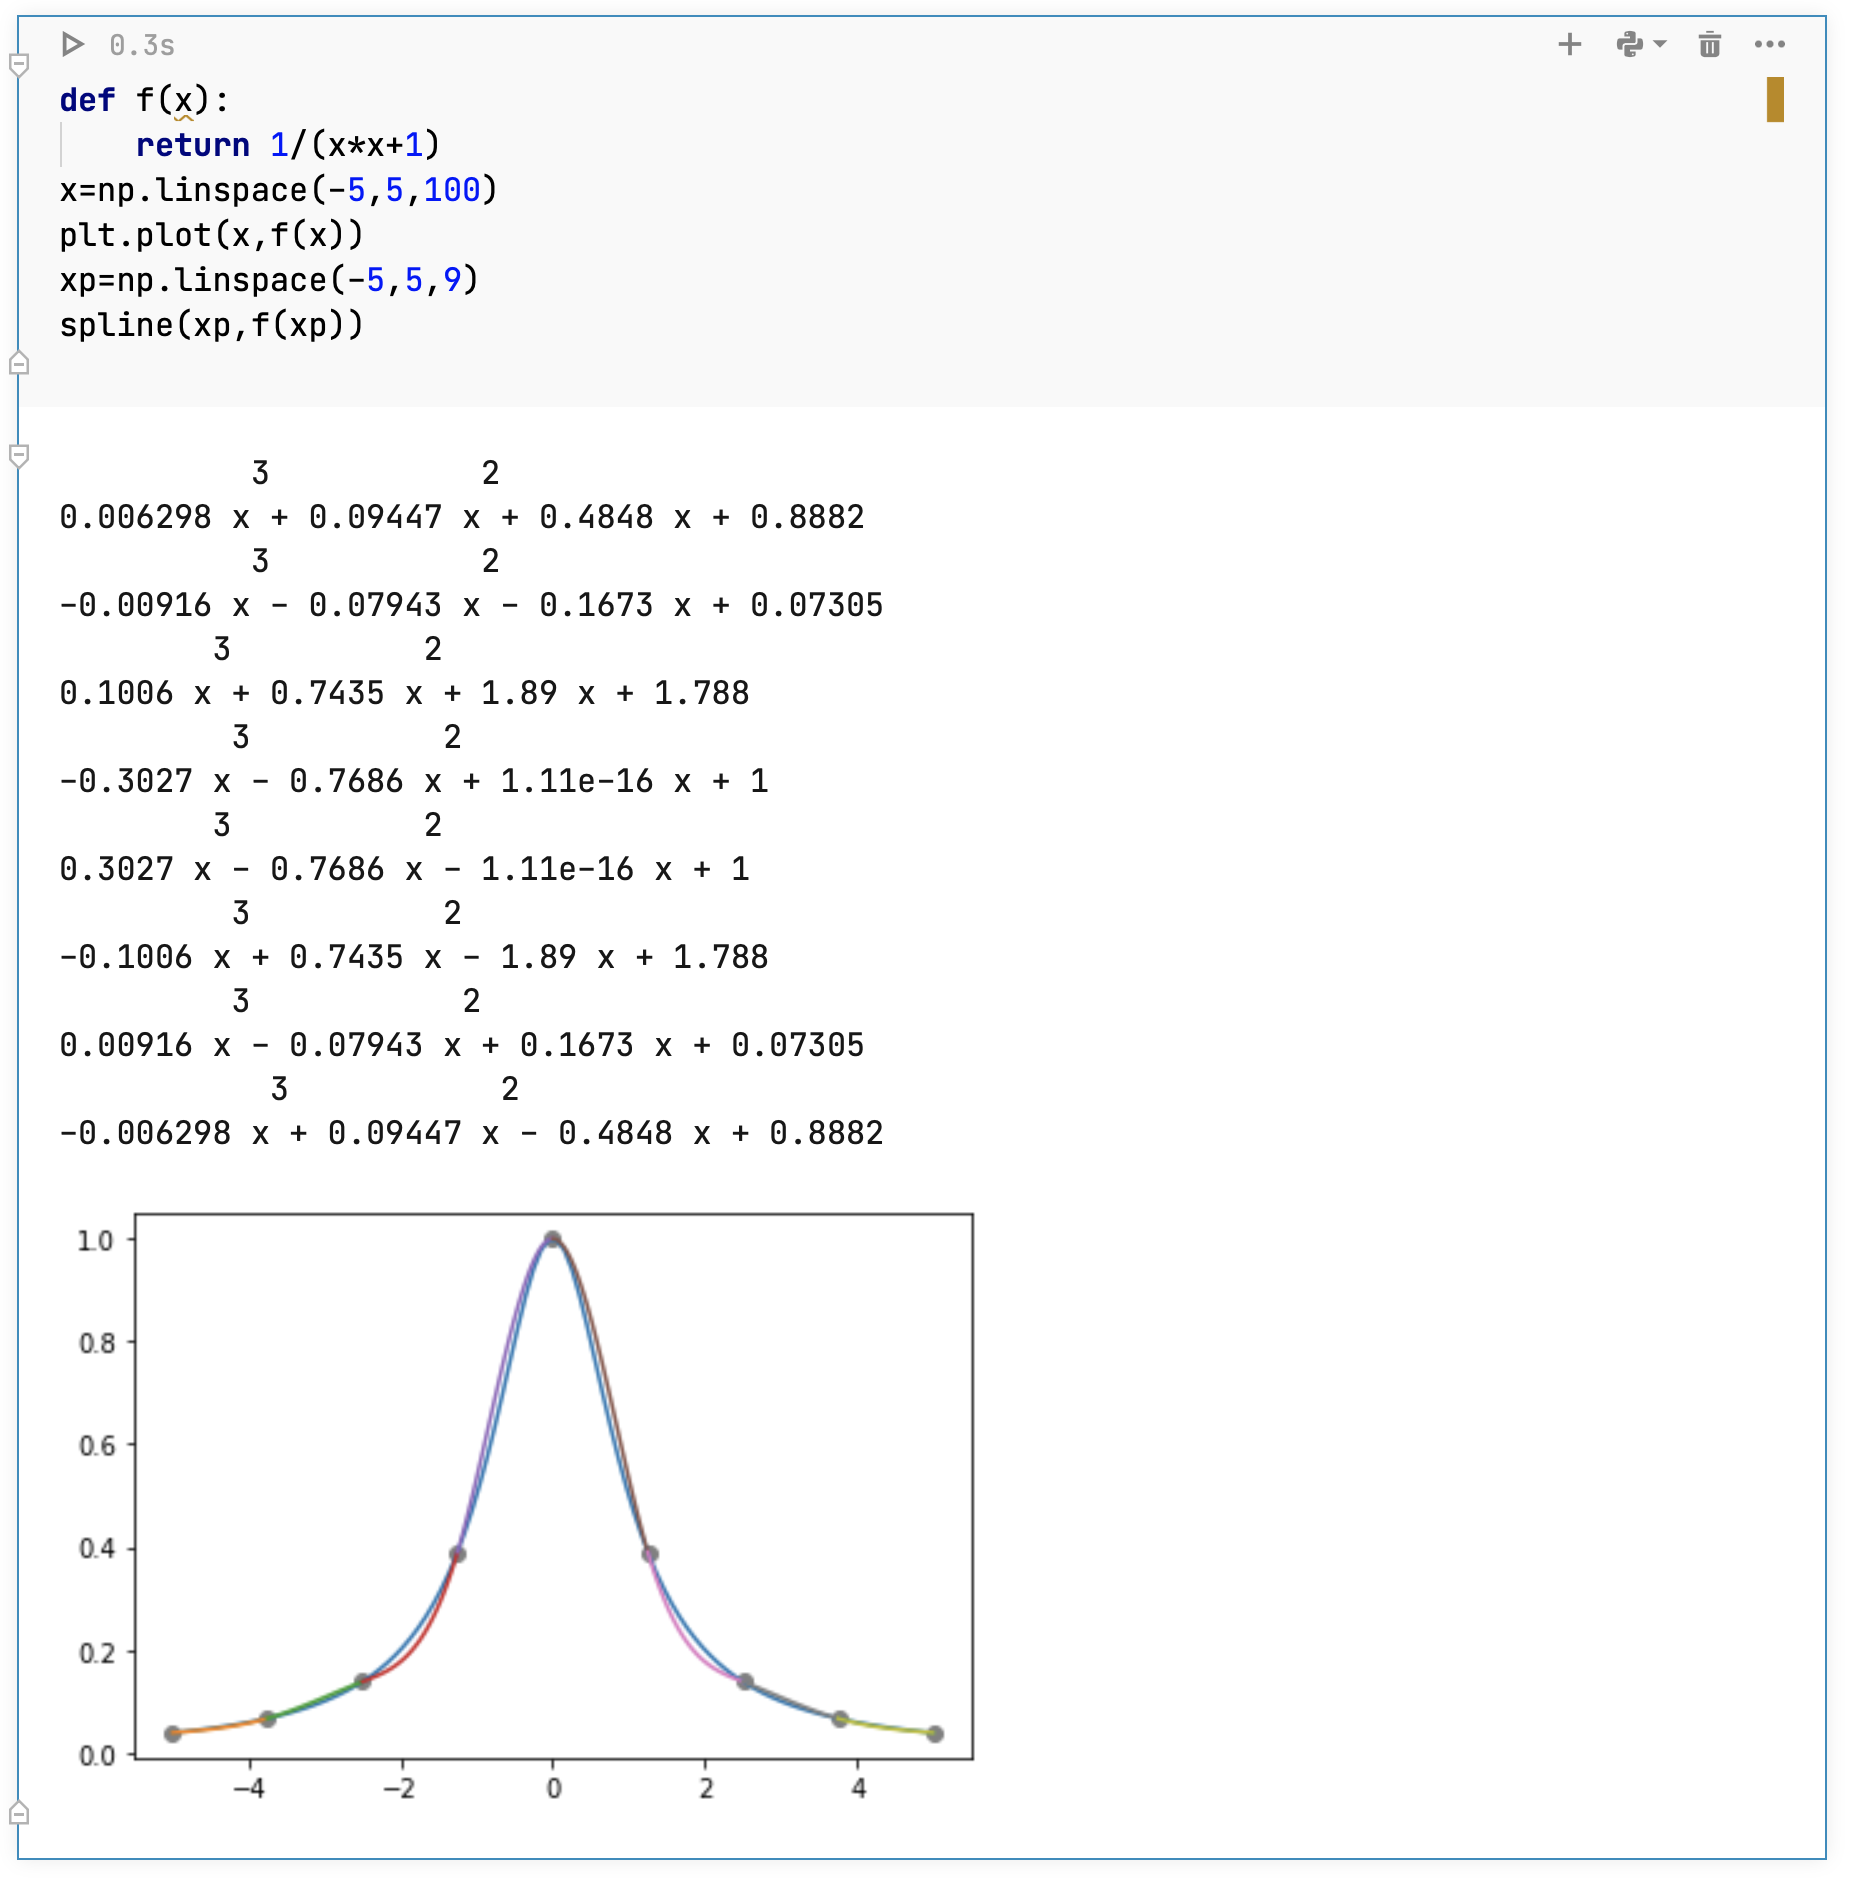
\includegraphics[width=8cm]{images/interpolationDHermite05.png}
\end{center}
\end{frame}

\begin{frame}
 \frametitle{Meilleure approximation}
Soit $V$ un espace vectoriel muni d'un produit scalaire $(\cdot, \cdot)$ et $\|\cdot\|$ la norme associée.
Soit $V_h$ un sous espace de $V$ de dimension finie et $(q_1, q_2, \cdots, q_N)$ une base.

On dit que $u \in V_h$ réalise la meilleure approximation de $f \in V$ ssi $u$ est la projection orthogonale de $f$ sur $V_h$:
\[ d(f,V_h)=\|f-u\|=\min_{v\in V_h}\|f-v\| \]

\begin{center}
 \begin{tikzpicture}[domain=0:5]
  \filldraw  [gray!20,draw opacity=0.5](0,0) -- ++(4,0)-- ++(1.5,2)--++(-4,0)--++(-1.5,-2) ;
  \draw[->] (2,1) -- ++(2,2)node[above]{$\scriptstyle f$}  ;
  \draw[red,->] (2,1) -- ++(2,0.2)node[right]{$\scriptstyle u$}  ;
   \draw[blue,dotted] (4,1.2) -- (4,3);
  \draw[->] (2,1) -- ++(1,-0.5)node[below]{$\scriptstyle q_1$} ;
  \draw[->] (2,1) -- ++(1.25,-0.25) node[right]{$\scriptstyle q_2$};
  \draw[->] (2,1) -- ++(1,0.25)node[above]{$\scriptstyle q_n$} ;
 
  \draw (0.5,0.25)  node{$\scriptstyle V_h$};
 
\end{tikzpicture}
 \end{center}



\end{frame}

\begin{frame}
Si $u=\sum_{i=0}^N \lambda_i^* q_i$ alors $\lambda^*=(\lambda^*_i)_{i=0,N}$ réalise le minimum de la fonctionnel quadratique 
\[J(\lambda)=\|\sum_{i=0}^N \lambda_i q_i-f\|^2\]
Le développement de $J$:
\[J(\lambda)=\sum_{i,j=0}^N \lambda_i \lambda_j(q_i,q_j)-2\sum_{i=0}^N \lambda_i(f,q_i)+\|f\|^2\]
s'écrit
\[\myredbox{J(\lambda)=<A\lambda,\lambda>-2<b,\lambda>+\|f\|^2}\]

où $A=\left[(q_i,q_j)\right]_{ij}$ est une matrice symétrique définie positive, et $b=(f,q_i)_i$ un vecteur dépendant de $f$ et de la base choisie. 


\end{frame}


\begin{frame}

Soit $\lambda$ et $\varepsilon$ deux vecteurs de $V_h$, nous avons
\[ \begin{array}{ccl}
J(\lambda+\varepsilon)&=&<A(\lambda+\varepsilon),\lambda+\varepsilon> -2<b,\lambda+\varepsilon>+\|f\|^2 \\
&=&<A\lambda,\lambda>+<A\lambda,\varepsilon>+<A\varepsilon,\lambda>+<A\varepsilon,\varepsilon>\\
&&-2<b,\lambda> -2<b,\varepsilon>+\|f\|^2 \\
&=&J(\lambda)+2<A\lambda-b,\varepsilon>+<A\varepsilon,\varepsilon>
\end{array}
\]
D'où la dérivée de la fonctionnelle $J$
\[J'(\lambda)=2\left(A\lambda-b\right)\]
$A$ étant définie positive et pour tout $\varepsilon\in V_h$, $<A\varepsilon,\varepsilon>$ est strictement positif et par conséquence $J$ est minimale en $\lambda^*$ tel que 
\[ A\lambda^*=b\]

 
\[\myredbox{ J'(\lambda^*)=0 \Longleftrightarrow A\lambda^*=b}\]

\end{frame}


\begin{frame}
\frametitle{Exemple}
Soit $V = L^2(0, 1)$ muni du produit scalaire $(f, g) =\int_0^1f(x)g(x) dx$. 
 \begin{center}
 \begin{tikzpicture}[domain=0:5]
  \draw[->] (-0.1,0) -- (6.1,0)  node[right] {$\scriptstyle x$};
  \draw[->] (0,-0.1) -- (0,1.5) node[above] {$\scriptstyle y$};
  \path[fill=black]  (0,0) circle (.4mm) [fill=gray] node[below] {$\scriptstyle 0$};
 \path[fill=black]  (0,0) circle (.4mm) [fill=gray];
 \path[fill=black]  (1,0) circle (.4mm) [fill=gray];
 \path[fill=black]  (2,0) circle (.4mm) [fill=gray] node[below] {$\scriptstyle x_{i}$};
  \draw[orange] (0,0.02) -- ++(2,0);
  \draw[orange,dotted] (2,0) -- ++(0,1);
  \draw[orange] (2,1) -- ++(1,0) node[right] {$\scriptstyle q_{i}$};
   \draw[orange,dotted] (3,0) -- ++(0,1);
    \draw[orange] (3,0.02) -- ++(2,0);
 \path[fill=black]  (3,0) circle (.4mm) [fill=gray];
   \draw  (4.5,0.5) node {$\scriptstyle h=\frac 1N$};
   \draw[<->] (4,0.2) -- ++(1,0) ;
   \path[fill=black]  (4,0) circle (.4mm) [fill=gray];
    \path[fill=black]  (5,0) circle (.4mm) [fill=gray] node[below] {$\scriptstyle 1$};

\end{tikzpicture}
 \end{center}
 Soit $V_h = \{v \in V ; v|_{I_k} =\mbox{ constante}\}$. On cherche à calculer la meilleur approximation d'une fonction donnée $f$ dans le sous-espace $V_h$.
 \begin{itemize}
 \item $V_h$ est un espace vectoriel de dimension $N$.
 \item la famille des fonctions caractéristique de $[x_i,x_{i+1}]$, $(q_{k})_{k=0,N-1}$, constitue une base de $V_h$.
 \item la meilleur approximation est un élément de $V_h$ solution de $A\lambda^* = b$
 \end{itemize}                                                        

Les coefficients de la matrice $A$ sont
\[a_{i,j} = (q_i, q_j) =\int_0^1q_i(x)q_j(x) \de x =\left\{\begin{array}{l}
\int_{x_i}^{x_{i+1}}1\times 1 \de x=h \mbox{ si }i=j\\
0 \mbox{ sinon }
\end{array}\right.
\]

\end{frame}

\begin{frame}
ainsi $A = h I$ ($I$ la matrice identité) donc $\lambda^*=\frac 1h b$ où $b$ est le vecteur de $V_h$ donné par
\[b=\sum_{k=1}^N(f,q_k)q_k\]
avec $(f,q_k)=\int_{x_i}^{x_{i+1}}f(x) \de x$. Donc la meilleur approximation de $f$ dans $V_h$ est la fonction en escalier constante sur chaque intervalle de la subdivision dont la constante est la valeur de la moyenne de $f$ sur cet intervalle $\frac 1h \int_{x_i}^{x_{i+1}}f(x) \de x$.

\begin{center}
 \begin{tikzpicture}[domain=0:5]
  \draw[->] (-0.1,0) -- (6.1,0)  node[right] {$\scriptstyle x$};
  \draw[->] (0,-0.1) -- (0,1.5) node[above] {$\scriptstyle y$};
  \path[fill=black]  (0,0) circle (.4mm) [fill=gray] node[below] {$\scriptstyle 0$};
 \path[fill=black]  (0,0) circle (.4mm) [fill=gray];
 \path[fill=black]  (1,0) circle (.4mm) [fill=gray];
 \path[fill=black]  (2,0) circle (.4mm) [fill=gray] node[below] {$\scriptstyle x_{i}$};
 \path[fill=black]  (3,0) circle (.4mm) [fill=gray];
   \draw  (2.5,0.5) node {$\scriptstyle h=\frac 1N$};
   \draw[<->] (2,0.2) -- ++(1,0) ;
   \path[fill=black]  (4,0) circle (.4mm) [fill=gray];
    \path[fill=black]  (5,0) circle (.4mm) [fill=gray] node[below] {$\scriptstyle 1$};
\draw [domain=0:5][line width=0.5] plot(\x,{(1/3*\x*\x*\x-3*\x*\x+8*\x)/3});
 \draw[orange] (0,1.03) -- ++(1,0)-- ++(0,1.05)-- ++(1,0)--++(0,0.06)--++(1,0)--++(0,-0.28)--++(1,0)--++(0,0.06)--++(1,0);
 \draw[orange,dotted] (0.02,0)--(0.02,1.03);
 \draw[orange,dotted] (5,1.92)--(5,0);
 \draw[orange] (1,2.08) -- ++(1,0);
 \draw[orange] (2,2.14) -- ++(1,0);
 \draw[orange] (3,1.86) -- ++(1,0);
 \draw[orange] (4,1.92) -- ++(1,0);
\end{tikzpicture}
 \end{center}


\end{frame}

\begin{frame}
Soit $V = C^0([-1, 1])$ ou $V = L^2(-1, 1)$ muni du produit scalaire  
\[(f, g) =\int_{-1}^1f(x)g(x) \de x\]
On considère $V_n = \mathbb{R}_n[X]$ muni de sa base canonique $(1, x, x^2, \cdots , x^n)$ >. Les coefficients de la matrice de projection orthogonale
\[a_{i,j} = (q_i, q_j) =\int_{-1}^1q_i(x)q_j(x) \de x =\left\{\begin{array}{ll}
\frac 2{i+j+1} &\mbox{ si }i + j  \mbox{ est pair }\\
0& \mbox{ sinon }
\end{array}\right.
\]
Les coefficients du second membre $b$ sont les produits scalaires de la fonction par les éléments de la base
\[b_i=\int_{-1}^1 x^if(x) \de x\mbox{ pour }i=0,\cdots ,n.\]

\end{frame}


\begin{frame}
Application: Déterminer la meilleur approximation de la fonction définie par $f(x)=12 x^7+5 x^6+x+1$ dans $\mathbb{R}_3[X]$.
Nous avons :
\[A=\left(\begin{array}{cccc}
2& 0& 2/3& 0\\
0& 2/3& 0& 2/5\\
2/3& 0& 2/5& 0\\
0& 2/5& 0& 2/7
\end{array}\right)\mbox{ et }b=\left(\begin{array}{c}
24/7\\
10/3\\
16/9\\
142/55
\end{array}\right)
\]
D'où
\[\tilde{f}(x)= \frac{11}{21}-\frac{29}{11}x+\frac{25}{7}x^2+\frac{140}{11}x^3\]

\begin{center}
 \begin{tikzpicture}[yscale=0.5]
\draw  [very thin, gray] [->]  (-1.2,0) -- (1.2,0); 
\draw  [very thin, gray] [->] (0,-2) -- (0,4);


\draw [domain=-0.8:0.7][line width=0.5] plot(\x,12*\x*\x*\x*\x*\x*\x*\x+5*\x*\x*\x*\x*\x*\x+\x+1);
\draw [orange,domain=-0.8:0.65][line width=1,dashed] plot(\x,.524-2.64*\x+3.57*\x*\x+12.7*\x*\x*\x);



\end{tikzpicture} 
 \end{center}

\end{frame}

\begin{frame}
 \frametitle{Moindres carrés}
On dispose d'une suite de données expérimentales $(x_i, y_i)$. On
cherche un polynôme $p \in \mathbb{R}_m[X]$ avec $n \geq m+1$ qui réalise la meilleure approximation au sens suivant :
\[\sum_{i=1}^n\left|q(x_i)-y_i\right|^2\mbox{  soit minimal}\]
Soit $q(x) = a_0+a_1x_i+a_2x_i^2+...+a_mx_i^m$, on cherche alors à minimiser la fonctionnelle
\[J(a) = \sum_{i=1}^n|a_0+a_1x_i+a_2x_i^2+...+a_mx_i^m-y_i|^2\]
Le minimum est réalisé lorsque $J'(a)=0$:
\[\frac{\partial J}{\partial a_k}(a) = 2\sum_{i=1}^n\left(a_0+a_1x_i+a_2x_i^2+...+a_mx_i^m-y_i\right)\cdot x_i^k\]

\end{frame}

\begin{frame}
On note \[S_p =\sum_{i=1}^n x_i^p\mbox{ et }v_k =\sum^n_{i=1}y_ix^k_i\]
donc 
\[a_0S_k+ a_1S_{k+1} +a_2S_{k+2} +\cdots + a_mS_{k+m} = v_k\quad \forall k = 1,m\]
soit matricielement
\[\left(\begin{array}{cccc}
S_0 & S_1 & \cdots & S_m \\
S_1 & S_2 & \cdots & S_{m+1} \\
\vdots & & & \\
S_m & S_{m+1} & \cdots & S_{2m} 
\end{array}
\right) \left(\begin{array}{c}
a_0 \\
a_1 \\
\vdots \\
a_m
\end{array}
\right) =\left(\begin{array}{c}
v_0 \\
v_1 \\
\vdots \\
v_m
\end{array}
\right) 
\]
\end{frame}



\begin{frame}
\fbox{$m=1$}
On cherche un polynôme $P$ de degré $m=1$ qui approche au mieux le nuage de points $(x_i,y_i)_i$:
On pose $P(x)=ax+b$. les inconnues $a$ et $b$ sont solution du système:

\[\left(\begin{array}{cc}
1 & \overline{x} \\
\overline{x} & \overline{x^2} 
\end{array}\right) \left(\begin{array}{c}
b \\
a 
\end{array}
\right) =\left(\begin{array}{c}
\overline{y} \\
\overline{x y} 
\end{array}
\right) 
\]

\[\left(\begin{array}{c}
b \\
a 
\end{array}
\right)=\frac{1}{\overline{x^2}-\overline{x}^2}\left(\begin{array}{cc}
\overline{x^2} & -\overline{x} \\
-\overline{x} & 1 
\end{array}\right)  \left(\begin{array}{c}
\overline{y} \\
\overline{x y} 
\end{array}
\right) 
\]
d'où
\[\left\{\begin{array}{l}
a=\displaystyle{\frac{\mbox{cov}(x,y)}{\mbox{v}(x)}}\\
b=\overline{y}-a \overline{x}
\end{array}\right.
\]
où $\mbox{cov}(x,y)=\overline{x y}-\overline{x}\overline{y}$ et $\mbox{v}(x)=\overline{x^2}-\overline{x}^2$.



\end{frame}


\begin{frame}
Application numérique:
\begin{tabular}{c|ccc}
x&1&2&3 \\ \hline
y&1&2&4
\end{tabular}. On a
\[\overline{x}=2,\quad \overline{y}=\frac 73, \quad  \overline{x y}=\frac{17}3,\quad  \overline{x^2}=\frac{14}3\]

\[ \mbox{cov}(x,y)=\frac{17}3-2\times \frac{7}3=1,\quad \mbox{v}(x)= \frac{14}3-4= \frac{2}3\]
\[a=\frac{1}{2/3}=\frac 32,\qquad b=\frac 73-\frac 32\times 2=-\frac 23\]
d'où l'équation de la droite (de régression): $y=\frac{3}{2}x-\frac 23$
\begin{center}

\begin{tikzpicture}[scale=0.7]
\draw  [very thin, gray] [->]  (-0.2,0) -- (3.2,0); 
\draw  [very thin, gray] [->] (0,-0.2) -- (0,4.2);
\node [blue] at (1,1) {$\bullet$};
\node [blue] at (2,2) {$\bullet$};
\node [blue] at (3,4) {$\bullet$};

\node at (1.5,-0.5) {$P(x)=\frac 32x-\frac 23$};
\draw [domain=0.3:3.2] plot(\x,3*\x/2-2/3);
\draw  [dashed] (1,0) -- (1,1)--(0,1);
\draw  [dashed] (2,0) -- (2,2)--(0,2);
\draw  [dashed] (3,0) -- (3,4)--(0,4);
\end{tikzpicture} 

\end{center}

\end{frame}


\begin{frame}
 \frametitle{Exemple}
\begin{center}
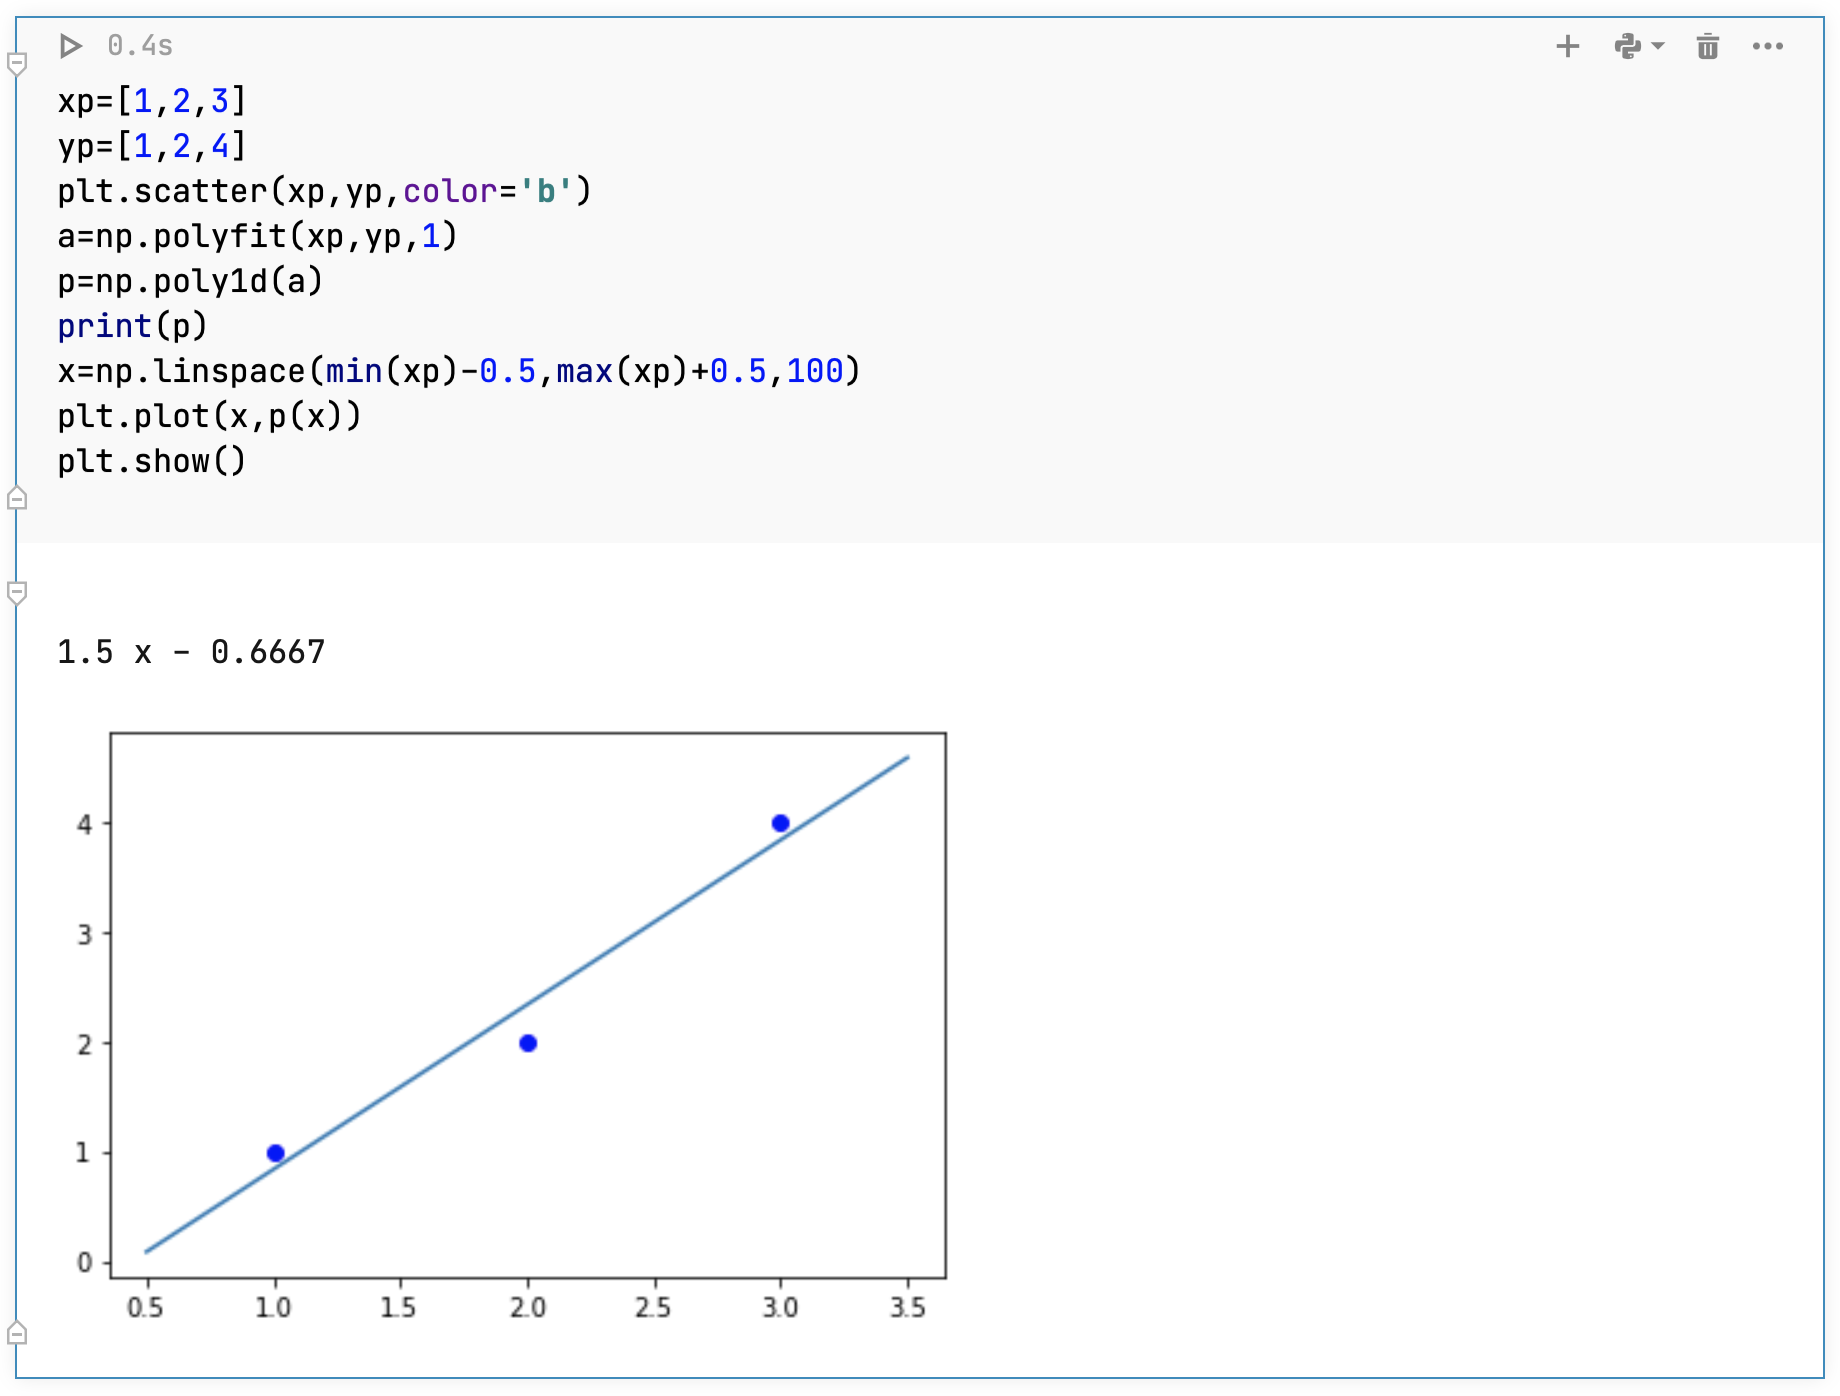
\includegraphics[width=10cm]{images/approximationRegression00.png}
\end{center}
\end{frame}
%\huge{Intégration numérique}

\begin{frame}
 \frametitle{Intégration numérique}
 Il s'agit d'approcher 
 \[ I =\int_a^b f(x) dx\]
dans le cas où on ne connaît pas une primitive de $f$.
Formule de quadrature
\[\myredbox{ \int_0^1 f(x) dx =\sum_{i=0}^{m-1}\omega_i f(\xi_i)}\]
Méthode de Newton Cotes . Les coefficient de quadrature $\omega_i$ sont calculer à l'aide d'une interpolation polynômiale de $f$ aux points 
\[\left\{\begin{array}{l}
\xi_k=\frac{k}{m-1}\mbox{ pour }i=0,\cdots, m-1\mbox{ si }m\neq 1\\
\xi=\frac{1}{2}\mbox{ si }m = 1
\end{array}\right.
\]
\end{frame}

\begin{frame}
Interpolation de Lagrange:
\[ f(x) \simeq \sum_{k=0}^{m-1}f(\xi_k)L_k(x)\]
où le polynôme $L_k(x)$ vérifie  $L_k(x_j)=\delta_{kj}$ et défini par
 \[L_k(x)=\prod_{i=0, i\neq k}^{m-1}\frac{x-x_i}{x_k-x_i}\]
d'où l'approximation
\[ \int_0^1 f(x)dx \simeq \int_0^1 \sum_{k=0}^{m-1}f(\xi_k) L_k(x)dx = \sum_{k=0}^{m-1}f(\xi_k)\underbrace{\int_0^1 L_k(x)dx}_{\omega_k}\]


 


\end{frame}

\begin{frame}
 \frametitle{ \fbox{$m=1$} }
 On a $\xi_0=\frac 12$ 
 
 D'autre part $L_0(x)=1$ donc \[\omega_0=\int_0^1 1 dx=1\]
  donc
\[\boxed{\int_0^1 f(x)dx \simeq f\left(\frac 12\right) }\]

\end{frame}

\begin{frame}
 \frametitle{ \fbox{$m=2$} }
 
 $\xi_0=0$, $\xi_1=1$ et

\begin{center}
  	\begin{tabular}{cc}
 \begin{tikzpicture}[scale=2]
\draw  [very thin, gray] [->]  (-0.2,0) -- (1.2,0); 
\draw  [very thin, gray] [->] (0,-0.2) -- (0,1.2);
\draw  [dashed] (0,0) -- (0,1);
\node [blue] at (0,0) {$\bullet$};
\node [blue] at (1,0) {$\bullet$};
\node at (0.5,-0.5) {$\scriptstyle  L_0(x)=1-x$};
\draw [orange,domain=0:1] plot(\x,1-\x);

\end{tikzpicture} 
 &
   \begin{tikzpicture}[scale=2]
\draw  [very thin, gray] [->]  (-0.2,0) -- (1.2,0); 
\draw  [very thin, gray] [->] (0,-0.2) -- (0,1.2);
\draw  [dashed] (1,0) -- (1,1);
\node [blue] at (0,0) {$\bullet$};
\node [blue] at (1,0) {$\bullet$};
\node at (0.5,-0.5) {$\scriptstyle L_1(x)=x$};
\draw [orange,domain=0:1] plot(\x,\x);

\end{tikzpicture} 
\end{tabular}
  	\end{center}

d'où 
\[\omega_0=\int_0^1 \left(1-x\right) dx=\frac 12\mbox{ et }\omega_1=\int_0^1 x\, dx=\frac 12\]
d'où
\[\boxed{\int_0^1 f(x)dx \simeq \frac{f\left(0 \right) + f\left(1 \right)}2}\]


\end{frame}

\begin{frame}
 \frametitle{ \fbox{$m=3$} } 
 
 $\xi_0=0$, $\xi_1=\frac 12$, $\xi_2=1$ et 

\begin{center}
  	\begin{tabular}{ccc}
 \begin{tikzpicture}[scale=2]
\draw  [very thin, gray] [->]  (-0.2,0) -- (1.2,0); 
\draw  [very thin, gray] [->] (0,-0.2) -- (0,1.2);
\draw  [dashed] (0,0) -- (0,1);
\node [blue] at (0,0) {$\bullet$};
\node [blue] at (0.5,0) {$\bullet$};
\node [blue] at (1,0) {$\bullet$};
\node at (0.5,-0.5) {$\scriptstyle L_0(x)=(2x-1)(x-1)$};
\draw [orange,domain=0:1] plot(\x,{(2*\x-1)*(\x-1)});

\end{tikzpicture} 
  &
  \begin{tikzpicture}[scale=2]
\draw  [very thin, gray] [->]  (-0.2,0) -- (1.2,0); 
\draw  [very thin, gray] [->] (0,-0.2) -- (0,1.2);
\node [blue] at (0,0) {$\bullet$};
\node [blue] at (0.5,0) {$\bullet$};
\node [blue] at (1,0) {$\bullet$};
\node at (0.5,-0.5) {$\scriptstyle L_1(x)=4x(1-x)$};
\draw [orange,domain=0:1] plot(\x,{4*\x*(1-\x)});

\end{tikzpicture} 
  &
  \begin{tikzpicture}[scale=2]
\draw  [very thin, gray] [->]  (-0.2,0) -- (1.2,0); 
\draw  [very thin, gray] [->] (0,-0.2) -- (0,1.2);
\draw  [dashed] (1,0) -- (1,1);
\node [blue] at (0,0) {$\bullet$};
\node [blue] at (0.5,0) {$\bullet$};
\node [blue] at (1,0) {$\bullet$};
\node at (0.5,-0.5) {$\scriptstyle L_2(x)=x(2x-1)$};
\draw [orange,domain=0:1] plot(\x,{\x*(2*\x-1)});

\end{tikzpicture} 
\end{tabular}
  	\end{center}

  donc \[\omega_0=\omega_1=\frac 16 \mbox{ et }\omega_2=\frac 23\]
d'où
\[\boxed{\int_0^1 f(x)dx \simeq \frac 16 \left(f\left(0 \right) +4\, f\left(\frac 12\right)+ f\left(1 \right)\right)}\]

\end{frame}

\begin{frame}
 \frametitle{Newton-Cotes sur $\left[a,b\right]$}
 On fait le changement de variable $x=a+\xi (b-a)$
 \[\begin{array}{ccl}
 \displaystyle \int_a^b f(x)dx &=& (b-a)\,\displaystyle \int_0^1 f(a+\xi (b-a))d\xi\\
                 &=&(b-a)\,\displaystyle{\sum_{k=0}^{m-1}\omega_k f(a+\xi_k (b-a))}
 \end{array}
 \]
\begin{itemize}
\item $m=1$ $\boxed{\int_a^b f(x)dx \simeq (b-a)\, f\left(\frac {a+b}2\right)}$
\item $m=2$ $\boxed{\int_a^b f(x)dx \simeq \frac{b-a}2\, \left(f\left(a\right)+f\left(b\right)\right)}$
\item $m=3$ $\boxed{\int_a^b f(x)dx \simeq \frac{b-a}6 \left(f\left(a \right) +4\, f\left(\frac{a+b}2\right)+ f\left(b \right)\right)}$
\end{itemize}

\end{frame}

\begin{frame}
 \frametitle{Etude de l'erreur}
\fbox{$m=1$} \\ Formule de Taylor Lagrange
\begin{center}
$\left|f(x)-f(\frac {a+b}2)+(x-\frac {a+b}2)f'(\frac {a+b}2)\right|\leq \frac{\left(x-\frac {a+b}2\right)^2}2\|f''\|$ 
\end{center}

d'où
\[\begin{array}{ccl}
\left|\int_a^bf(x)dx-(b-a)f(\frac {a+b}2)\right|&\leq &\frac 12 \int_a^b\left(x-\frac {a+b}2\right)^2dx \|f''\|\\
&\leq &\frac 12 \frac{(b-a)^3}{12}\|f''\|
\end{array}\]
D'où la majoration de l'erreur
\[\myredbox{|e|\leq \frac{(b-a)^3}{24}\|f''\|}\]




\end{frame}

\begin{frame}
 \frametitle{Etude de l'erreur}
\fbox{$m=2$} \\ D'après le théorème d'interpolation
\[f(x)-P(x) = \frac 12 (x-a)(x-b)f''(\xi)\]
d'où

\[\left|\int_a^bf(x)dx-\frac{b-a}6 \left(f\left(a \right) +4\, f\left(\frac{a+b}2\right)+ f\left(b \right)\right)\right|\]
\[\leq \frac 12\int_a^b\left| (x-a)(x-b)\right| \|f''\|\de x\]

D'où la majoration de l'erreur
\[\myredbox{|e|\leq \frac{(b-a)^3}{12}\|f''\|}\]




\end{frame}

\begin{frame}
 \frametitle{Etude de l'erreur}
\fbox{$m=3$} On admet la majoration de l'erreur
\[\myredbox{|e|\leq \frac{(b-a)^5}{2880}\|f^{(4)}\|}\]

En général,
\[f(x)-P(x)=\frac {L(x)}{m!}f^{(m)}(\xi)\]
d'où
\[|e|\leq \frac 1{m!}\left(\int_a^b\left|L(x)\right|dx \right)\|f^{(m)}\|\]
\end{frame}

\begin{frame}
 \frametitle{Méthode de rectangle}
\begin{center}
 \begin{tikzpicture}[domain=0:5]
  \draw[->] (-1.1,0) -- (6.1,0)  node[right] {$\scriptstyle x$};
  \draw[->] (-1,-0.1) -- (-1,2) node[above] {$\scriptstyle y$};
  \draw[dotted] (0,0) -- ++(0,0.707);
  \path[fill=black]  (0,0) circle (.4mm) [fill=gray] node[below] {$\scriptstyle a=x_0$};
 \path[fill=black]  (0,0) circle (.4mm) [fill=gray];
 \path[fill=black]  (1,0) circle (.4mm) [fill=gray];
 \path[fill=black]  (2,0) circle (.4mm) [fill=gray] node[below] {$\scriptstyle x_{i}$};
  
  \draw[orange,dotted] (2,0) -- ++(0,1.73);
  \draw[orange] (2,1.73) -- ++(1,0) node[right] {$\scriptstyle q_{i}$};
   \draw[orange,dotted] (3,0) -- ++(0,1.73);
    
 \path[fill=black]  (3,0) circle (.4mm) [fill=gray]node[below] {$\scriptstyle x_{i+1}$};
   \draw  (4.5,0.5) node {$\scriptstyle h$};
   \draw[<->] (4,0.2) -- ++(1,0) ;
   \path[fill=black]  (4,0) circle (.4mm) [fill=gray];
    \path[fill=black]  (5,0) circle (.4mm) [fill=gray] node[below] {$\scriptstyle b=x_n$};
   \draw [domain=0:5][line width=0.5] plot(\x,{sqrt(\x+0.5)});
 \draw[dotted] (5,0) -- ++(0,2.345);
\end{tikzpicture}
 \end{center}
 Subdivision: $x_i=a+i h$ avec $h=\frac{b-a}n$
 \[\int_{x_i}^{x_{i+1}}f(x)\de x=(x_{i+1}-x_i) f\left(\frac{x_i+x_{i+1}}{2}\right)=h \cdot f\left(x_{i+\frac 12}\right)\] 
\[\int_a^bf(x)\de x= \sum_{i=0}^{n-1}\int_{x_i}^{x_{i+1}}f(x)\de x=
h \sum_{i=0}^{n-1} f\left(x_{i+\frac 12}\right)\] 
 \[\myredbox{\int_a^bf(x)\de x= h \sum_{i=0}^{n-1} f\left(a+(i+\frac 12)h\right)}\] 
\end{frame}
%%%%%%%%%%%%%%%%%%%%%%%%%%%
\begin{frame}
 \frametitle{Exemple: $\displaystyle \int_0^1\frac{4}{x^2+1}\de x$}
%\begin{tabular}{cc}
\begin{tikzpicture}[scale=0.5]
\draw  [very thin, gray] [->]  (-1.2,0) -- (3.2,0); 
\draw  [very thin, gray] [->] (0,-1) -- (0,4.5);

\fill[color=gray!20]
(0,0) -- (0,1)
-- plot [domain=0:1] (\x,4/(\x*\x+1)
-- (1,0) -- cycle;
\draw [domain=-0.8:3,line width=0.5] plot(\x,4/(\x*\x+1)  ;
\end{tikzpicture} 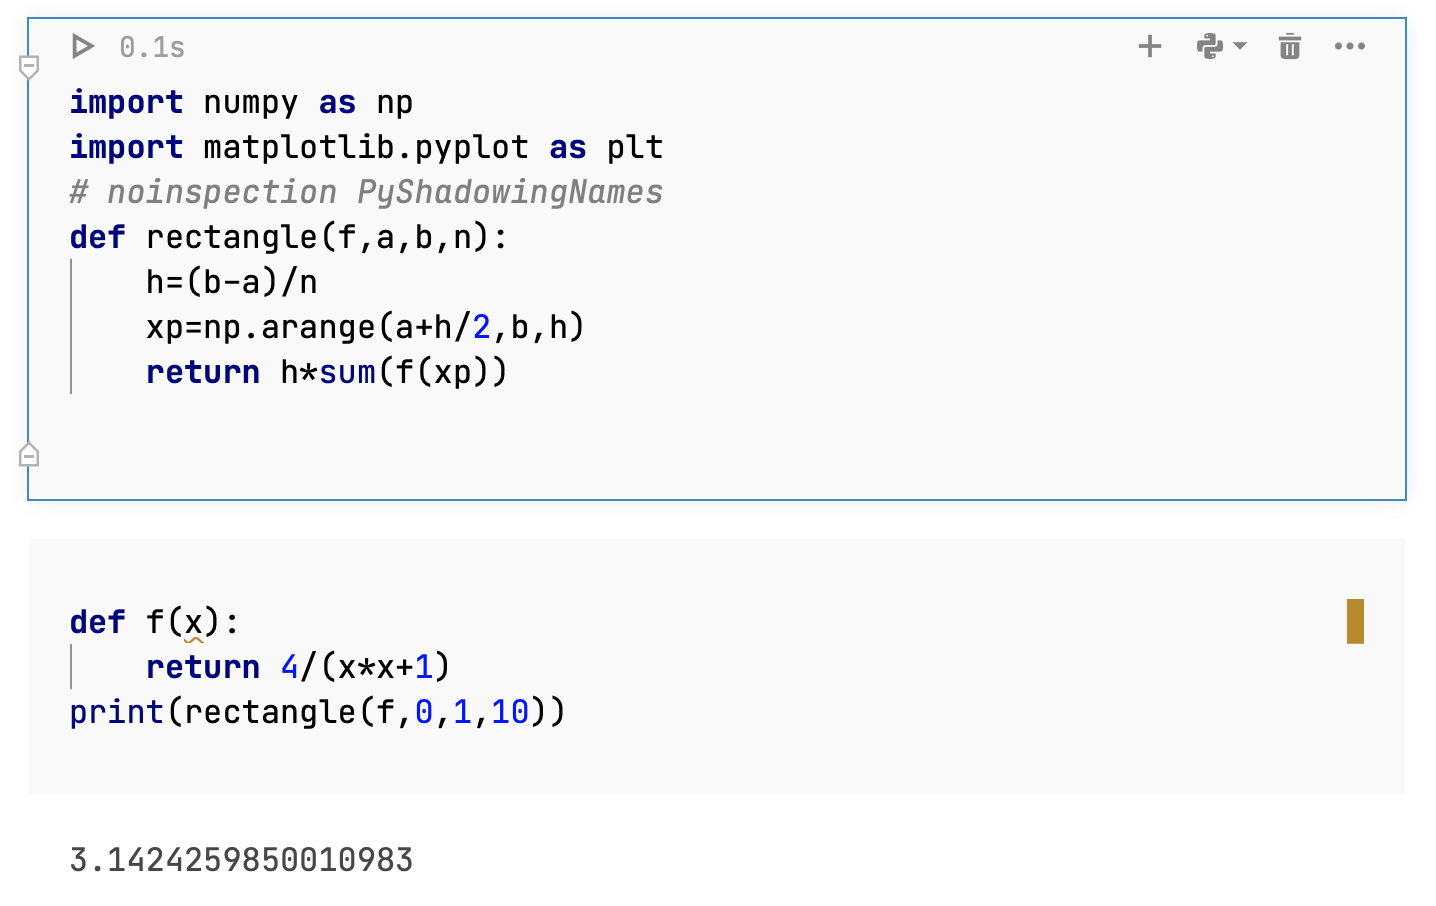
\includegraphics[width=8cm]{images/methodeDeRectangle00.png}
%\end{tabular}
 

\end{frame}
%%%%%%%%%%%%%%%%%%%%%%%%%%
\begin{frame}
 \frametitle{Erreur de la méthode de rectangle}
 On a 
 \[\left|\int_a^bf(x)dx-(b-a)f(\frac {a+b}2)\right|\leq \frac 12 \frac{(b-a)^3}{12}\|f''\|\]
 \[ \left|\int_{x_i}^{x_{i+1}}f(x)dx-h \cdot f(a+(i+\frac 12)h) \right|\leq  \frac{h^3}{24}\|f''\|\]
  \[ \sum_{i=0}^{n-1}  \left|\int_{x_i}^{x_{i+1}}f(x)dx-h \cdot f(a+(i+\frac 12)h) \right|\leq  \sum_{i=0}^{n-1}  \frac{h^3}{24}\|f''\|\]
  \[ \left| \sum_{i=0}^{n-1}  \left(  \int_{x_i}^{x_{i+1}}f(x)dx-h \cdot f(a+(i+\frac 12)h)\right) \right|\leq  \sum_{i=0}^{n-1}  \frac{h^3}{24}\|f''\|\]
  \[ \myredbox{\left| \int_a^bf(x)\de x -h  \sum_{i=0}^{n-1}  f(a+(i+\frac 12)h) \right| \leq   \frac{(b-a)^3}{24n^2}\|f''\|} \]
 \end{frame}
%%%%%%%%%%%%%%%%%%%%%%%%%%%
\begin{frame}
 \frametitle{Erreur: $\displaystyle E=\left|\pi - \int_0^1\frac{4}{x^2+1}\de x \right|$}
\begin{center}
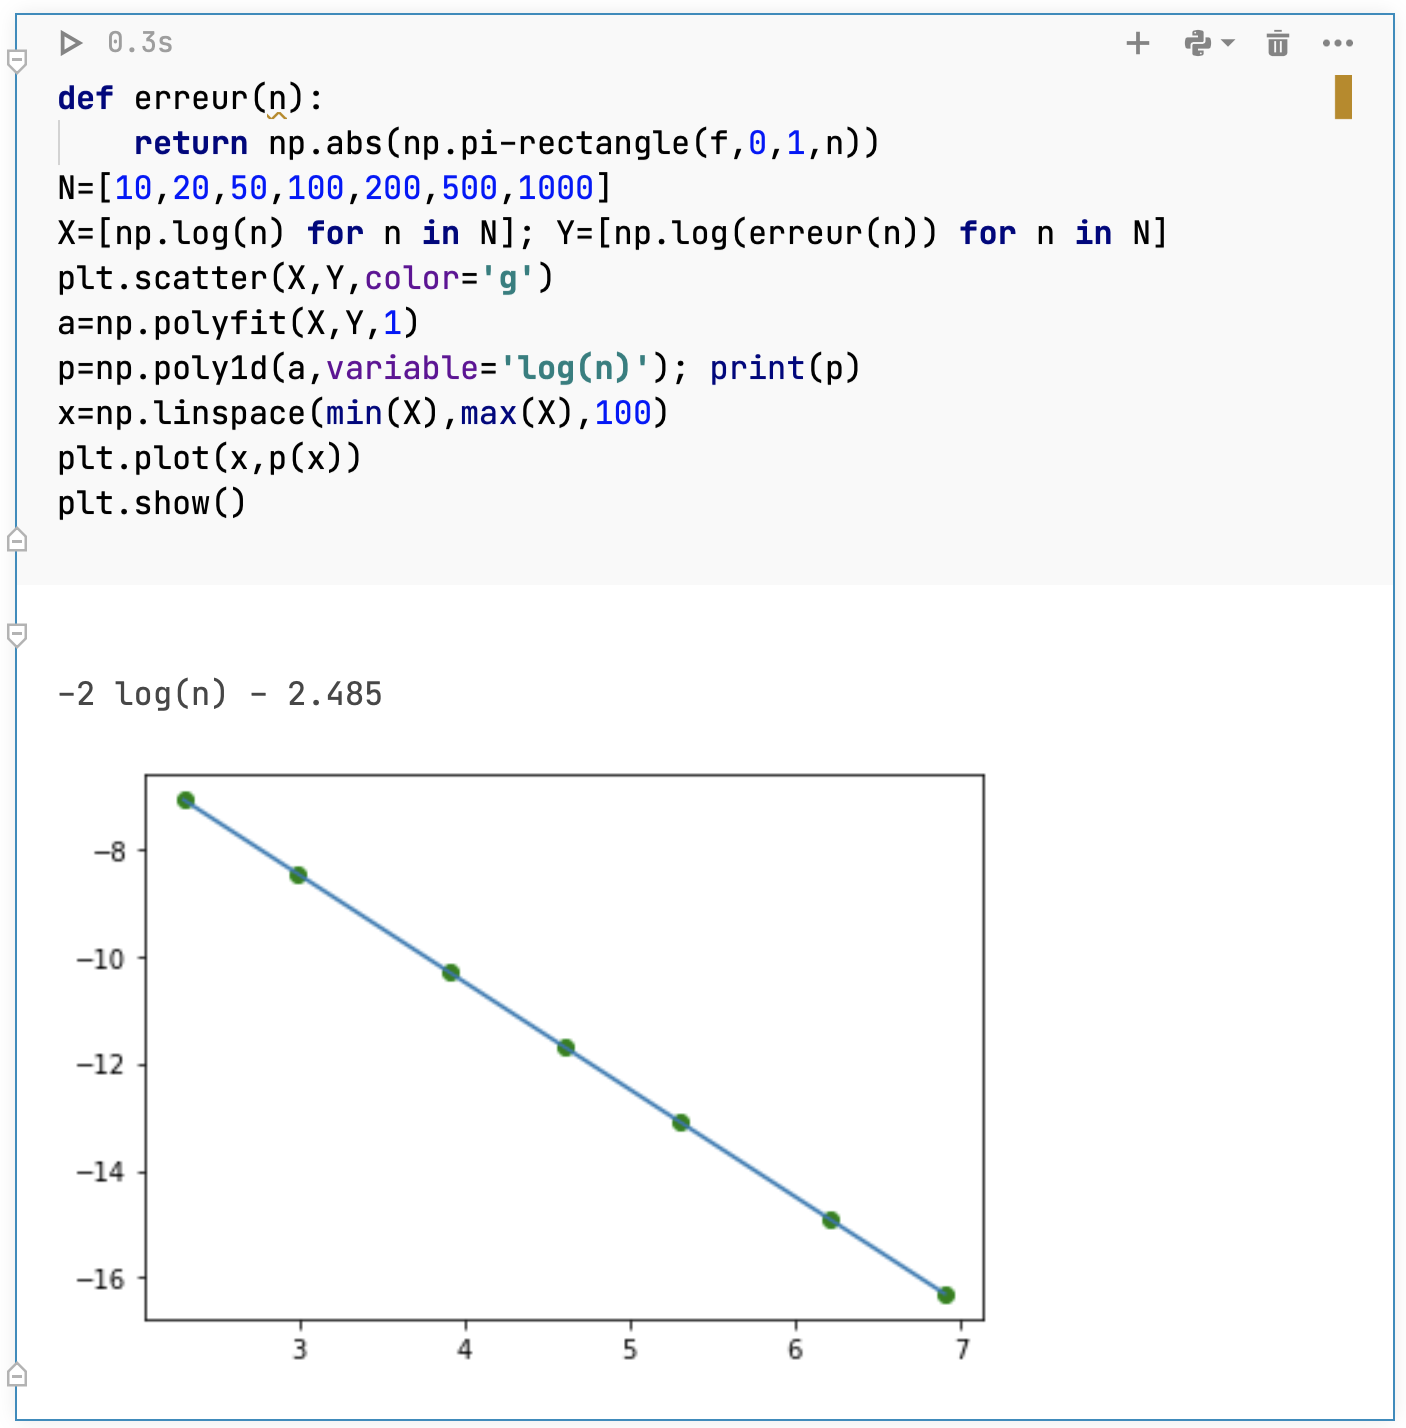
\includegraphics[width=7.5cm]{images/methodeDeRectangle01.png}
\end{center}
 

\end{frame}
%%%%%%%%%%%%%%%%%%%%%%%%%%
\begin{frame}
 \frametitle{Méthode de trapèze}
%\begin{center}
% \begin{tikzpicture}[domain=0:5]
%  \draw[->] (-1.1,0) -- (6.1,0)  node[right] {$\scriptstyle x$};
%  \draw[->] (-1,-0.1) -- (-1,2) node[above] {$\scriptstyle y$};
%  \draw[dotted] (0,0) -- ++(0,0.707);
%  \path[fill=black]  (0,0) circle (.4mm) [fill=gray] node[below] {$\scriptstyle a=x_0$};
% \path[fill=black]  (0,0) circle (.4mm) [fill=gray];
% \path[fill=black]  (1,0) circle (.4mm) [fill=gray];
% \path[fill=black]  (2,0) circle (.4mm) [fill=gray] node[below] {$\scriptstyle x_{i}$};
%  
%  \draw[orange,dotted] (2,0) -- ++(0,1.73);
%  \draw[orange] (2,1.73) -- ++(1,0) node[right] {$\scriptstyle q_{i}$};
%   \draw[orange,dotted] (3,0) -- ++(0,1.73);
%    
% \path[fill=black]  (3,0) circle (.4mm) [fill=gray]node[below] {$\scriptstyle x_{i+1}$};
%   \draw  (4.5,0.5) node {$\scriptstyle h$};
%   \draw[<->] (4,0.2) -- ++(1,0) ;
%   \path[fill=black]  (4,0) circle (.4mm) [fill=gray];
%    \path[fill=black]  (5,0) circle (.4mm) [fill=gray] node[below] {$\scriptstyle b=x_n$};
%   \draw [domain=0:5][line width=0.5] plot(\x,{sqrt(\x+0.5)});
% \draw[dotted] (5,0) -- ++(0,2.345);
%\end{tikzpicture}
% \end{center}

 \[\int_{x_i}^{x_{i+1}}f(x)\de x=(x_{i+1}-x_i) \frac{f(x_i)+f(x_{i+1})}{2}\] 
\[\int_a^bf(x)\de x= \sum_{i=0}^{n-1}\int_{x_i}^{x_{i+1}}f(x)\de x=
h \sum_{i=0}^{n-1}\frac{f(x_i)+f(x_{i+1})}{2}\] 
 \[\myredbox{\int_a^bf(x)\de x= h \left[\frac{f(a)+f(b)}{2}  + \sum_{i=1}^{n-1} f(x_i)\right]}\] 
 Erreur de la méthode de trapèze
 \[ \myredbox{\left| \int_a^bf(x)\de x -h \left(\frac{f(a)+f(b)}{2}  + \sum_{i=1}^{n-1} f(x_i)\right)\right| \leq   \frac{(b-a)^3}{12n^2}\|f''\|} \]
\end{frame}
%%%%%%%%%%%%%%%%%%%%%%%%%%%
\begin{frame}
 \frametitle{Exemple: $\displaystyle \int_0^1\frac{4}{x^2+1}\de x$}
%\begin{tabular}{cc}
\begin{tikzpicture}[scale=0.5]
\draw  [very thin, gray] [->]  (-1.2,0) -- (3.2,0); 
\draw  [very thin, gray] [->] (0,-1) -- (0,4.5);

\fill[color=gray!20]
(0,0) -- (0,1)
-- plot [domain=0:1] (\x,{4/(\x*\x+1)})
-- (1,0) -- cycle;
\draw [domain=-0.8:3,line width=0.5] plot(\x,{4/(\x*\x+1)})  ;
\end{tikzpicture} 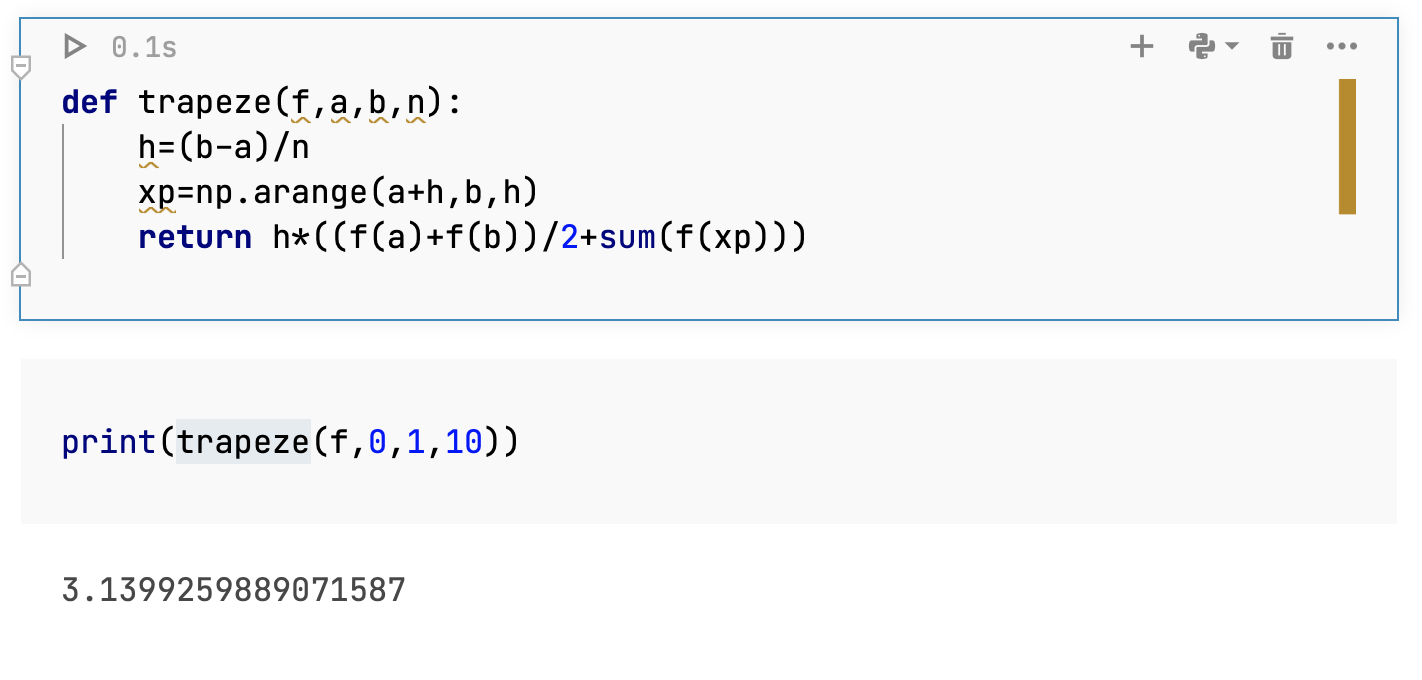
\includegraphics[width=8cm]{images/methodeDeTrapeze00.png}
%\end{tabular}
 

\end{frame}
%%%%%%%%%%%%%%%%%%%%%%%%%%
%%%%%%%%%%%%%%%%%%%%%%%%%%%
\begin{frame}
 \frametitle{Erreur: $\displaystyle E=\left|\pi - \int_0^1\frac{4}{x^2+1}\de x \right|$}
\begin{center}
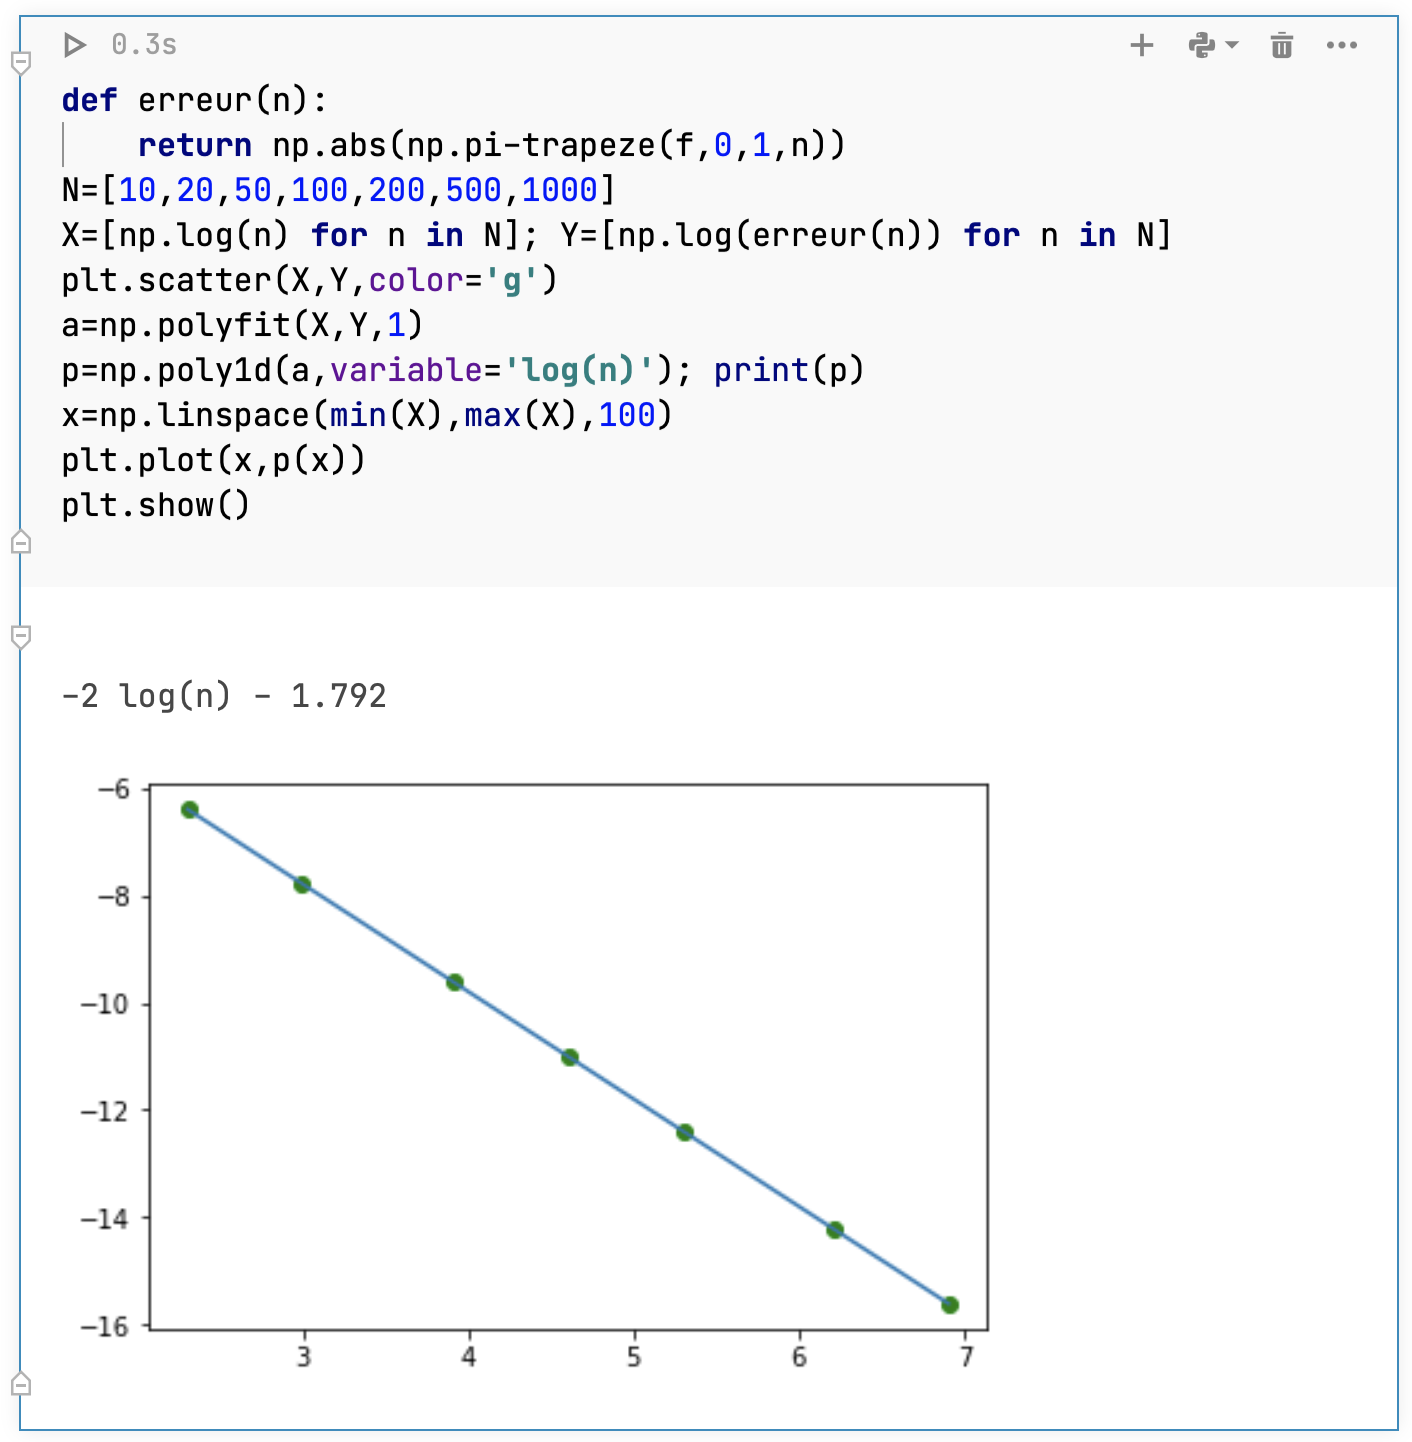
\includegraphics[width=7.5cm]{images/methodeDeTrapeze01.png}
\end{center}
 

\end{frame}
%%%%%%%%%%%%%%%%%%%%%%%%%%
\begin{frame}
 \frametitle{Méthode de Simpson}
  \[\int_{x_i}^{x_{i+1}}f(x)\de x=\frac{(x_{i+1}-x_i)}{6} \left[f(x_i)+4\cdot f\left(\frac{x_i+x_{i+1}}{2}\right) +f(x_{i+1})\right]\] 
 \[\myredbox{\int_a^bf(x)\de x= \frac{b-a}{6n}  \sum_{i=0}^{n-1} \left[f(x_i)+4\cdot f\left(\frac{x_i+x_{i+1}}{2}\right) +f(x_{i+1})\right] }\] 
 Erreur de la méthode de Simpson
 \[ \myredbox{\left| \int_a^bf(x)\de x -\frac{b-a}{6n}  \sum_{i=0}^{n-1} \left[f(x_i)+4\cdot 
 f\left(x_{i+1/2}\right) +f(x_{i+1})\right] \right| \leq   \frac{(b-a)^5}{2880n^4}M_4} \]
 \end{frame}
%%%%%%%%%%%%%%%%%%%%%%%%%%%
\begin{frame}
 \frametitle{Exemple: $\displaystyle \int_0^\frac{\pi}{2}\cos x\de x$}
%\begin{tabular}{cc}
\begin{tikzpicture}[xscale=0.5]
\draw  [very thin, gray] [->]  (-0.8,0) -- (4,0); 
\draw  [very thin, gray] [->] (0,-1) -- (0,1.5);

\fill[color=gray!20]
(0,0) -- (0,1)-- plot [domain=0:1.57] (\x,{cos(\x*180/pi)}) -- cycle;
\draw [domain=-0.8:4,line width=0.5] plot(\x,{cos(\x*180/pi)});
\end{tikzpicture} 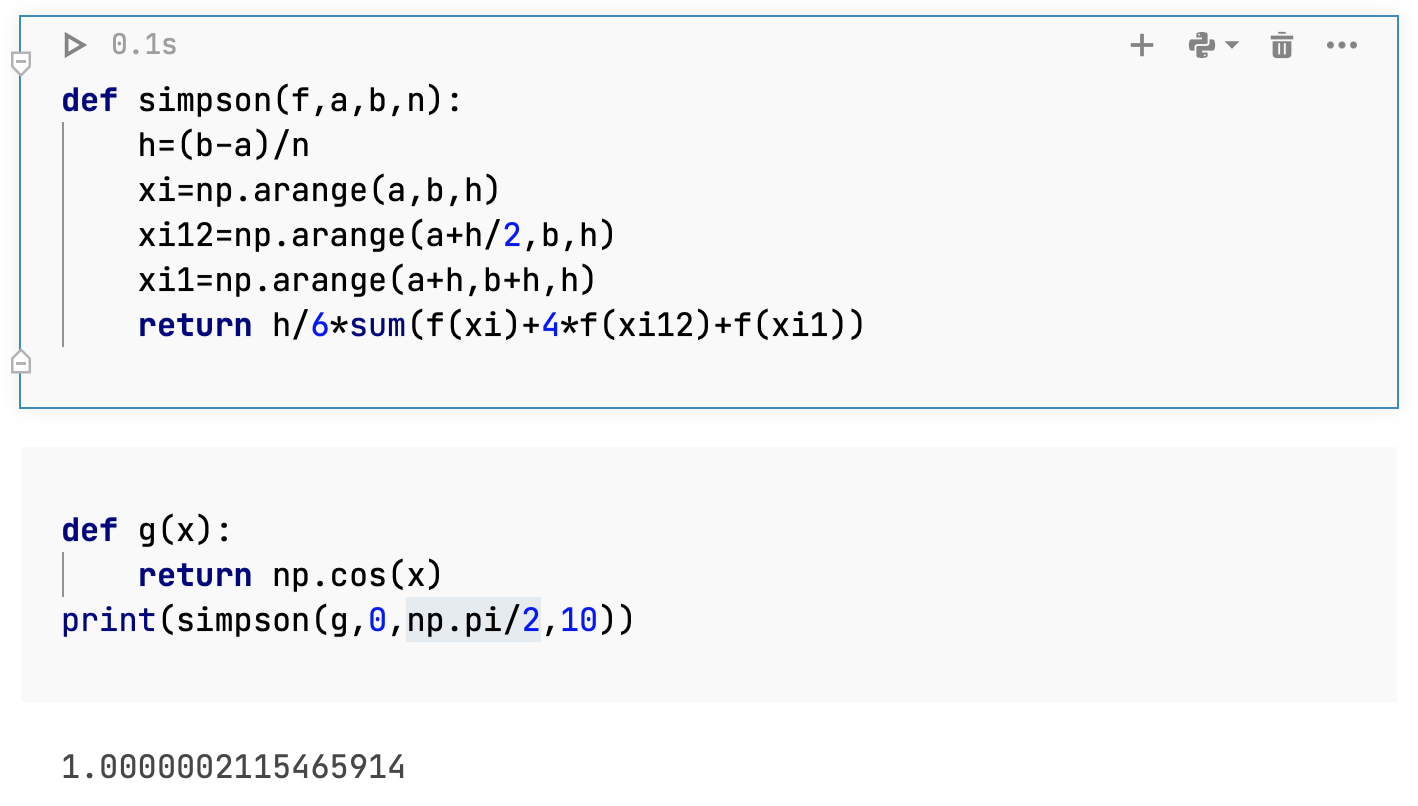
\includegraphics[width=8cm]{images/methodeDeSimpson00.png}
%\end{tabular}
 

\end{frame}
%%%%%%%%%%%%%%%%%%%%%%%%%%
%%%%%%%%%%%%%%%%%%%%%%%%%%%
\begin{frame}
 \frametitle{Erreur: $\displaystyle E=\left|1 - \int_0^\frac{\pi}{2}\cos x\de x \right|\sim\frac{C}{n^\alpha}$}
\begin{center}
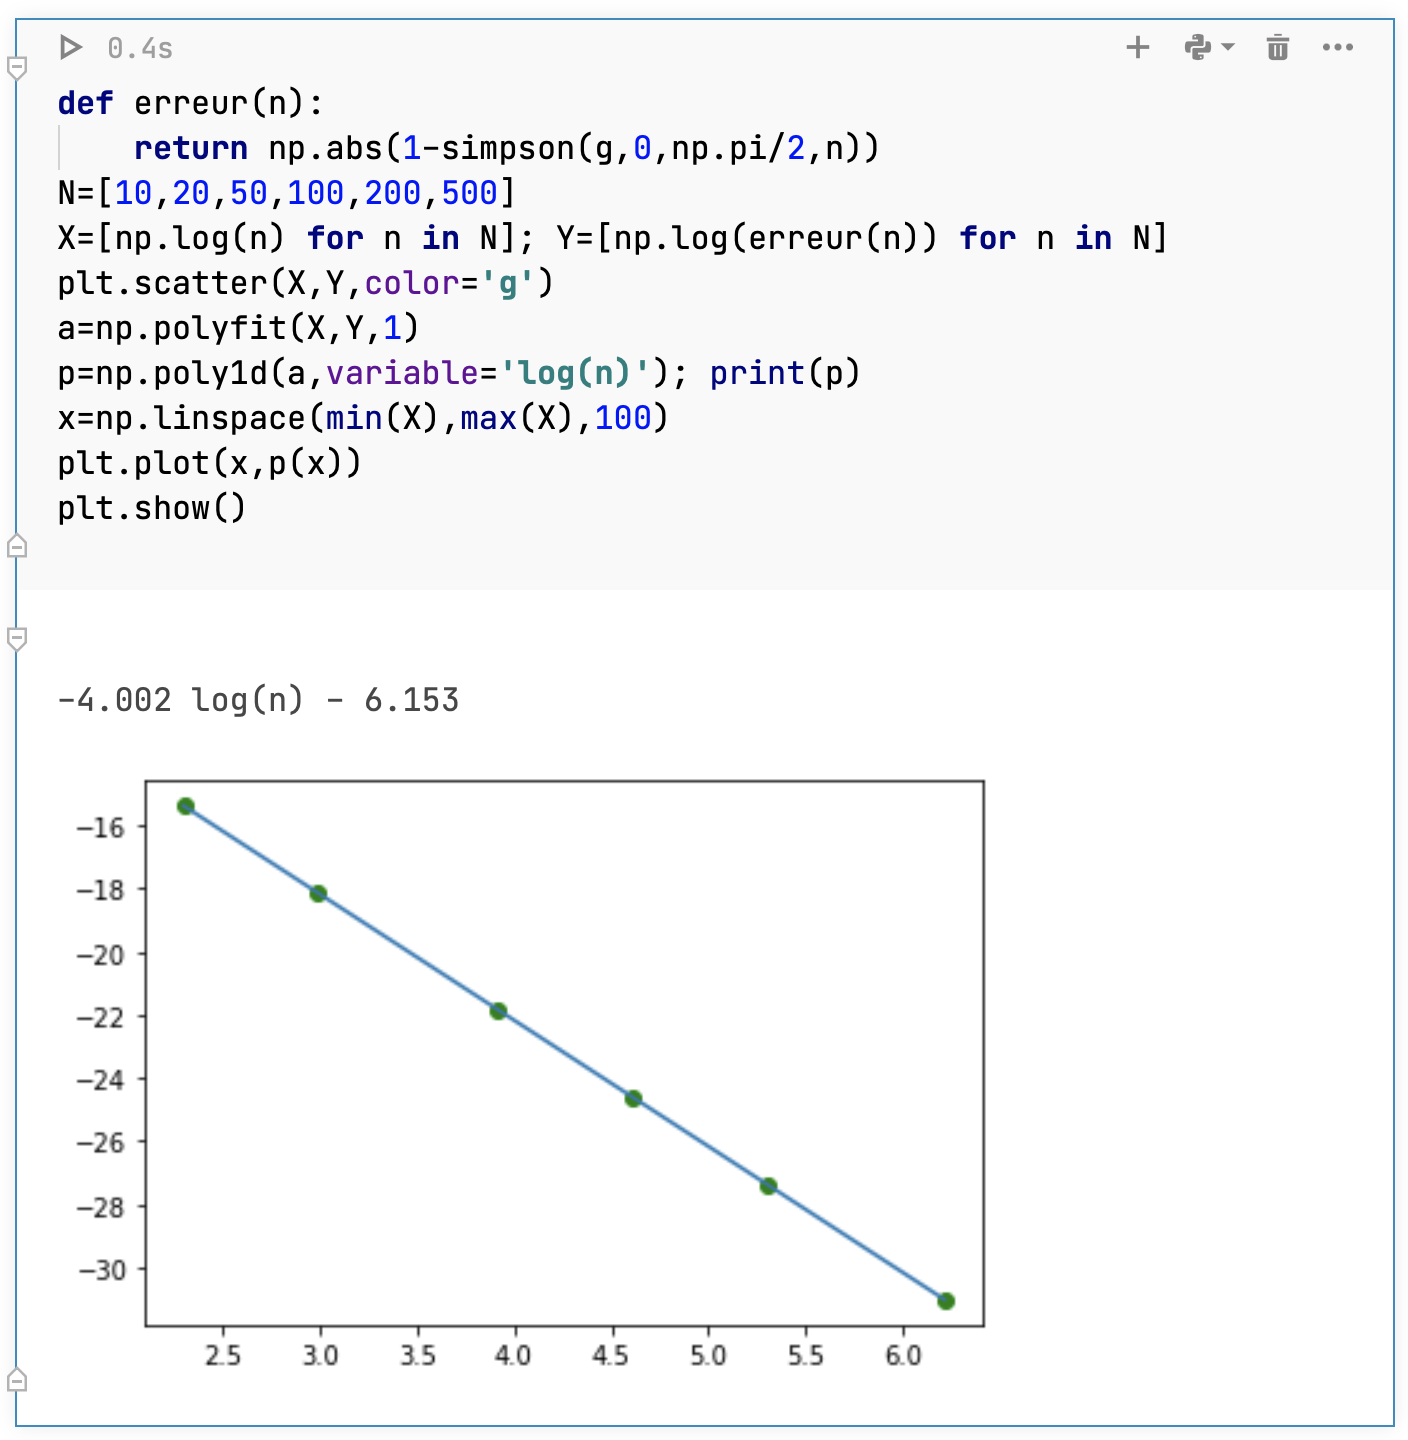
\includegraphics[width=7.5cm]{images/methodeDeSimpson01.png}
\end{center}
 

\end{frame}
%%%%%%%%%%%%%%%%%%%%%%%%%%

\begin{frame}
 \frametitle{Méthode de Gauss}
 La méthode de quadrature de Gauss,  consiste à remplacer le calcul de l'intégrale par une somme pondérée prise en $n$ points du domaine d'intégration: 
 \[\myredbox{ \int_{-1}^1 f(x) dx \simeq \sum_{i=1}^{n}\omega_i f(\xi_i)}\]
  Elle est  exacte pour les polynômes de degré $2n-1$. 
  
 \begin{block}{Exercice}
 Pour $n=2$ Déterminer les poids $\omega_1$, $\omega_2$ et les points $\xi_1$ et $\xi_2$ de la formule de quadrature de Gauss
  \[ \int_{-1}^1 f(x) dx \simeq \omega_1 f(\xi_1)+\omega_2 f(\xi_2)\]
 \end{block}
 
  
 \end{frame}




\begin{frame}
 \frametitle{Méthode de Gauss}
 Si la formule est exacte pour les polynômes de degré au plus  $2n-1=3$, elle doit être donc  exacte pour $f(x)=1$,  $f(x)=x$, $f(x)=x^2$, $f(x)=x^3$.
  \[\begin{array}{l}
   \int_{-1}^1 1 dx = \omega_1 \times 1+\omega_2 \times 1 \Longrightarrow \omega_1 +\omega_2=2\\
    \int_{-1}^1 x dx = \omega_1 \times \xi_1+\omega_2 \times \xi_2 \Longrightarrow \omega_1\xi_1 +\omega_2\xi_2=0\\
     \int_{-1}^1 x^2 dx = \omega_1 \times \xi_1^2+\omega_2 \times \xi_2^2 \Longrightarrow \omega_1\xi_1^2 +\omega_2\xi_2^2=\frac 23\\
     \int_{-1}^1 x^3 dx = \omega_1 \times \xi_1^3+\omega_2 \times \xi_2^3 \Longrightarrow \omega_1\xi_1^3 +\omega_2\xi_2^3=0
\end{array}  \]
D'où le système non linéaire de 4 équations à 4 inconnues
\begin{tabular}{cc}
$\left\{\begin{array}{l}
    \omega_1 +\omega_2=2\\
    \omega_1\xi_1 +\omega_2\xi_2=0\\
      \omega_1\xi_1^2 +\omega_2\xi_2^2=\frac 23\\
      \omega_1\xi_1^3 +\omega_2\xi_2^3=0
\end{array} \right. $  &\begin{tabular}{c}
La deuxième et le troisième équations donnent:\\

$\left.\begin{array}{l}
    \omega_1\xi_1 =-\omega_2\xi_2\\
      \omega_1\xi_1^3 =-\omega_2\xi_2^3
\end{array} \right\}\Longrightarrow \xi_1^2 =\xi_2^2 $  \\
$\Longrightarrow \xi_1 =-\xi_2=\sqrt{\frac{1}{3}}$ et $\omega_1 =\omega_2=1$
\end{tabular}
\end{tabular}

 \end{frame}
 
 \begin{frame}
 \frametitle{Exercice: Méthode de Gauss}
D'où la formule de quadrature
\[ \myredbox{ \int_{-1}^1 f(x) dx \simeq f(-\frac 1{\sqrt 3})+ f(\frac 1{\sqrt 3})}\]
 Par changement de variable $x=\frac{a+b}{2}+\xi \frac{b-a}{2}$, on a
 \[ \int_{a}^b f(x) dx \simeq \frac{b-a}2\left[f(\frac{a+b}{2}-\frac 1{\sqrt 3}\frac{b-a}{2} )+ f(\frac{a+b}{2}+\frac 1{\sqrt 3}\frac{b-a}{2} )\right]\]
  \[ \int_{x_i}^{x_{i+1}} f(x) dx \simeq\frac h2\left[ f(x_{i+1/2}-\frac h{2\sqrt 3} )+ f(x_{i+1/2}+\frac h{2\sqrt 3})\right]\]
   \[ \myredbox{ \int_{a}^b f(x) dx  \simeq\frac h2\sum_{i=0}^{N-1}\left[ f(x_{i+1/2}-\frac h{2\sqrt 3} )+ f(x_{i+1/2}+\frac h{2\sqrt 3})\right]}\]
 \end{frame}

 
\begin{frame}
 \frametitle{Théorème:  Méthode de Gauss}
Il existe un unique choix des $(\omega_i)$ et $(\xi_i)$ tels que la méthode
  \[\myredbox{  \int_{\alpha}^{\beta} f(x)w(x) dx \simeq \sum_{i=1}^{n}\omega_i f(\xi_i)}\]
soit d'ordre $N=2n-1$. Les points $(\xi_i)$  sont dans$]\alpha,\beta[$ et sont les racines du $n$-ième polynôme orthogonal pour le poids $w$.  
 \end{frame}
\begin{frame}
\frametitle{Polynômes orthogonaux}

Nous considérerons dans toute la suite un intervalle $I=(a,b)$ de $\mathbb{R}$
, borné ou non, et une fonction $\omega > 0$ sur $I$, appelée poids, qui vérifie pour tout $n\in\mathbb{N}$
\[\int_a^b|x|^n\omega(x)dx<\infty\]
Tout polynôme est donc intégrable pour la mesure de densité $\omega$ par rapport à la mesure de Lebesgue sur $I$. Nous définissons sur l'espace vectoriel $E=\mathbb{R}[X]$ le produit scalaire
\[\myredbox{(P,Q)=\int_a^b \omega(x) P(x) Q(x) dx}\]
\begin{theorem}
Il existe une suite de polynômes $\left(P_k\right)_k$ et une seule vérifiant :
\begin{itemize}
\item Pour tout $k$, le degré de $P_k$ est $k$ et $P_k$ est unique.
\item Pour tous $k \neq j$, $(P_j , P_k) = 0$ (ce qui implique que, pour tout $k$,
$\left(P_k\right)_k$ est une base de $E_k=\mathbb{R}_k[X]$ et que $P_k$ est orthogonal à $E_{k-1}$.
\end{itemize}
\end{theorem}
\end{frame}


\begin{frame}
Le procédé d'orthogonalisation de Schmidt permet alors de construire à partir de la base naturelle $(1,X,...,X^n)$ de $E_n$ une famille orthogonale de polynômes qu'on peut supposer unitaires.  Cette familles vérifie une relation de récurrence qui s'écrit:
\[\myredbox{P_n(x)=(x-\lambda_n)P_{n-1}(x)-\mu_n P_{n-2}(x)}\]
avec $\lambda_n=\frac{(xP_{n-1},P_{n-1})}{\|P_{n-1}\|^2}$ et $\mu_n=\frac{\|P_{n-1}\|^2}{\|P_{n-2}\|^2}$ 
En pratique, on commence la récurrence avec les deux polynômes 
\[P_{-1}(x)=0\mbox{ et } P_{0}(x)=1\]
\end{frame}


\begin{frame}
\frametitle{polynômes de Legendre}
Les polynômes de Legendre correspondent au cas particulier $a =-1$, $b=1$ et $\omega(x) = 1$.


La formule de Rodrigues permet un calcul direct de la famille orthogonale  de polynômes (non unitaires) de Legendre $(P_n)_n$ :
\[ \myredbox{P_n(x)=\frac 1{2^n n!}\frac{\mbox{d}^n}{\mbox{d}x^n}\left[(x^2-1)^n\right]}\]
 
La relation de récurrence s'écrit
\[\myredbox{n\,P_n(x)=(2n-1)x\,P_{n-1}(x)-(n-1) P_{n-2}(x)}\]
pour $n\geq 2$ où $P_0(x)=1$ et  $P_1(x)=x$. 

En appliquant la relation de récurrence, on trouve
\[P_2(x)=\frac 12\left(3x^2-1\right),\qquad P_3(x)=\frac 12\left(5x^3-3x\right),\qquad  \cdots \]

\end{frame}


\begin{frame}
\frametitle{Polynômes de Tchebychef}
\begin{theorem}
 Les polynômes $T_n(x)$, tels que $T_n(\cos\theta) = \cos n\theta$, sont orthogonaux relativement au poids $\omega(x)=\frac 1{\sqrt{1-x^2}}$ sur $[-1,1]$
\end{theorem}
En effet par le changement de variables $x = \cos\theta$, avec $\theta \in [0, \pi]$:
\[\int_{-1}^1\frac 1{\sqrt{1-x^2}}T_n(x) T_m(x) \de x=\int_0^{\pi}\cos n\theta\cos m\theta \de \theta=0\quad\mbox{si }m\neq n\]
La relation de récurrence s'écrit
\[P_n(x)=2x\,P_{n-1}(x)- P_{n-2}(x)\]
pour $n\geq 2$ où $P_0(x)=1$ et  $P_1(x)=x$. 

En appliquant la relation de récurrence, on trouve
\[P_2(x)=2x^2-1,\qquad P_3(x)=4x^3-3x,\qquad  \cdots \]
\end{frame}


\begin{frame}
\begin{block}{Polynômes d'Hermite}
C'est le cas particulier $a =-\infty$, $b=\infty$ et $\omega(x) = \exp(-x^2)$.
\end{block}

\begin{block}{Polynômes de Laguerre}
C'est le cas particulier $a =0$, $b=\infty$ et $\omega(x) = \exp(-x)$.
\end{block}
\end{frame}

\begin{frame}
\begin{block}{Méthode de Gauss-Legendre}
\begin{itemize}
\item les points $\xi_k$ sont les racines du polynôme de Legendre $P_n$ :
\[
\myredbox{
\begin{array}{l}
P_{-1}(x)=0 \\
P_0(x)=1\\
n\,P_n(x)=(2n-1)x\,P_{n-1}(x)-(n-1) P_{n-2}(x)
\end{array}
}\]
\[P_0(x)=1, P_1(x)=x, P_2(x)=(3x^2-1)/2, \cdots\]
\item Les $n$ coefficients associés valent respectivement :
\[\myredbox{\forall k =1,\cdots n\quad \omega_k=\frac{2}{(1-\xi_k^2)P'_n(\xi_k)^2}}\]
\end{itemize}
\begin{center}
\begin{tabular}{c|c|c}
$n$ & $\omega_k$ & $\xi_k$\\ \hline
1 & 2 & 0 \\ \hline
2 & 1,1 & $-1/\sqrt 3$, $1/\sqrt 3$\\ \hline
3& 5/9, 8/9, 5/9 & $-\sqrt{3/5}$, 0, $\sqrt{3/5}$
\end{tabular}
\end{center}
\end{block}
\end{frame}
%%%%%%%%%%%%%%%%%%%%%%%%%%%%%%%%%%%%%%%%%%%%%%%%

\begin{frame}
\frametitle{Exemple: Formule de Gauss-Legendre pour $n=3$:}

\[ \int_0^1f(x)\de x = \frac 59f\left(-\sqrt{\frac 35}\right)+\frac 89 f(0)+\frac 59f\left(+\sqrt{\frac 35}\right)\]
\[ \int_a^bf(x)\de x = \frac{b-a}{2} \left[\frac 59f(\frac{a+b}2-\sqrt{\frac 35}\frac{b-a}2)+\frac 89 f(\frac{a+b}2)+\frac 59f(\frac{a+b}2+\sqrt{\frac 35}\frac{b-a}2)\right]\]
\[ \int_{x_{2i}}^{x_{2i+2}}f(x)\de x =\frac{h}{9} \left[5f(x_{2i+1}-\sqrt{\frac 35}h)+8f(x_{2i+1})+5f(x_{2i+1}+\sqrt{\frac 35}h)\right]\]
\[ \int_a^bf(x)\de x = \frac{h}{9} \sum_{i=0}^{N-1}\left[5f(x_{2i+1}-\sqrt{\frac 35}h)+8f(x_{2i+1})+5f(x_{2i+1}+\sqrt{\frac 35}h)\right]\]
où $h=\frac{b-a}{2N}$ et $x_i=a+ih$.
\end{frame}


%%%%%%%%%%%%%%%%%%%%%%%%%%%%%%%%%%%%%%%%%%%%%%%

\begin{frame}
\begin{block}{Méthode de Gauss-Tchebychev}
Polynômes de Tchebychev
\begin{center}
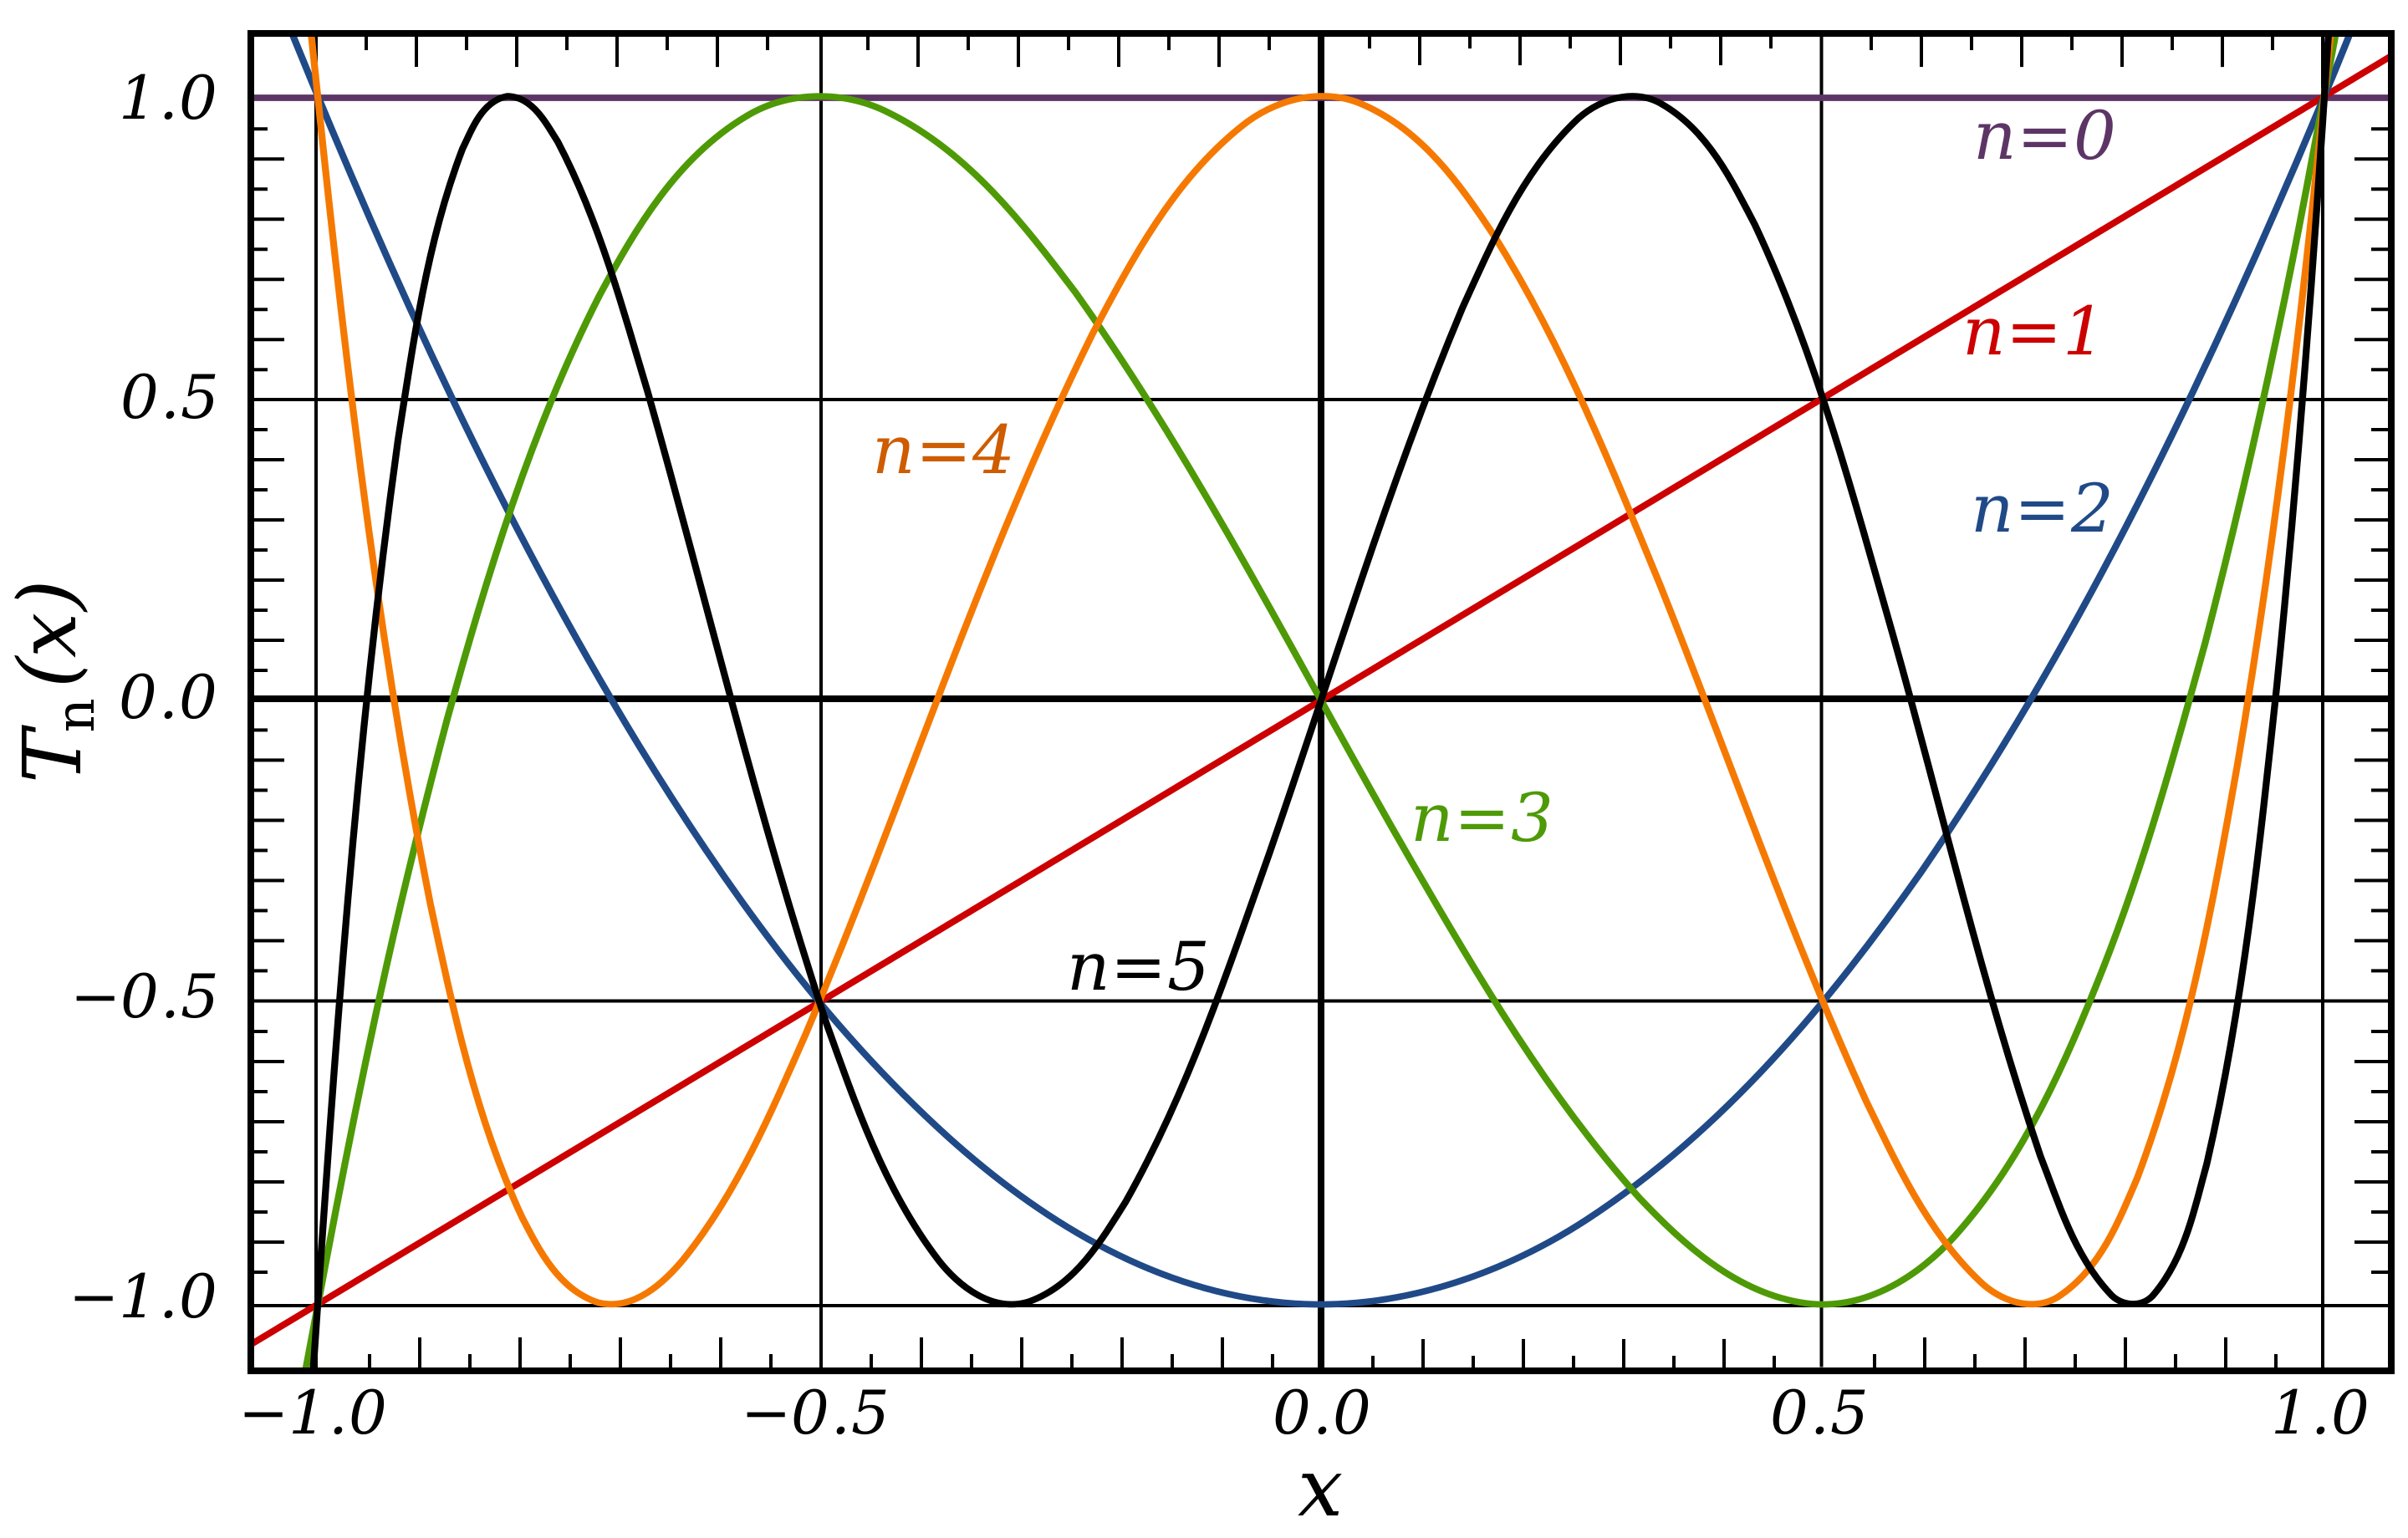
\includegraphics[width=5cm]{Chebyshev_Polynomials.png}
\end{center}
Pour $n$ points, les nœuds et les coefficients  sont
\[\myredbox{\forall k =1,\cdots n\quad  \xi_k = \cos \left(\frac{(2k-1)\pi}{2n}\right) \quad\mbox{ et }\quad \omega_k=\frac{\pi}{n} }\]

\end{block}
\end{frame}


\begin{frame}
\begin{block}{Méthode de Gauss-Tchebychev}

D'où
\[\myredbox{\int_{-1}^1\frac{f(x)}{\sqrt{1-x^2}}\de x =\frac{\pi}{n}\sum_{k=1}f( \cos \left(\frac{(2k-1)\pi}{2n}\right))}\]
Pour $n=2$
\[\int_{-1}^1\frac{f(x)}{\sqrt{1-x^2}}\de x =\frac{\pi}{2}\left( f( -\sqrt{2}/2)+f(\sqrt{2}/2)\right)\]
en particulier 
\[\int_{-1}^1\frac{x^2}{\sqrt{1-x^2}}\de x =\frac{\pi}{2}\]
\end{block}
\end{frame}

\begin{frame}
\begin{block}{Méthode de Gauss-Laguerre}
\begin{itemize}
\item les points $\xi_k$ sont les racines du polynôme de Laguerre $L_n$ :
\[
\myredbox{
\begin{array}{l}
L_{-1}(x)=0 \\
L_0(x)=1\\
n\,L_n(x)=(2n-1-x)\,L_{n-1}(x)-(n-1) L_{n-2}(x)
\end{array}
}\]
\[L_0(x)=1, L_1(x)=-x-1, L_2(x)=(x^2-4x+2)/2, \cdots\]

\begin{center}
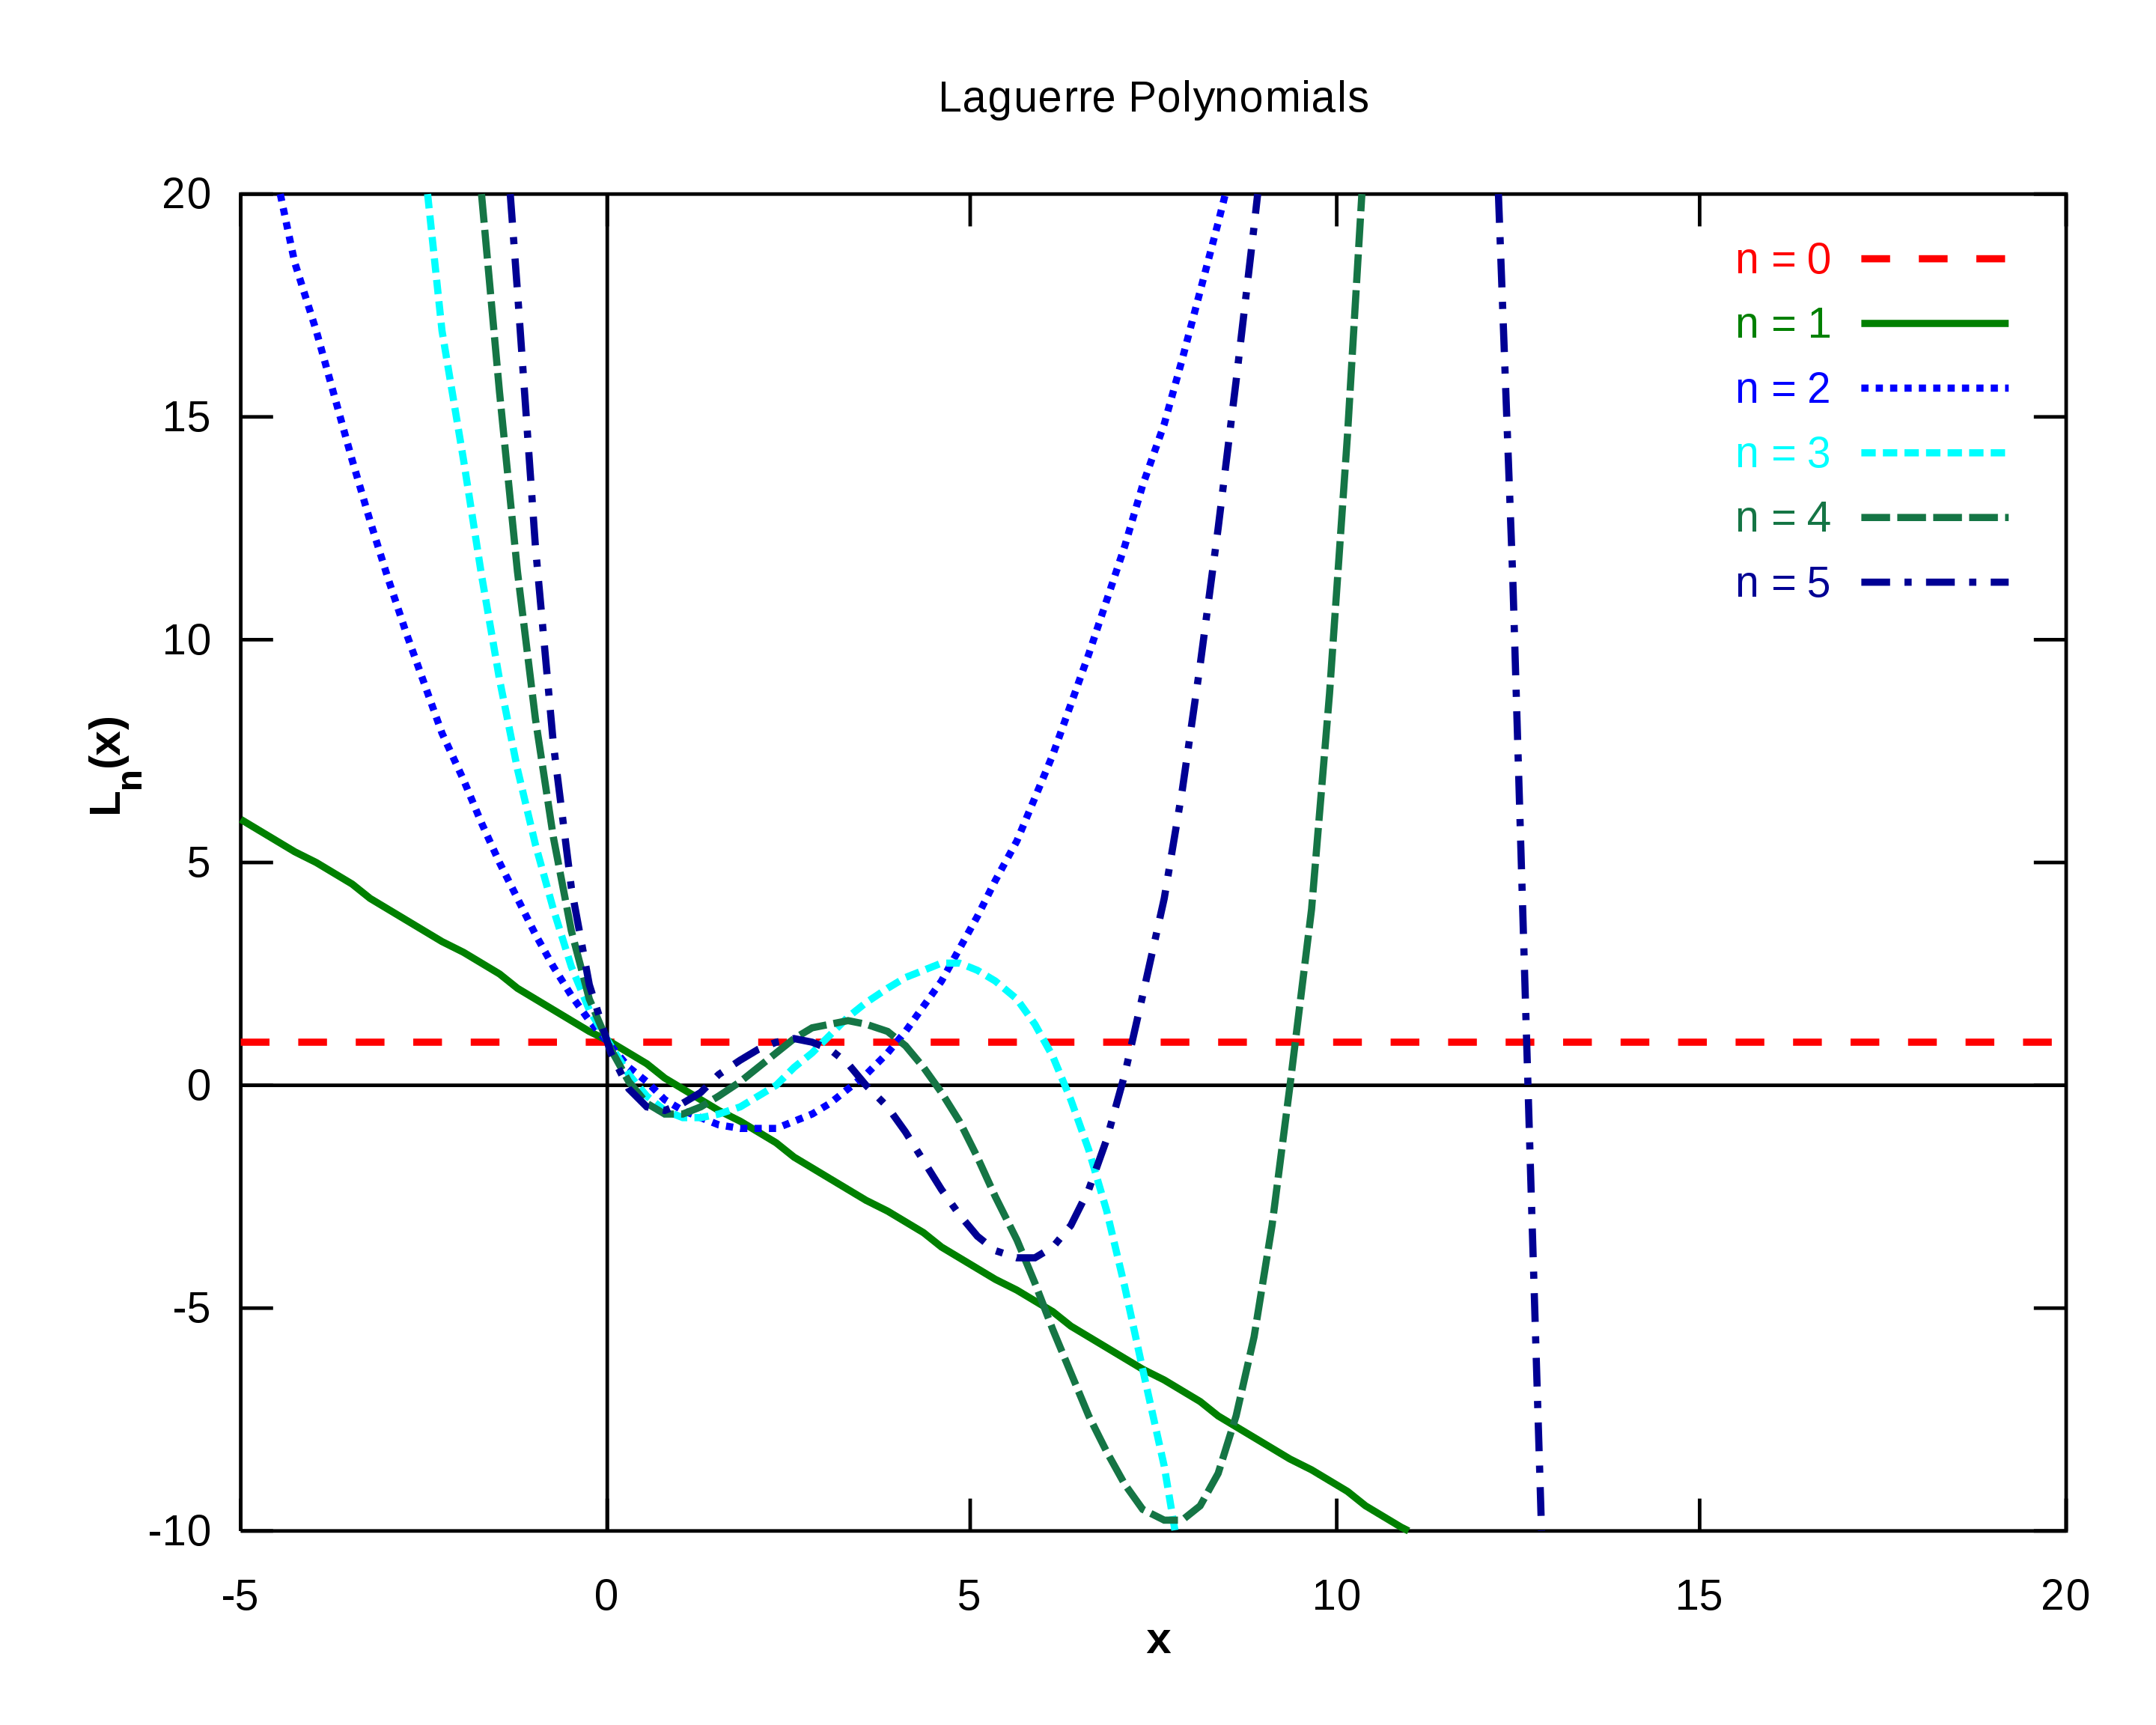
\includegraphics[width=5cm]{Laguerre_poly.png}
\end{center}
\end{itemize}
\end{block}
\end{frame}

\begin{frame}
\begin{block}{Méthode de Gauss-Laguerre}
\begin{itemize}
\item Les $n$ coefficients associés valent respectivement :
\[\myredbox{\forall k =1,\cdots n\quad \omega_k=\frac{1}{(n+1)L'_n(\xi_k)L_{n+1}(\xi_k)}}\]
\end{itemize}

Pour $n=2$ points, on a $\xi_k=2\pm\sqrt{2}$ et $\omega_k=(2\mp\sqrt{2})/4$.

D'où
\[\myredbox{\int_{0}^{\infty}f(x)e^{-x}\de x =\frac{2+\sqrt 2}{4}f( 2-\sqrt 2) + \frac{2-\sqrt 2}{4}f( 2+\sqrt 2) }\]
Maintenant, pour intégrer une fonction $f$ sur $\mathbb{R}^+$, il faut remarquer que

\[\int _{0}^{{+\infty }}f(x)\,{\mathrm  d}x=\int _{0}^{{+\infty }}{\frac  {f(x)}{e^{-x}}}e^{-x}\,{\mathrm  d}x\]
Il reste alors à appliquer la formule de quadrature à la fonction  $g(x)=f(x)e^{x}$
\end{block}
\end{frame}

\begin{frame}
\begin{block}{Méthode de Gauss-Hermite}
\begin{itemize}
\item les points $\xi_k$ sont les racines du polynôme de Hermite $H_n$ :
\[
\myredbox{
\begin{array}{l}
H_{-1}(x)=0 \\
H_0(x)=1\\
H_n(x)=2x\,H_{n-1}(x)-2(n-1) H_{n-2}(x)
\end{array}
}\]
\[H_0(x)=1, H_1(x)=2x, H_2(x)=4x^2-2, H_3(x)=8x^3-12x\cdots\]

\begin{center}
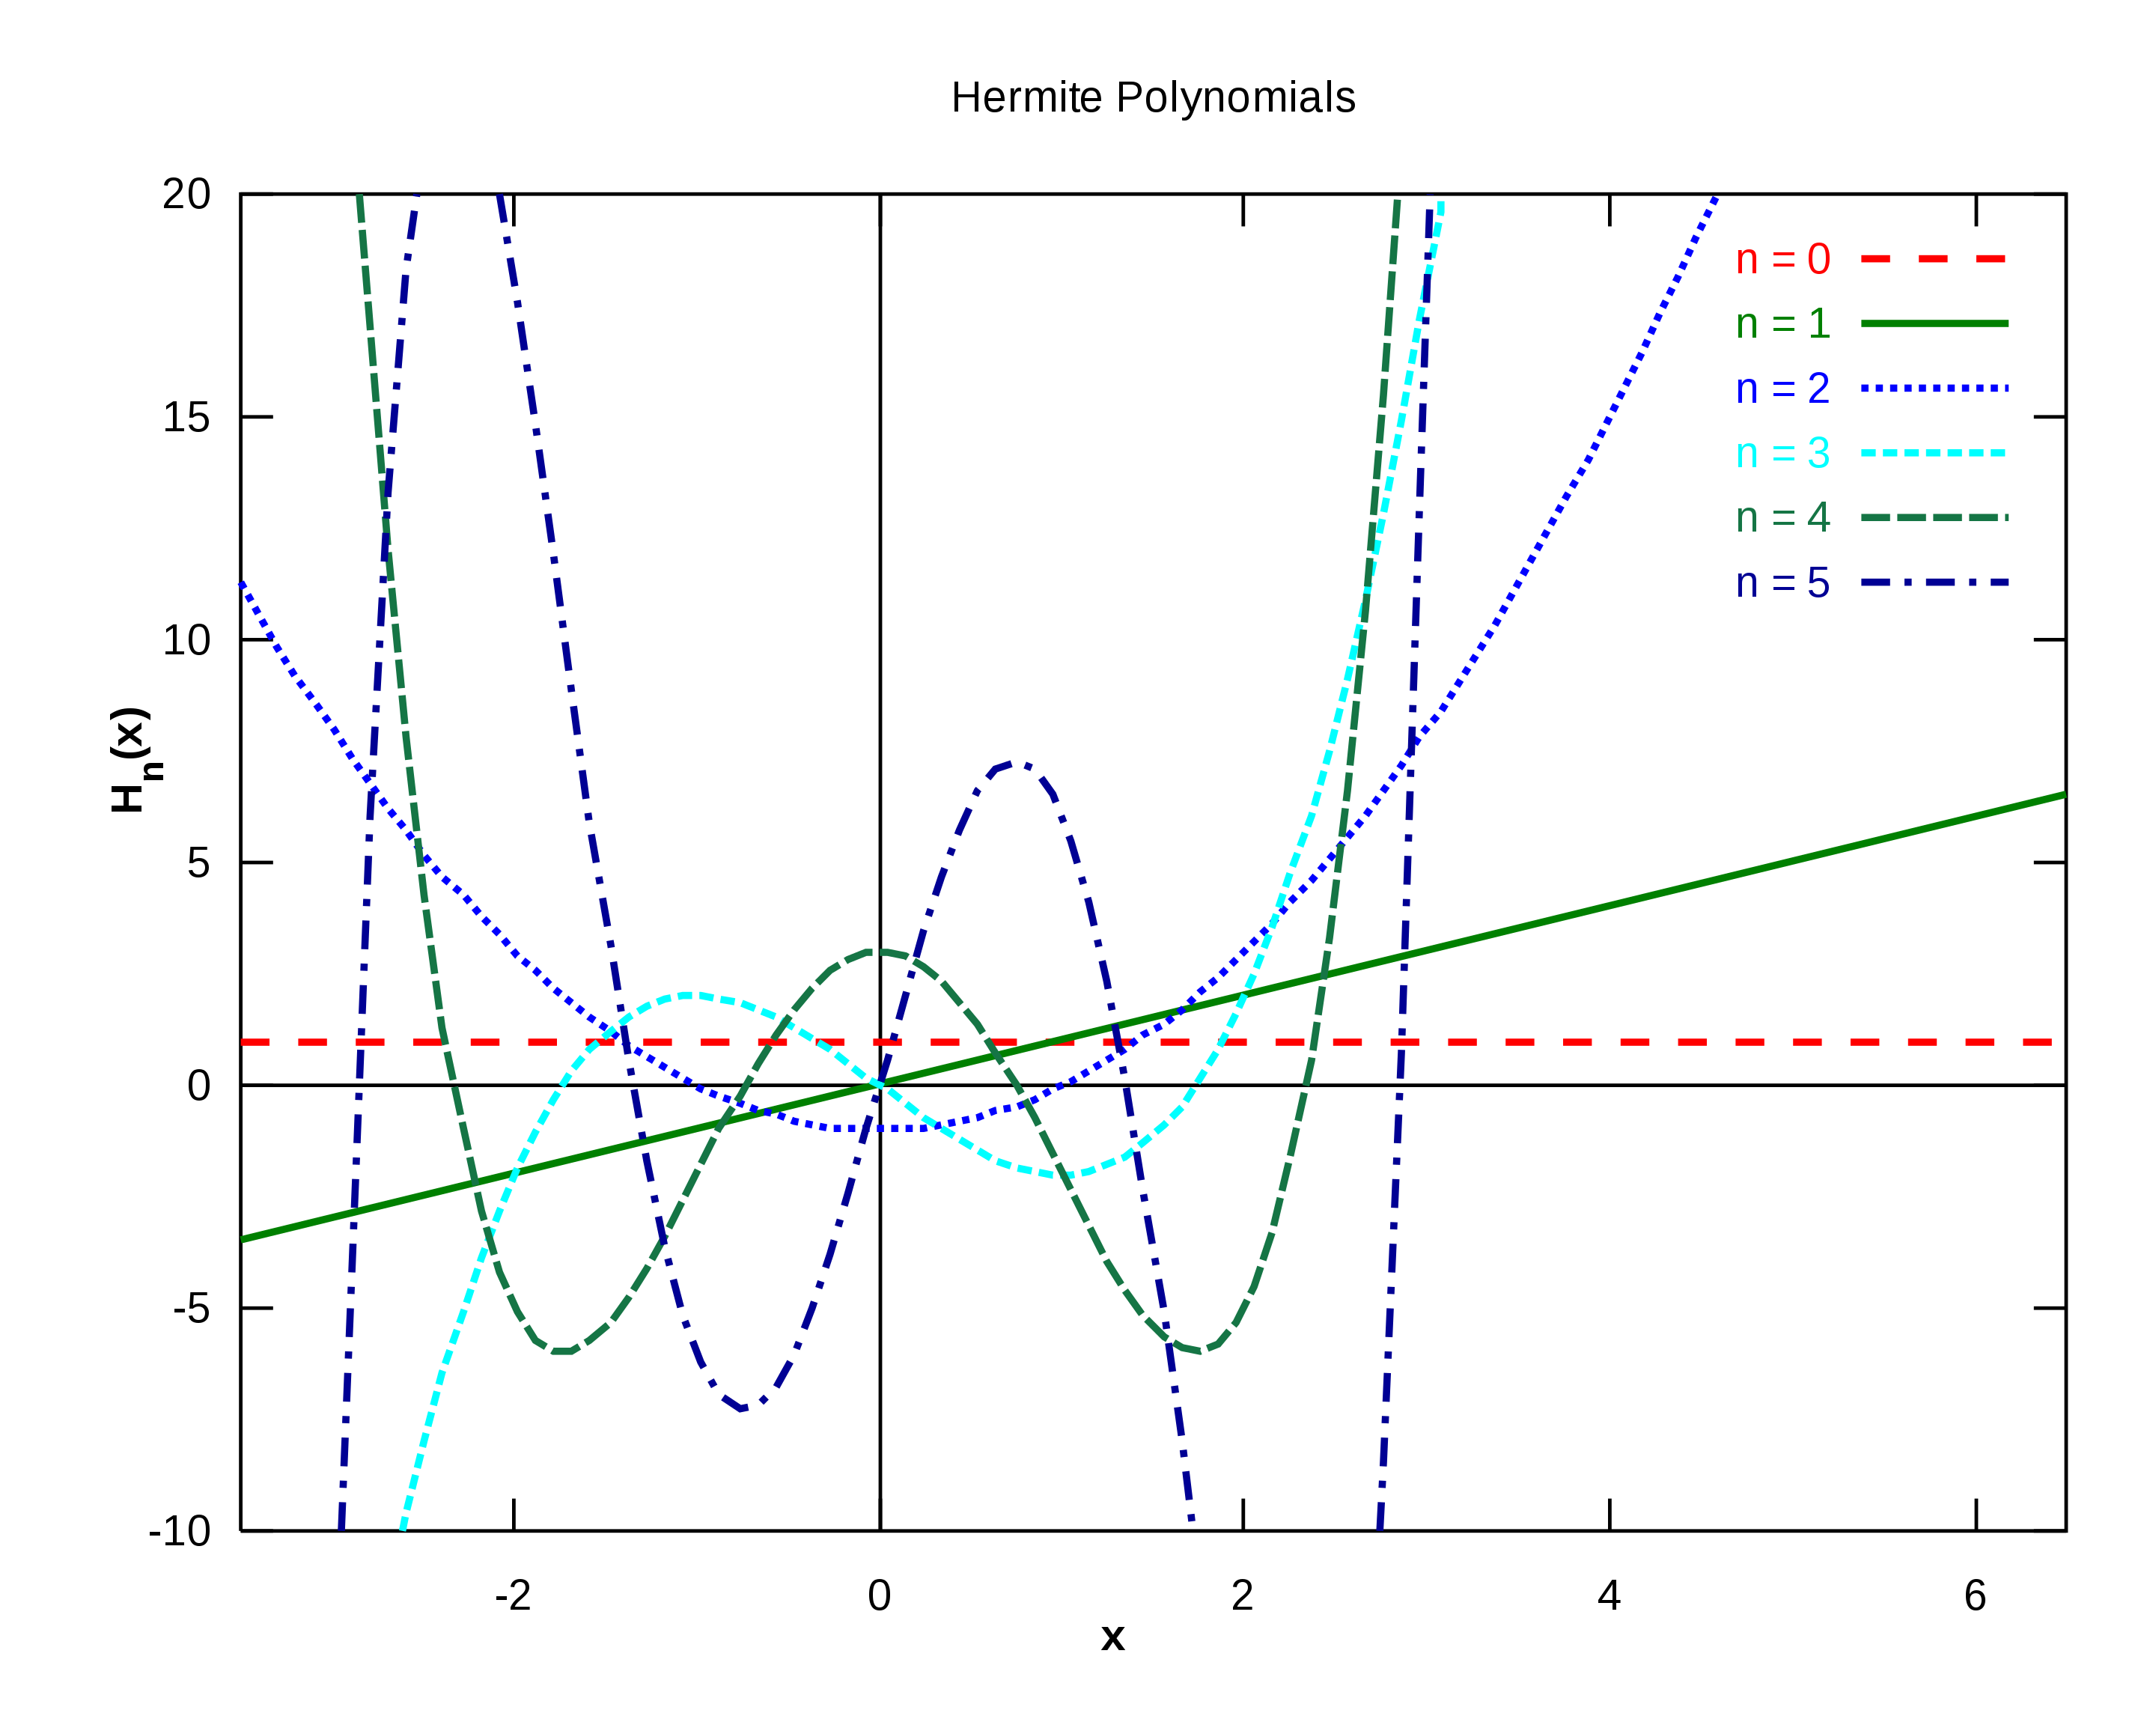
\includegraphics[width=5cm]{Hermite_poly.png}
\end{center}
\end{itemize}
\end{block}
\end{frame}

\begin{frame}
\begin{block}{Méthode de Gauss-Hermite}
\begin{itemize}
\item Les $n$ coefficients associés valent respectivement :
\[\myredbox{\forall k =1,\cdots n\quad \omega_k={\frac  {2^{{n-1}}n!{\sqrt  {\pi }}}{n^2[H_{n-1}(x_{i})]^{2}}} }\]

\end{itemize}

Pour $n=3$ points, on a $\xi_k=-\frac{\sqrt{6}}{2},0,\frac{\sqrt{6}}{2}$ et $\omega_k=\frac{2\sqrt{\pi}}{3(2\xi_k^2-1)^2}$.

D'où
\[\myredbox{\int_{-\infty}^{\infty}f(x)e^{-x^2}\de x =\frac{\sqrt{\pi}}{6}\left(f( -\frac{\sqrt{6}}{2}) +4f(0)+f(\frac{\sqrt{6}}{2})\right) }\]
Maintenant, pour intégrer une fonction $f$ sur $\mathbb{R}$, il suffit d'appliquer la formule de quadrature à la fonction  $g(x)=f(x)e^{x^2}$
\end{block}
\end{frame}

  \end{document}
